\documentclass[12pt]{thapathaliece}

% =========================================
%               Custom Variables
% =========================================
\newcommand\cUniversity{Tribhuvan University}
\newcommand\cDepartment{Institute of Engineering}
\newcommand\cCampus{Thapathali Campus}
\newcommand\cDocumentType{A MAJOR PROJECT PROGRESS REPORT}  % Options: MAJOR/MINOR PROJECT PROGRESS/PROPOSAL REPORT
\newcommand\cTitle{CIRCUITRON: Circuit Recognition, Transformation, and Analysis}
\newcommand\cTitleShort{IEEE report Template and Guidelines}

% =========================================
%          Author Information
% =========================================
% Define only the authors you have (3 or 4)
% Leave \cSubmittedIV and \cSubmittedIVRoll empty for 3 authors

\renewcommand\cSubmittedI{Anveshan Timsina}
\renewcommand\cSubmittedII{Sandesh Dhital}
\renewcommand\cSubmittedIII{Saroj Nagarkoti }
\renewcommand\cSubmittedIV{Utsab Dahal}  % Leave empty for 3 authors, or add 4th author name

\renewcommand\cSubmittedIRoll{(THA078BEI005)}
\renewcommand\cSubmittedIIRoll{(THA078BEI034)}
\renewcommand\cSubmittedIIIRoll{(THA078BEI039)}
\renewcommand\cSubmittedIVRoll{(THA078BEI046)}  % Leave empty for 3 authors, or add 4th roll number

% =========================================
%          Faculty Information
% =========================================

\newcommand\cSupervisor{Er. Kobid Karkee}
\newcommand\cSupervisorTitle{Project Supervisor}
\newcommand\cSupervisorDept{Department of Electronics and Computer Engineering}
\newcommand\cSupervisorAddress{Thapathali Campus, IOE}

%Project Coordinator Info
\newcommand\cProjectCoordinator{Er. Sudip Rana}
\newcommand\cProjectCoordinatorTitle{Project Coordinator}
\newcommand\cProjectCoordinatorDept{Department of Electronics and Computer Engineering}
\newcommand\cProjectCoordinatorAddress{Thapathali Campus, IOE}

%HOD Info
\newcommand\cHOD{Er. Umesh Kanta Ghimire}
\newcommand\cHODTitle{Head of Department}
\newcommand\cHODDept{Department of Electronics and Computer Engineering}
\newcommand\cHODAddress{Thapathali Campus, IOE}

%External Examiner Info
\newcommand\cExternalExaminer{External Examiner}
\newcommand\cExternalExaminerTitle{External Examiner}
\newcommand\cExternalExaminerDept{Deputy General Manager, Civil Aviation Authority of Nepal}
\newcommand\cExternalExaminerAddress{Babar Mahal, Kathmandu}


% Date Formats
\newcommand\cDate{February 2026}
\newcommand\cDateFull{February 15, 2026}


% Optional helper packages used by some guideline chapters
\usepackage{tcolorbox}
\usepackage{tikz}
\usepackage{float}
\usetikzlibrary{positioning,shapes,arrows}

% Glossary entries (define once, print later)
% ABBREVIATIONS/ACRONYMS DEFINITIONS
% Use \gls{key} in text for first use (expands to full form + acronym)
% Subsequent uses show only acronym
% Use \Gls{key} for capitalized version
% Use \glspl{key} for plural
% Use \acrfull{key} to force full form + acronym
% Use \acrshort{key} to force acronym only

\newacronym{ac}{AC}{Alternating Current}
\newacronym{adc}{ADC}{Analog-to-Digital Converter}
\newacronym{ai}{AI}{Artificial Intelligence}
\newacronym{ap}{AP}{Average Precision}
\newacronym{api}{API}{Application Programming Interface}
\newacronym{as}{AS}{Affinity Score}
\newacronym{asgi}{ASGI}{Asynchronous Server Gateway Interface}
\newacronym{bjt}{BJT}{Bipolar Junction Transistor}
\newacronym{cghd}{CGHD}{Circuit Graph Handwritten Diagrams}
\newacronym{cer}{CER}{Character Error Rate}
\newacronym{cli}{CLI}{Command Line Interface}
\newacronym{cnn}{CNN}{Convolutional Neural Network}
\newacronym{cpu}{CPU}{Central Processing Unit}
\newacronym{crnn}{CRNN}{Convolutional Recurrent Neural Network}
\newacronym{crs}{CRS}{Character Region Score}
\newacronym{csv}{CSV}{Comma-Separated Values}
\newacronym{ctc}{CTC}{Connectionist Temporal Classification}
\newacronym{dac}{DAC}{Digital-to-Analog Converter}
\newacronym{dc}{DC}{Direct Current}
\newacronym{dl}{DL}{Deep Learning}
\newacronym{dom}{DOM}{Document Object Model}
\newacronym{eda}{EDA}{Electronic Design Automation}
\newacronym{elan}{ELAN}{Efficient Layer Aggregation Network}
\newacronym{fet}{FET}{Field-Effect Transistor}
\newacronym{fsm}{FSM}{Finite State Machine}
\newacronym{ga}{GA}{Genetic Algorithm}
\newacronym{gnn}{GNN}{Graph Neural Network}
\newacronym{gpu}{GPU}{Graphics Processing Unit}
\newacronym{gui}{GUI}{Graphical User Interface}
\newacronym{hcd}{HCD}{Handwritten Circuit Diagram}
\newacronym{http}{HTTP}{Hypertext Transfer Protocol}
\newacronym{hsv}{HSV}{Hue, Saturation, Value}
\newacronym{ic}{IC}{Integrated Circuit}
\newacronym{ide}{IDE}{Integrated Development Environment}
\newacronym{ieee}{IEEE}{Institute of Electrical and Electronics Engineers}
\newacronym{iou}{IoU}{Intersection over Union}
\newacronym{it}{IT}{Information Technology}
\newacronym{json}{JSON}{JavaScript Object Notation}
\newacronym{llm}{LLM}{Large Language Model}
\newacronym{lmdb}{LMDB}{Lightning Memory-Mapped Database}
\newacronym{lstm}{LSTM}{Long Short-Term Memory}
\newacronym{map}{mAP}{Mean Average Precision}
\newacronym{ml}{ML}{Machine Learning}
\newacronym{nlp}{NLP}{Natural Language Processing}
\newacronym{nms}{NMS}{Non-Maximum Suppression}
\newacronym{ocr}{OCR}{Optical Character Recognition}
\newacronym{pan}{PAN}{Path Aggregation Network}
\newacronym{pcb}{PCB}{Printed Circuit Board}
\newacronym{pht}{PHT}{Probabilistic Hough Transform}
\newacronym{pr}{PR}{Precision-Recall}
\newacronym{rc}{RC}{Resistor-Capacitor}
\newacronym{rcnn}{RCNN}{Region-based Convolutional Neural Network}
\newacronym{rest}{REST}{Representational State Transfer}
\newacronym{rf}{RF}{Radio Frequency}
\newacronym{rl}{RL}{Reinforcement Learning}
\newacronym{rms}{RMS}{Root Mean Square}
\newacronym{sgd}{SGD}{Stochastic Gradient Descent}
\newacronym{spice}{SPICE}{Simulation Program with Integrated Circuit Emphasis}
\newacronym{ui}{UI}{User Interface}
\newacronym{vqa}{VQA}{Visual Question Answering}
\newacronym{yolo}{YOLO}{You Only Look Once}
% \input{src/frontmatter/symbols}

% Initialize glossaries
\makeglossaries



\begin{document}
% =====================
% FRONTMATTER
% =====================

\input{src/frontmatter/_coverBase}
\begin{titlepage}
    \newgeometry{left=1in, right=1in, top=1in, bottom=1in}
    \begin{center}
        \begin{spacing}{1.5}
            
\includegraphics[width=4cm]{src/images/logo.png}

            \vspace{8mm}
            \textbf{\MakeUppercase{\cUniversity}}\\
            \textbf{\MakeUppercase{\cDepartment} }\\
            \textbf{\MakeUppercase{\cCampus}} \\
            \vspace{2em}
            \textbf{\cDocumentType \\ ON \\ }
            \textbf{\MakeUppercase{\cTitle}}\\
            \vspace{2em}
            \textbf{Submitted By:} \\
            \authorTable
            \vfill
            \textbf{Submitted To:} \\
            Department of Electronics and Computer Engineering \\ Thapathali Campus \\ Kathmandu, Nepal \\
            \vfill
            \vspace{1cm}
            {In partial fulfillment for the award of the
                \\
                Bachelors Degree in Electronics, Communication and Information Engineering}
            \vfill
            \textbf{Under the Supervision of} \\
            \cSupervisor \\
            \vfill
            \cDate
        \end{spacing}
    \end{center}
\end{titlepage}


\clearpage
\pagenumbering{roman}

% % Certificate of Approval
\chapter*{CERTIFICATE OF APPROVAL}
\phantomsection
\addcontentsline{toc}{chapter}{CERTIFICATE OF APPROVAL}

\noindent The undersigned certify that they have read and recommended to the
\textbf{Department of Electronics and Computer Engineering, IOE, Thapathali Campus},
a major project work entitled \textbf{``\cTitle''} submitted by
\textbf{\authorList} in partial fulfillment for the award of Bachelor of
Engineering in Electronics, Communication and Information Engineering.
The project was carried out under the special supervision and within the time
prescribed by the syllabus.

\vspace{1em}

We found that the students to be hardworking, skilled and ready to undertake
any related work to their field of study and hence we recommend the award of
partial fulfillment of Bachelor's Degree of Electronics, Communication, and
Information Engineering.

\vspace{2em}

% 2x2 Grid for Signatures
\noindent
\begin{minipage}[t]{0.48\textwidth}
    \rule{6cm}{0.2mm} \\
    \cSupervisorTitle \\
    \cSupervisor \\
    \cSupervisorDept \\
    \cSupervisorAddress
\end{minipage}
\hfill
\begin{minipage}[t]{0.48\textwidth}
    \rule{6cm}{0.2mm} \\
    \cExternalExaminerTitle \\
    \cExternalExaminer \\
    \cExternalExaminerDept \\
    \cExternalExaminerAddress
\end{minipage}

\vspace{3em}

\noindent
\begin{minipage}[t]{0.48\textwidth}
    \rule{6cm}{0.2mm} \\
    \cProjectCoordinatorTitle \\
    \cProjectCoordinator \\
    \cProjectCoordinatorDept \\
    \cProjectCoordinatorAddress
\end{minipage}
\hfill
\begin{minipage}[t]{0.48\textwidth}
    \rule{6cm}{0.2mm} \\
    \cHODTitle \\
    \cHOD \\
    \cHODDept \\
    \cHODAddress
\end{minipage}

\vspace{2em}

\noindent\cDate

% \input{src/frontmatter/declar}
% \input{src/frontmatter/copyright}



% Standard frontmatter
% Copyright Page
\chapter*{ACKNOWLEDGEMENT}
\phantomsection
\addcontentsline{toc}{chapter}{ACKNOWLEDGEMENT}

First, we would like to thank the Department of Electronics and Computer Engineering
for providing us with an opportunity to learn and research on this project. We appreciate
the department’s assistance and recommendations in the selection and hopefully the
successful completion of this project.

Special thanks to our supervisor, \textbf{Er. Kobid Karkee}, for his guidance, invaluable
feedback, and constant support in regards to the project. His expertise and
encouragement have been pivotal in shaping the direction, scope and implementation
of this project. We are also grateful to our project coordinator, \textbf{Er. Sudip Rana}, for his
continuous support and guidance.

Additionally, we would like to thank all of our teachers, friends and other direct and
indirect contributors for their indispensable help, support and encouragement during
our study and execution of the project. We are also grateful to the authors of various
papers that we have referenced for our project.

\vspace{1em}
\noindent \authorTable


\chapter*{ABSTRACT}
\phantomsection
\addcontentsline{toc}{chapter}{ABSTRACT}


\bigskip
CIRCUITRON is an integrated system designed to bridge the gap between traditional 
hand-drawn electrical schematics and modern circuit simulation tools. This project 
consists of a robust pipeline that automates the transformation of handwritten circuit 
diagrams into SPICE-compatible netlists, enabling users to simulate, analyze, and 
interact with circuits in a digitally visualized and editable environment. Leveraging 
deep learning models such as YOLOv7 for component detection, custom OCR for text 
recognition, together with junction-based wire detection, the system has achieved a 
mAP@0.5 of 83\% for component detection, and expects character accuracy of 75\% for 
text recognition, and proper wire and node detection, for horizontal and vertical wires, 
across varied drawing styles. A user-friendly interface allows manual corrections, 
schematic editing, and direct integration with Ngspice for simulation. Additionally, the 
platform incorporates an LLM-powered assistant to answer circuit-related queries, thus 
reinforcing learning through natural language interaction.

\vspace{1em}
\noindent\textit{Keywords: circuit recognition, object detection, SPICE netlist, text recognition, wire detection.}
% Standard document lists

\renewcommand{\contentsname}{TABLE OF CONTENTS}

\renewcommand{\listfigurename}{LIST OF FIGURES}

\renewcommand{\listtablename}{LIST OF TABLES}

\tableofcontents

\clearpage
\listoffigures

\clearpage
\listoftables

% LIST OF ABBREVIATIONS
% Automatically generated from acronyms used in the document
\clearpage
\printglossary[type=\acronymtype,title={LIST OF ABBREVIATIONS}]
\clearpage
% % Print the List of Abbreviations
\chapter*{List of Abbreviations}
\addcontentsline{toc}{chapter}{List of Abbreviations}
\printglossary[type=\acronymtype]


% =====================
% MAINMATTER
% =====================
\clearpage
\pagenumbering{arabic}

\chapter{Introduction}

\noindent ``CIRCUITRON: Circuit Recognition, Transformation, and Analysis'' is a system to convert hand-drawn electrical circuit diagrams into \gls{spice} compatible netlists enabling simulation and graphical analysis along with digital visualization of the circuit in an editable schematic. The system is also to integrate a prompt-based \gls{ai} assistant to help answer queries related to the relevant circuit.

\section{Background Information}

The first step of learning about electrical and electronic circuits involves looking at and hand-drawing said circuits with the necessary components. These hand-drawn circuit diagrams continue to play an important role in electronics education and early-stage hardware design due to their ease of use, speed, and accessibility. However, such hand-drawn diagrams prove to be limited in their utility in the current education landscape that prioritizes intuitive and visual understanding as they require significant mental gymnastics to facilitate any form of analysis of the circuits, especially when the change in parameters is incorporated.

A slew of rather easy-to-use circuit simulation and analysis tools such as \gls{ltspice} and KiCad exist, of course; and they continue to foster visual learning and analysis of circuits of a range of complexities. But these traditional \gls{eda} tools lack the capability to accept hand-sketched circuit diagrams as input. Instead, users are required to redraw the circuits in software using \gls{gui} tools or by manually entering \gls{spice} netlists; steps that are both tedious and error-prone \cite{reddy2021handdrawn, sertdemir2022img2sim}. Be it due to the (admittedly not very steep yet inconvenient) learning curve of these tools or just the additional effort of having to redraw a circuit digitally (the dullness of which only goes up with circuit complexity), the instructors as well as the students often tend to neglect arguably essential simulation-based intuitive teaching and learning. This again encourages the same long-established rote learning practice instead of ushering in a new and perceptively intuitive way of understanding circuits and electronics at large. And it has been long proven that students tend to perform better when given the appropriate simulative manipulation and concept clarification tools, especially in the context of electrical and electronics circuits \cite{chen2011efficacy}. It then follows that the reluctance to use such tools is actively hindering the students' potential. Thus, the use of visual manipulative simulation tools is the need of the hour. In fact, it has been the need of the hour for quite a while. But, due to a lack of any uber-convenient method, it is yet to be popularly embraced, primarily in technologically nascent countries such as Nepal.

\section{Motivation}

In recent years, the mantra of the modern world has seemingly become ``adapt or die''. The society regularly stomps on the tech-illiterate to make way for the ones willing to champion the use of new and shiny tools in all aspects of their lives. In an increasingly globalized economy, this is especially true for the up-and-coming students who need to compete with other students all over the world relying solely on their understanding of subject matter in their particular fields. In such case, it becomes essential that they are given the tools to enhance their learning and understanding even by minor increments. In the context of electronics, circuits are the fundamental building blocks that permeate each and every aspect of our ``teched-out'' world and it is important for learners in the field to have an intuitively in-depth understanding of this fundamental ingredient. Thus, there exists a motivation for a hassle-free method to analyze and understand circuits to deepen the necessary conception and comprehension.

The motivation stems not only from a deep-seated commitment to give the instructors and students tools to easily visualize and analyze circuits in the belief that it will genuinely improve the quality of professionals and engineers born out of universities, but also from the personal experience of the members involved in this project. As the electronics engineers of the near future who have had and will continue to have to deal with circuits in one form or another, the members involved in this project are uniquely positioned to understand the plight of a beginner in the study of electronics. And a tool which can convert a hand-drawn circuit into a digital schematic and also allow for analysis would go a long way in alleviating that plight.

\section{Problem Statement}

The \gls{eda} tools currently available do not support the direct transformation of hand-drawn circuit images into simulation-ready schematics. There exist a few nascent prototypes for the same but there seems to be no widely adopted, robust, and user-friendly pipeline that combines component recognition, reliable wire connectivity, schematic generation and simulation, whether by itself or by integration with \gls{spice} simulators. 

``CIRCUITRON: Circuit Recognition, Transformation, and Analysis'' project aims to create an integrated system capable of first, recognizing and digitizing hand-drawn circuits into editable schematics and then allowing the user to analyze those circuits through graphs using \gls{spice}-compatible netlists with an added \gls{ai} assistant to handle related queries.

\section{Project Objectives}

\begin{itemize}
    \item To automatically convert hand-drawn circuit diagrams into \gls{spice}-compatible netlists for simulation.
    \item To visualize the circuit in an editable schematic in addition to an \gls{ai} assistant for handling simple, relevant queries.
\end{itemize}

\section{Project Scope and Applications}

\subsection{Project Scope}

This project focuses on the development of a software pipeline that accepts scanned or photographed images of hand-drawn electrical circuits and transforms them into \gls{spice}-compatible netlists for simulation as well as editable schematics through an intermediate integrated data structure to facilitate the transformation. The scope includes detecting common circuit components and their values in mentioned units, inferring wire connectivity with junction recognition and generating a circuit diagram with simulation capabilities. Additionally, the system is to incorporate an \gls{llm}-based query-solving \gls{ai} assistant. The system will support basic circuits and components but will exclude any form of advanced circuit transformation and analysis such as in circuits associated with \gls{rf}, mixed-signal, or \gls{pcb} designs.

\subsection{Project Applications}

\begin{itemize}
    \item \textbf{Educational utility:} The system is foremost, to be an educational tool designed to assist students and instructors in conveniently digitizing circuit diagrams and understanding circuit behavior through limited simulation and interactive Q\&A.
    \item \textbf{Lightweight prototyping:} The project is to enable rapid comparison of hand-drawn designs with \gls{spice} simulation results early in the design process for quick feedback and validation.
    \item \textbf{Mobile simulation tool:} The project in its final form can facilitate quick on-the-go analysis of circuits for students and potentially, field engineers as well.
\end{itemize}

\subsection{Project Limitations}

Despite its innovative concept, the system is constrained by several factors. First, its accuracy depends heavily on the quality and clarity of input images; low-resolution or messy sketches may lead to recognition errors. The fix for this would obviously be more rigorous training on appropriate training data to chip away at the error but finding the ideal dataset with enough examples for all kinds of components and circuits has proven challenging. Additionally, the system is to support only a fixed set of commonly used components and may fail on rare or user-defined symbols. Wire connectivity assumes standard drawing practices however there is no one way to draw a circuit diagram; non-standard or overlapping wires as well as complicated circuits may confuse the parser. Moreover, the system is to lack a simulation engine of its own and instead use an open-source tool like Ngspice, which not only affects the seamlessness of the user experience but also limits the simulation capabilities to that of Ngspice. For instance, Ngspice needs \gls{spice} models to be imported for complicated circuit elements such as \gls{adc}, \gls{dac}, timers, etc. This means even if the system can recognize these hand-drawn circuit elements, it will not be able to simulate their functionality.
\chapter{LITERATURE REVIEW}

Hand-drawn circuit recognition and digitization, while not a vastly researched area, has a few notable examples of its implementation. Most of the study and implementation related to this has been done on classifying the different circuit components (like battery, resistors, inductors, etc.) and there's not much on arguably the more difficult aspect of circuit recognition: node and wire connectivity. For instance, in a 2021 study, 20 different components were classified from self-made hand-drawn circuits with the recognition accuracy of 97.33\% \cite{adnan2021cnnbased}.


In one of the oldest studies on the automatic recognition of hand-drawn circuits, an approach of identifying the components first and then the node segments (taking into consideration their spatial relationship) was implemented, achieving an accuracy of 86\% for components and 92.5\% for the nodes. The node segments were then traced assuming wire between them, considering a variety of hard-coded conditions \cite{edwards2000machine}. In a recent 2024 research, a couple of \gls{uk} engineers were successful in digitizing images of electrical circuit schematics using a novel pattern-recognition methodology and custom-trained \gls{ocr} model achieving respective success rates of 86.4\% and 99.6\% \cite{kelly2024digitizing}. This, however, was trained on printed/computer-made circuit diagrams, not hand-drawn ones and also isn't able to understand the values of the circuit components.



To overcome the limitations of \glspl{cnn} in understanding circuit topology, graph-based methods have gained traction. Circuit2Graph, a pipeline that transforms circuit diagrams into graph structures where nodes represent components and edges denote electrical connections was introduced in 2023. Using \glspl{gnn}, their system achieved 97.9\% accuracy on circuit classification tasks, outperforming traditional methods \cite{yamakaji2023circuit2graph}. This approach demonstrated that \glspl{gnn} can effectively model the global structure of a circuit, even when visual features alone are insufficient. Similarly, Bayer et al.\ \cite{bayer2023instance} used Mask \gls{rcnn} for instance segmentation of components in hand-drawn diagrams, followed by graph extraction techniques to infer connections. Their model achieved around 94\% mask accuracy, but they noted that symbol recognition was ``reasonable, yet incomplete,'' especially in more complex drawings or where handwriting was less consistent. A paper published in the International Research Journal of Engineering and Technology proposed a two-step method for electronic circuit diagram detection and recognition; first detecting and classifying the components present in the circuit and then labeling the classified components to form a string which is then fed to an \gls{fsm} system for circuit recognition \cite{abhinav2020electric}.



With the use of YOLOv5 for detection of circuit components and Probabilistic Hough transform-based solution for node recognition and taking in hand-drawn circuits, a couple of Indian engineers were successful in achieving not only a \gls{map} of 98.2\% in component detection but also a near-real time generation of circuit schematic with an accuracy of 80\% \cite{reddy2021handdrawn}. However, their circuits were not labelled which is to say the values for the battery (in volts), resistance (in Ohms), etc.\ were not written in the circuit. Another very recent study suggested a three-step process to detect and identify the circuit and its components with the steps including detection of components, detection of lines and their junctions and then the detection of text placed near the components and then combining the data from these three streams into a \gls{json} format to eventually derive a netlist from \cite{hemker2024schematics}. This is a similar workflow to the one this project intends to use; however, the scope of our project is much larger owing to the fact that an editable schematic is to be delivered on top of taking in hand-written circuit diagrams as opposed to generating a netlist from a digital schematic.

Netlist generation is also a very critical aspect of this domain. While traditional \gls{eda} tools such as KiCad and \gls{ltspice} support netlist export from manually created schematics, they do not allow direct image-to-netlist conversion \cite{kicad2024spice}. This limitation was addressed with Img2Sim; an artificial neural network-based system that detects components, infers connectivity, and outputs a complete \gls{spice} netlist. Their model reported over 90\% accuracy in topology extraction and represents one of the first functional pipelines to translate a hand-drawn circuit into a ready-to-simulate format \cite{sertdemir2022img2sim}. However, Img2Sim and similar systems typically require clean input images and are limited to a predefined set of components, reducing their robustness in real-world use cases. While the feasibility of such pipelines is now evident, a generalized, accurate, and open-source solution that goes the extra mile to also visualize the circuits digitally remains unavailable.



Parallel to recognition and netlist generation, visual question answering (\gls{vqa}) for circuits is emerging as a useful educational application. CircuitVQA is a dataset containing more than 115,000 question-image pairs based on 5,725 unique circuits. It covers approximately 70 symbol types and supports the training of transformer-based \gls{vqa} models capable of answering questions like ``What is the function of R1?'' or ``Is this a voltage divider?'' Early experiments demonstrated that models fine-tuned on CircuitVQA outperformed generic \gls{vqa} systems, indicating the importance of domain-specific training. Meanwhile, large language models (\glspl{llm}) such as GPT-4 have also been explored for circuit explanation tasks. For instance, the SPICEPilot framework attempts to generate and interpret \gls{spice} code using GPT-based models \cite{vungarala2024spicepilot}. However, these general-purpose models often fail to respect domain conventions, such as valid W/L ratios or simulation types, resulting in inaccurate outputs.



Finally, simulation integration plays a vital role in validating and interacting with generated circuits. Ngspice, an open-source simulation engine, is widely used in research and is natively supported in KiCad. It enables \gls{dc}, \gls{ac}, and transient analysis, making it suitable for most educational and prototyping needs. In contrast, commercial tools like Simulink and PSpice provide broader capabilities but are cost-prohibitive. Some research efforts, including Img2Sim, have leveraged open standards to generate \gls{spice} files compatible with tools like Ngspice or PSpice. Other projects utilize Python-based libraries such as PySpice to enable automated simulation directly within a code-driven environment which is exactly how this project intends to accomplish its simulation needs.



While significant progress has been made in component recognition and value comprehension, connectivity inference, netlist generation, and interactive Q\&A, existing systems remain fragmented or limited in scope. An end-to-end system that combines all these elements into a user-friendly platform remains a critical need for both educational and practical applications.
\chapter{REQUIREMENTS ANALYSIS}

\section{Software Requirements}

\subsection{Python Libraries}

\gls{python} Programming Language is the heart of the machine learning aspects of the project as well as parts of the backend. \gls{python} with its suite of various packages and libraries is used to facilitate the implementation of models for object detection, text recognition, and even simulation visualization.

\begin{itemize}
    \item \textbf{NgSpice and PySpice:} After detecting and extracting relevant circuit elements, the project aims to simulate the circuit. \gls{ngspice} is the open-source \gls{spice} simulator for electric and electronic circuits which takes in netlists and enables the simulation and analysis of circuits. And, \gls{pyspice} is a \gls{python} library that provides bindings to \gls{ngspice} to build and simulate circuits entirely within \gls{python}.
    
    \item \textbf{PyTorch and TensorFlow:} PyTorch and TensorFlow, both \gls{dl} libraries, which serve as the backbone for training and deploying machine learning models used in the project pipeline. They are used to first integrate existing models, specifically YOLOv7 and \gls{ocr}, into the project and then also fine-tune and train them depending on the need. Also, the seamless integration of these libraries with other widely used \gls{python} libraries, including NumPy and Pandas, streamlines data preprocessing and manipulation. Both PyTorch and TensorFlow, while having different strengths, serve similar purposes for this project and use of one over the other just comes down to personal preference and convenience.
    
    \item \textbf{Numpy:} Numpy is an open-source \gls{python} library for all tasks related to numerical computing and data manipulation. CIRCUITRON uses Numpy for array manipulation and pixel-level operations on images. Numpy seamlessly integrates with OpenCV and helps streamline the fundamental processes of image processing like converting images into matrices, performing image-wide as well as element-wise operations important for augmentation, thresholding and segmentation.
    
    \item \textbf{OpenCV:} OpenCV is the primary library for pre-processing the circuit images and performing low-level computer vision tasks. It is used in almost all aspects of image processing in the project like thresholding, edge detection, geometric augmentations, contour detection, morphological operations (dilations, erosion) as needed. These operations help in extracting meaningful visual information before feeding the data into the models.
    
    \item \textbf{Pandas:} Pandas provides data structures, such as data frames, that allow for efficient handling and manipulation of structured data. It offers functions for reading and writing data from various file formats, data cleaning and preprocessing, filtering and selecting data, grouping and aggregating data, and more. Pandas is used in the project to organize structured data related to the circuit components and their properties which includes storing component lists with attributes like label, value, position, and orientation, managing the intermediate data between detection, parsing, and netlist generation, and exporting tables or logs for debugging or evaluation.
    
    \item \textbf{Matplotlib and Plotly:} Matplotlib is a widely used data visualization library in \gls{python}. Matplotlib is used in the project for visualizing the performance metric scores in graphs. Furthermore, it is to be used for plotting simulation outputs with integration with \gls{pyspice}. Plotly is another library for data visualization which supports interactive diagrams (handy for showing simulation graphs in motion).
    
    \item \textbf{Scikit-learn:} In context of the project, Scikit-learn is used for post-processing tasks such as clustering junction points, filtering outliers, or classifying ambiguous component types after initial detection. It includes tools for data splitting, metrics, and evaluation which are extremely useful during model development and benchmarking. Additionally, it can assist in component matching, value prediction, or validation models if required.
    
    \item \textbf{Seaborn:} Seaborn is a \gls{python} data visualization library based on Matplotlib, designed for creating statistical graphics with attractive default styles. It is used to visualize distributions, such as accuracy of component detection, or \gls{ocr} confidence scores. It is essentially a wrapper for Matplotlib which makes working with graphs more convenient. It can also be used with Pandas to plot trends in simulation outcomes (say, voltage over time across components).
    
    \item \textbf{Hugging Face:} Hugging Face provides a large hub of pretrained transformer models for \gls{nlp}, vision, and more, along with the transformers \gls{python} library. It will be used in the project to integrate \glspl{llm} for answering circuit-related queries.
    
    \item \textbf{LangChain:} LangChain is a framework that helps build applications powered by \glspl{llm}, focusing on prompt engineering, chaining logic, memory, and tool use. It will be used to build the \gls{llm}-based \gls{ai} assistant for the user interface by integrating circuit data (netlist, components, simulation results, schematics) to provide context-aware answers.
    
    \item \textbf{LangGraph:} LangGraph extends LangChain to allow for multi-agent or multi-step workflows using graph-like state machines. It can be used to build structured conversational workflows where the \gls{ai} assistant interacts with different parts of the circuit data pipeline while maintaining session history.
\end{itemize}

\subsection{YOLOv7}

The YOLOv7 model is used to detect and classify circuit components in hand-drawn circuit images. It outputs bounding boxes, class labels, and confidence scores for each detected component. YOLOv7 is selected due to its superior detection accuracy, efficient training capabilities, and support for multiple object scales through its enhanced architecture. Compared to previous versions like YOLOv5, YOLOv7 delivers better performance in terms of \gls{map} and inference speed.

\subsection{DTRB Framework-Based OCR}

A \gls{crnn}-based \gls{ocr} model trained from scratch, following the DTRB design philosophy for recognizing text is vital for the project as it is the core technology which reads and understands the component values and units of circuit elements. This was chosen for the project because, foremost, other ready-made \gls{ocr} models failed to perform well even after some fine-tuning.

\subsection{KiCad Symbol Library}

KiCad is a free, open-source \gls{eda} suite which offers its libraries to be used freely to build any educational project. The project intends to use the KiCad symbols library, specifically, in order to simply extract the component symbols standardized by KiCad rather than building the icons/representations for components from scratch for use in the frontend schematic.

\subsection{Coding and Training Platforms}

\begin{itemize}
    \item \textbf{Google Colab:} Google Colab is a cloud-based platform that offers a Jupyter notebook environment for developing deep learning systems. For this project, Google Colab provided with \glspl{gpu} for free, which significantly accelerated the training process, enabling experimentation with larger models and datasets. Colab also comes pre-installed with popular deep learning frameworks such as TensorFlow and PyTorch, widely used for \gls{ml}-related tasks. Leveraging these frameworks, YOLO (v5 and v7) and \gls{ocr} were implemented and experimented on.
    
    \item \textbf{Kaggle:} Kaggle is a multi-faceted online platform popular for data science competitions, datasets, code sharing and model training. It was primarily used to find relevant datasets (\gls{cghd}, \gls{vqa}, \gls{hcd}), code sharing and model training. The dataset of choice for this project was also found in Kaggle. Additionally, it provided a fully hosted environment with popular \gls{python} libraries such as Pandas, Numpy, Tensorflow, PyTorch pre-installed to make implementing and training models convenient, especially with its integration with Google Colab. Its free cloud computing service providing 30 hours of \gls{gpu} use per week proved indispensable in accelerating the training and testing of different models.
    
    \item \textbf{Lightning AI:} Lightning AI is a cloud workspace, similar to Google Colab and Kaggle, which specializes in helping build agents and train models without any tedious setup. Most importantly, through the use of a student account, it allows for the use of extremely powerful \glspl{gpu} for free (for a reasonable amount of time). Among all the cloud computing services used for the project, Lightning AI proved the most invaluable for implementing and training the models as the \glspl{gpu} it allotted were super-fast and saved a ton of time during the tedious and time-consuming process.
    
    \item \textbf{Visual Studio Code:} The local \gls{ide} of choice for this project is VS Code due to its extensive features auto completion, syntax highlighting, and copilot integration. Additional features are further integrated by the use of a suite of easy-to-use extensions which are tailored for each individual project member in their setup as needed. All the code to be run locally is run on VS Code and further down the line, its utility is expected to increase ten-fold during the web development phase.
\end{itemize}

\subsection{Web Development}

Although the web development part of this project has not kicked into gear as of yet; following are the tools and technologies expected to be used in the process:

\begin{itemize}
    \item \textbf{Reactjs:} Reactjs will serve as an integral technology underlying the dynamic front-end interfaces to be developed for the project. The frontend for this project is expected to include dynamic elements like dragging, erasing, resizing, etc. of the circuits and circuit elements, and Reactjs is expected to fulfill these requirements with convenience and speed through the use of its features like virtual \gls{dom} abstraction, distinction of code into reusable logic and presentation buckets, etc. as well as compatible packages like react-draggable.
    
    \item \textbf{Next.js:} Next.js is a React-based web framework that enables the development of fast, scalable, and server-rendered web applications. It provides features such as routing, server-side rendering, and \gls{api} integration, which are essential for building a responsive and user-friendly frontend. In this project, Next.js is used to develop the client-side interface, enabling efficient interaction with the backend services and smooth visualization of recognition results.
    
    \item \textbf{Chart.js:} Chart.js is a lightweight JavaScript library used for creating interactive and visually appealing charts and graphs in web applications. Chart.js is used to visualize analytical results such as performance metrics, recognition accuracy, confidence scores, and statistical summaries on top of the graphs generated after simulation in a clear and intuitive manner. Its ease of integration with modern frontend frameworks and support for real-time data updates make it suitable for presenting system outputs effectively.
    
    \item \textbf{FastAPI:} FastAPI is a modern, high-performance \gls{python} web framework used for building RESTful \glspl{api}. It is designed for rapid development, high execution speed, and automatic generation of interactive \gls{api} documentation. In this project, FastAPI is used to implement the backend services that handle requests from the frontend, manage data exchange, and interface with the text recognition and analysis modules. Its native support for asynchronous operations and integration with Pydantic ensures efficient request handling and robust data validation.
    
    \item \textbf{Uvicorn:} Uvicorn is a high-performance \gls{asgi} server used to run asynchronous \gls{python} web applications. It is commonly used to serve FastAPI-based backend services due to its low latency and efficient handling of concurrent requests. In this project, Uvicorn is responsible for hosting the backend \gls{api}, ensuring fast communication between the frontend application and the \gls{ocr} processing modules.
    
    \item \textbf{Pydantic:} Pydantic is a \gls{python} library used for data validation and schema definition using type annotations. It ensures that data exchanged between the frontend and backend conforms to predefined structures and types. In this project, Pydantic is used to define request and response models, improving data integrity, and reducing runtime errors.
    
    \item \textbf{MongoDB:} MongoDB is a NoSQL database which stores data in \gls{json} documents organized into collections. It is to serve the database needs for this project which enables functionalities like saving a digital schematic with its component values, simulation result storage, etc.
    
    \item \textbf{Github:} Github is a platform to store, manage and share code with integrated version control. Github enabled effective sharing and backing up of all the code involved in this project as of yet and allowed for all the participants to be on the same page at any given time. Github is expected to be used extensively throughout the project.
\end{itemize}

\section{Feasibility Study}

\subsection{Technical Feasibility}

Technical Feasibility assesses whether the project can be developed using available resources and expertise. The system leverages well-established technologies such as \gls{python}, OpenCV, custom \gls{ocr}, YOLOv7, Ngspice, FastAPI, Next.js, all of which are stable and widely supported. For component detection, YOLOv7 provides effective object recognition, making it suitable for identifying handwritten circuit symbols. Wire and node detection rely on proven techniques like skeletonization, junction-based wire detection, and clustering (e.g., K-means). Optical Character Recognition (\gls{ocr}) is handled effectively using custom-trained \gls{ocr}, ensuring accuracy even with noisy text. Simulation is facilitated through Ngspice \gls{cli} in tandem with Pyspice. The team consists of skilled electronics and software engineers proficient in these technologies. The primary technical risk involves processing low-quality or cluttered circuit images, but the system is to include manual correction features to mitigate this. Overall, the project is technically feasible, with all necessary tools available and a well-matched skill set.

\subsection{Economic Feasibility}

Economic Feasibility examines whether the project is cost-effective and offers a good return on investment. The estimated costs include NPR 20,000 for computation (Google Colab Pro and cloud \glspl{gpu}), NPR 4,000 for hosting and storage (domain, cloud storage, and database), NPR 2,160 for \gls{ieee} membership (access to research journals), and NPR 15,000 for miscellaneous expenses (printing, presentations, memberships, etc.). Data collection and software licenses incur no cost since open-source datasets and tools are utilized. The total estimated budget is approximately NPR 41,160. Given its potential as an educational tool, the project could even be commercialized for academic institutions. The project is considered economically feasible due to its low development cost for the value it has to the education field.

\subsection{Operational Feasibility}

Operational Feasibility evaluates whether the system will function effectively in real-world scenarios. The tool addresses a genuine need by simplifying the conversion of hand-drawn circuits into simulations, eliminating manual redrawing. Its user-friendly interface allows optional manual edits to improve reliability, and cross-platform accessibility is ensured through a web-based (Next.js and FastAPI). Minimal training is required due to its intuitive design, and performance is optimized with near real-time processing using YOLOv7 and efficient \gls{ocr} techniques. The modular architecture ensures easy maintenance, and the system can be scaled to support additional features in the future. The project is considered operationally feasible.

\subsection{Time Feasibility}

% The project is to be developed in two sequential phases, with Phase A focusing on implementing the core functionality including the circuit recognition and text extraction engine, and netlist generation within a basic web framework. Upon successful completion and testing of these foundational elements, Phase B will expand the system by developing the full web application, integrating NgSpice for simulations with a user-friendly \gls{ui} to display and edit schematic diagrams, and implementing the \gls{ai} question-answering feature; all while maintaining consistency with the pre-designed wireframes. A two-week buffer period has been planned between phases to accommodate thorough testing and necessary adjustments, with Phase B work commencing only after Phase A components have been fully validated. This structured approach ensures the maintenance of design integrity while progressively enabling the deliverance of more advanced features. As of yet, Phase A is advancing at a reasonable pace. The project is considered feasible from a time perspective.
The project has to be developed in two sequential phases, with Phase A focusing on implementing the core functionality including the circuit recognition and text extraction engine, and netlist generation within a basic web framework. This phase has been successfully completed and tested.

Phase B is supposed to expand the system the system by developing the full web application, integrating NgSpice for simulations with a user-friendly UI to display and edit schematic diagrams, and implementing the AI question-answering feature; all while maintaining consistency with the pre-designed wireframes. A two-week buffer period had been planned between phases to accommodate thorough testing and necessary adjustments, with Phase B work commencing only after Phase A components have been fully validated. This structured approach ensures the maintenance of design integrity while progressively enabling the deliverance of more advanced features. As of yet, phase A has been completed and phase B is also nearly done, and advancing at a reasonable pace. The project is considered feasible from a time perspective.

\chapter{SYSTEM ARCHITECTURE AND METHODOLOGY}

\section{Block Diagram}

The process of converting a handwritten circuit diagram into a structured netlist involves a series of coordinated steps, each step feeding into the next, designed to detect, extract, and represent pictorial information in a machine-readable format and then using this data for simulation and schematic generation.

\begin{figure}[H]
    \centering
    
\includegraphics[width=\textwidth]{src/images/figures/block_diagram.png}
    \caption{Block Diagram of the CIRCUITRON System}
    \label{fig:block-diagram-circuitron}
\end{figure}

The high-level architecture of the CIRCUITRON system is visualized in the block diagram in Figure~\ref{fig:block-diagram-circuitron}. Each step involved in the hand-drawn image to simulation-ready schematic pipeline is elaborated as follows.

\subsection{Preprocessing}

At first, the circuit information (components, component values, units, wire intersection, etc.) needs to be extracted out from the hand-drawn image. Appropriately fine-tuned ML and DL models are to be used for each of these steps which will be elaborated on in later subsections, however, for any sort of detection to happen, the image needs to first be pre-processed. Preprocessing for this not only includes image manipulation tasks but also conversion of the dataset annotations into appropriate formats to maintain compatibility with the component detection and text recognition models. The dataset of choice is in the Pascal VOC format which is incompatible with the models that are intended to be used in the pipeline and hence need to be converted. The code for this conversion with examples will be discussed in the implementation section.

Furthermore, image preprocessing, which includes steps like denoising, contrast and brightness enhancement (for improved clarity) is a vital step in readying the dataset for training any and all models. However, geometric augmentations, especially rotation, is not appropriate for this project.

Among the various available preprocessing techniques, the ones to use are to be selected with careful consideration of the type of images available in the dataset as well as the models in use. Besides image manipulation using various techniques, preprocessing also includes splitting the dataset into training, validation and testing subsets as appropriate.

\subsection{Circuit Component Detection}

A critical step in the pipeline is the accurate detection of circuit components from hand-drawn schematic images. This task is addressed using a real-time object detection algorithm capable of identifying and localizing multiple electronic components (like resistors, capacitors, voltage sources, etc.) directly within the image. YOLO algorithm, the YOLOv7 model, specifically, has been selected for the component detection needs of this project. It is to be noted that text, as a generic collection of letters, numbers, and special characters is also considered a component in this context.

\gls{yolo} (You Only Look Once) is a real-time object detection algorithm known for speed and efficiency. YOLO frames object detection as a single regression problem, straight from image pixels to bounding box coordinates and class probabilities. This model works as follows: first, dividing the image into an $S \times S$ grid. Each grid cell is responsible for detecting objects whose centre falls within it. For each cell, a number of bounding boxes and their corresponding confidence scores (which represents the accuracy of the box and whether the box contains an object) are predicted. Each predicted bounding box includes the coordinates of the box centre relative to grid cell, represented by $(x,y)$, the width and height relative to the whole image, represented by $(w,h)$ and the confidence score $C$ given as:

\begin{equation}
C = P(\text{object}) \cdot \text{IoU}
\label{eq:yolo-confidence-score}
\end{equation}

where $P(\text{object})$ denotes the probability of an object being inside the box, and \gls{iou} is the Intersection over Union between the predicted box and the ground truth box.

Additionally, for each box, class probabilities are predicted as:

\begin{equation}
\text{Class Score} = P(\text{class } i \mid \text{object}) \cdot C
\label{eq:yolo-class-score}
\end{equation}

This allows the model to classify which object exists in each box and once the predictions are made, non-maximum suppression (\gls{nms}) is applied to discard less-relevant overlapping boxes.

Based on similar fundamental working principle, several iterations (versions) of YOLO have been introduced and popularized among which YOLOv7 is the YOLO model of choice for this project.

\begin{figure}[H]
    \centering
    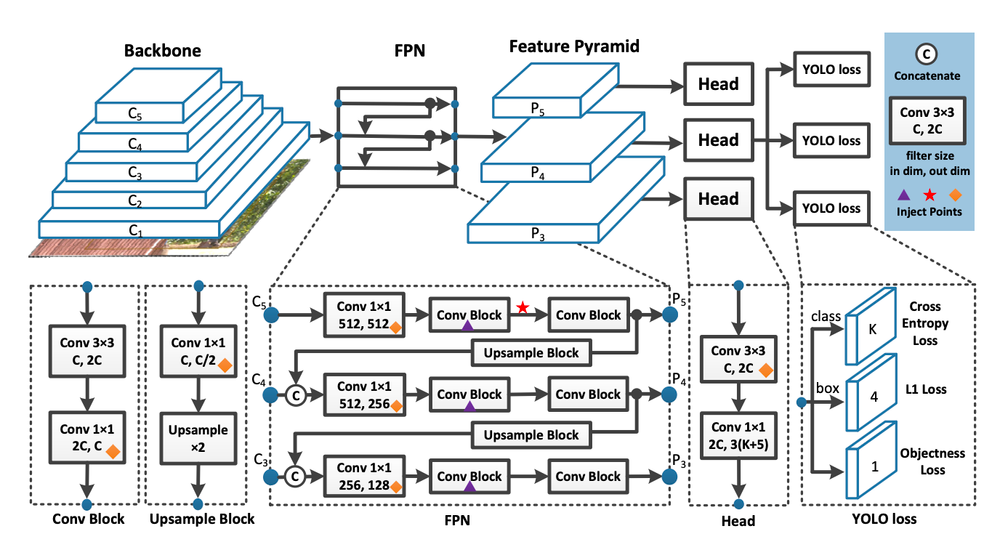
\includegraphics[width=\textwidth]{src/images/figures/yolov7_architecture.png}
    \caption{Architecture of YOLOv7}
    \label{fig:yolov7-architecture}
\end{figure}

The architecture of the YOLOv7 model is composed of three primary modules: Backbone, Neck, and Head.

\begin{itemize}
    \item \textbf{Backbone:} YOLOv7 uses an extended version of \gls{elan} (Efficient Layer Aggregation Network) as its backbone. This structure enables deeper network designs without significantly increasing computational cost. The backbone is responsible for extracting hierarchical features from the input image while preserving gradient flow and feature reuse.
    
    \item \textbf{Neck:} The neck in YOLOv7 incorporates a Path Aggregation Network (\gls{pan}) and ELAN-W modules. PAN enhances feature fusion across different scales, improving detection accuracy for both small and large objects. ELAN-W further refines spatial and contextual information during feature aggregation.
    
    \item \textbf{Head:} The head predicts object classes, bounding box coordinates $(x,y,h,w)$, and objectness scores. YOLOv7 uses a decoupled head, which separates classification and regression branches for better convergence and performance. The model outputs predictions at multiple scales to capture objects of varying sizes.
\end{itemize}

Further features of the model are as follows:

\begin{itemize}
    \item \textbf{Bounding Box Prediction:} The prediction of bounding box coordinates in YOLOv7 is guided by anchor-based regression, where the final bounding box $B=(x,y,w,h)$ is computed relative to the anchor box using the following formula:
    
    \begin{equation}
    x = \sigma(t_x) + c_x
    \label{eq:bbox-x}
    \end{equation}
    
    \begin{equation}
    y = \sigma(t_y) + c_y
    \label{eq:bbox-y}
    \end{equation}
    
    \begin{equation}
    w = p_w \cdot e^{t_w}
    \label{eq:bbox-w}
    \end{equation}
    
    \begin{equation}
    h = p_h \cdot e^{t_h}
    \label{eq:bbox-h}
    \end{equation}
    
    where $(t_x, t_y, t_w, t_h)$ are the predicted offsets, $(c_x, c_y)$ is the top-left corner of the grid cell, and $(p_w, p_h)$ are the dimensions of the anchor box.
    
    \item \textbf{Training Enhancements:} YOLOv7 introduces Coarse-to-Fine Lead Head, Model Scaling, and Auxiliary Heads that help improve gradient flow and stability during training. It supports Label Assignment Strategies such as dynamic-k matching for optimal anchor-label association.
    
    \item \textbf{Data Augmentation:} YOLOv7 applies automatic data augmentation during training including mosaic augmentation (combining four images into one), \gls{hsv} color augmentation, and random flipping, cropping, and scaling. These help increase dataset diversity and improve generalization.
    
    \item \textbf{Early Stopping and Training Stability:} YOLOv7 supports built-in early stopping based on a patience threshold if validation loss (combining box loss, objectness loss, and classification loss) does not improve for several epochs. This ensures faster convergence and prevents overfitting.
\end{itemize}

\subsection{Recognition of Component Values}

In order to generate a complete and simulation-ready netlist, it is essential to not only detect the components themselves but also to extract their associated parameter values, which are generally annotated near the components in the circuit diagram. Thus, it becomes essential to integrate Optical Character Recognition (\gls{ocr}) with the object detection pipeline to extract and map these values correctly to the corresponding components.

This involves identifying regions within the circuit image that likely contain text (done by YOLOv7), and then recognizing said texts in order to parse the component values along with their units.

The hand-written text recognition is done using a \gls{crnn}-based \gls{ocr} system, following the design philosophy of Deep Text Recognition Benchmark (DTRB) framework, however minor changes deemed suitable for this project have been made to get the text detection and recognition pipeline.

\begin{figure}[H]
    \centering
    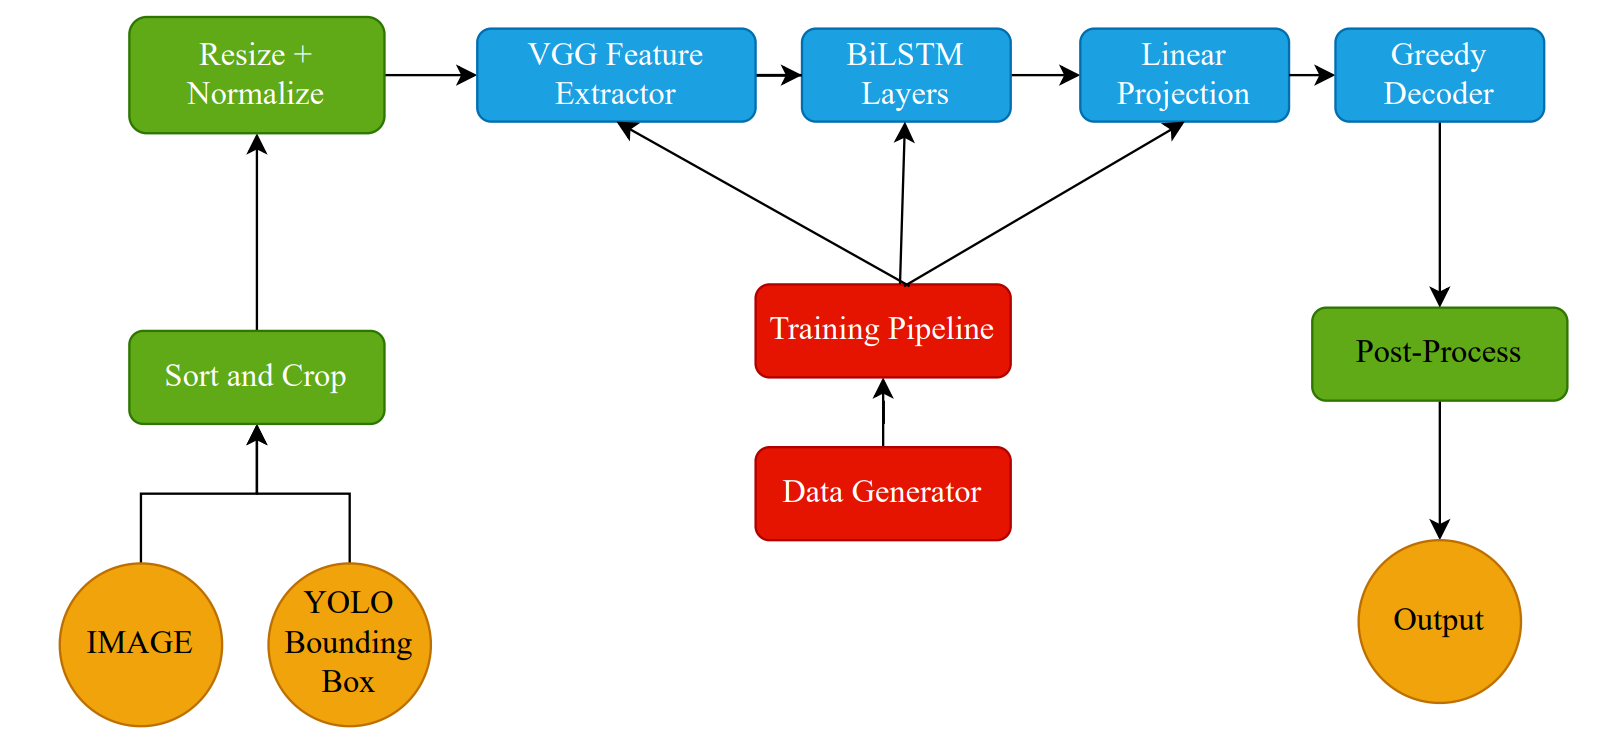
\includegraphics[width=\textwidth]{src/images/figures/easyocr_architecture.png}
    \caption{Text Detection and Recognition Pipeline}
    \label{fig:text-recognition-pipeline}
\end{figure}

YOLOv7 outputs (bounding box information) help segregate textual information (class `0' in the used dataset) which are then cropped, resized (to image height as 32) and normalized for compatibility with text recognition module. This is then passed through to a \gls{crnn} architecture composed of a Convolutional Encoder, Sequence Modeling Engine with Linear Projection, and \gls{ctc} Decoder.

\textbf{Convolutional Encoder (CNN):} A \gls{cnn} stack (e.g., VGG) transforms input image $I$ from multi-dimensional $\mathbb{R}^{H \times W \times C}$ to feature maps:

\begin{equation}
F = f_{\text{CNN}}(I_i), \quad F \in \mathbb{R}^{H' \times W' \times C}
\label{eq:cnn-encoder}
\end{equation}

\textbf{Sequence Modeling (Bidirectional LSTM):} Each $F$ becomes input to a bidirectional \gls{lstm}, yielding hidden states $h_t$. These hidden states capture context across the text line, allowing modeling of character sequences:

\begin{equation}
\overrightarrow{h_t} = \text{LSTM}_f(F_t, \overrightarrow{h_{t-1}})
\label{eq:bilstm}
\end{equation}

\textbf{CTC Decoder:} A softmax layer projects $h_t$ over the character vocabulary as:

\begin{equation}
p_{t,k} = \frac{e^{W_k h_t + b_k}}{\sum_{k'} e^{W_{k'} h_t + b_{k'}}}
\label{eq:ctc-softmax}
\end{equation}

The probability of sequence $z$ is computed over all alignments:

\begin{equation}
P(z \mid y) = \sum_{\pi: B(\pi)=z} \prod_{t=1}^{T} p_{t,\pi_t}
\label{eq:ctc-probability}
\end{equation}

The \gls{ctc} loss is given by the negative logarithm of $P(z \mid y)$. It enables end-to-end sequence decoding without explicit character bounding boxes.

During inference, greedy decoding strategy is used which selects the most-probable character at each time step while removing blank symbols and collapsing consecutive duplicate characters. The recognized text then needs to be mapped to the appropriate circuit component whose value it represents.

\subsection{Wire Detection}

Wire detection is performed using junction points detected by the object detection model as structural anchors for circuit connectivity. All detected junctions are first transformed from normalized detection space to pixel coordinates to ensure geometric consistency within the image domain. Pairwise combinations of junction points are then analyzed to identify potential wire candidates.

For each junction pair, a displacement vector and its orientation angle are computed. Based on a predefined angular tolerance, only near horizontal and near vertical orientations are retained, while diagonal connections are rejected to conform with standard schematic drawing conventions. Valid pairs are projected onto strict axis-aligned representations to form candidate wire segments.

To improve robustness against detection noise, wire endpoints are snapped to a uniform grid and collinear segments are consolidated using proximity and overlap criteria. This produces a compact and topologically consistent set of horizontal and vertical wire segments that represent the underlying circuit wiring.

\subsection{Terminal Point Detection}

Terminal point detection focuses on identifying meaningful electrical connection points associated with wires and components. Junction detections from the object detection model serve as primary terminal candidates, representing wire endpoints, intersections, and branching locations.

Once the final wire set is established, terminal points are refined by analyzing intersections between axis-aligned wire segments and component bounding boxes. Each intersection corresponds to a valid electrical terminal where a wire connects to a component edge. Intersection conditions are evaluated analytically to ensure precise localization of entry and exit points.

The resulting terminal points form a complete connectivity interface between wires and components, enabling accurate circuit graph construction and frontend mapping. This structured representation supports subsequent tasks such as netlist generation, interactive visualization, and automated circuit understanding.

\subsection{Integration Algorithm}

From the individual outputs from each of the aforementioned modules, the task is now to generate a structured \gls{json} representation of the circuit which will be used to generate a corresponding \gls{spice} netlist and also contribute in the schematic generation further down the line.

The integration between all these different outputs, in a simplistic form, would consist of the following steps:

\begin{itemize}
    \item Get a list of components and their corresponding bounding box coordinates (from YOLOv7).
    
    \item Get a list of text data and their corresponding bounding box coordinates (from \gls{ocr}).
    
    \item Map the component to the corresponding component value (text) based on the minimum Euclidean distance between a particular component and texts on the circuit.
    
    \item Once the terminals are determined based on the bounding boxes, match those terminal points to the nearest nodes in the circuit.
    
    \item Store the accumulated information in a \gls{json} file.
\end{itemize}

\subsection{SPICE Netlist Generation}

A netlist is a file that describes the connections between components in an electronic circuit. It acts as a blueprint, specifying which components are connected and how, without detailing the physical layout or specific component placement.

A \gls{spice} netlist is a text-based representation of an electrical circuit used for simulation by a \gls{spice} engine. It provides all the necessary information about the components, their connections, and their electrical properties, enabling analysis such as transient response, DC/AC sweep, or frequency domain behavior.

The netlist serves as input to a circuit simulation engine (NgSpice), which then performs numerical computations to evaluate how the circuit behaves under specified conditions.

For each component, the \gls{spice} netlist contains the information about its name, the nodes it is connected to on either side and the component's parameters or model (if necessary) in the following format:

\begin{center}
\texttt{<Component\_Name> <Node1> <Node2> <Value>}
\end{center}

After the \gls{json} file with abundant information about the components, their values, and the nodes they are connected to is generated, the next step is to convert said \gls{json} file into a netlist format (a \texttt{.txt} file which follows the appropriate conventions).

\subsection{Digital Schematic Generation}

The \gls{json} file built by integrating all the information about the hand-drawn circuit is to be manipulated through different JavaScript libraries to generate a digital, editable schematic of the circuit. As briefly discussed in the Requirements section, Chart.js is to be used to map each component in \gls{json} to a visual block (a symbol for the component as given by the KiCad symbol library). For each component, a graphical symbol needs to be rendered at a certain position and connection lines need to be drawn between the terminals and node positions. A rough pseudocode for the same is as follows:

\begin{algorithm}
\caption{Frontend Circuit Rendering}
\label{algo:frontend-rendering}
\begin{algorithmic}
\Require Circuit \gls{json} description $J$
\Ensure Rendered circuit schematic
\For{all component $c \in J.\text{components}$}
    \State Draw schematic symbol of type $c.\text{type}$ at position $c.\text{position}$
    \State Attach text label $c.\text{value}$ near component position
\EndFor
\For{all connection $k \in J.\text{connections}$}
    \State Retrieve terminal position from $k.\text{from}$ and terminal index
    \State Retrieve node position from $k.\text{node}$
    \State Draw wire between terminal and node positions
\EndFor
\State \Return Rendered schematic
\end{algorithmic}
\end{algorithm}

In order to make the schematic editable, Chart.js allows for draggable elements using inbuilt functions like \texttt{onDrag}, transformation handles for resizing and rotating, with added functions (and work-arounds in some cases) for integration of editing features like editing component value, delete/add components, etc. Changes can be saved by updating the \gls{json} structure on every interaction.

\subsection{Backend Development}

The backend is to be constructed using Next.js and FastAPI, functioning as the core middleware responsible for routing, processing, and orchestrating the system's \gls{ml} pipeline and user interactions. All endpoints follow a RESTful \gls{api} design, ensuring stateless and scalable communication between the frontend and the server.

Upon receiving a hand-drawn circuit image through an \gls{api} endpoint like \texttt{/upload}, the image is saved to a temporary storage location. The server invokes the YOLOv7 model (via a Python subprocess or containerized inference \gls{api}) to detect and localize electrical components. Simultaneously, the \gls{ocr} model is invoked to extract nearby textual annotations. The result is a list of components with bounding boxes and a list of recognized texts, each with confidence scores and coordinates.

Support for user interaction with the schematic is also handled by the backend. Operations such as component deletion, repositioning, wire addition, and modification of values are processed through specific \gls{api} endpoints. Each update is stored in the database, maintaining a real-time editable circuit representation. This allows the frontend to continuously reflect changes without direct manipulation of the database, ensuring security and stability of the system.

\subsection{LLM Integration}

To enhance interaction with the circuit beyond \gls{gui} manipulation, a large language model (\gls{llm}) is to be integrated, facilitated through LangChain and LangGraph. LangChain constructs the agent architecture responsible for handling user queries, such as, ``Explain the purpose of this resistor.'', ``Identify possible errors in this circuit.'', etc. The agent receives contextual data from the backend (such as the circuit's \gls{json} structure or \gls{spice} netlist), formats the prompt, and forwards it to the \gls{llm} through a secure \gls{api}. LangGraph manages the session state, context memory, and branching logic for multi-turn conversations. This enables the system to remember previously discussed components or simulation outputs across queries.

\section{Wire Detection Methodology}

The detection of wires in circuit diagrams requires a systematic approach that leverages geometric constraints inherent to electrical schematics. This section presents a comprehensive methodology for wire detection and terminal point analysis based on junction points detected by the YOLOv7 object detection framework. The fundamental assumption underlying this work is that circuit wires are predominantly axis-aligned, meaning they run either horizontally or vertically with respect to the image coordinate system.

The image domain is defined as the discrete set $\Omega = \{(x,y) \in \mathbb{Z} : 0 \le x < W, 0 \le y < H\}$ where $W$ and $H$ represent the image width and height in pixels respectively. The \gls{yolo} detection framework operates in a normalized coordinate space $\mathcal{U} = [0,1]^2$, necessitating a transformation to pixel coordinates for subsequent geometric analysis.

\subsection{Coordinate Denormalization}

The \gls{yolo} object detection framework produces detection tuples in normalized form. Each detection is represented as a quintuple $d = (c, x_n, y_n, w_n, h_n)$ where $c \in \mathbb{N}$ denotes the class label, $(x_n, y_n) \in [0,1]^2$ represents the normalized bounding box center, and $(w_n, h_n)$ specifies the normalized dimensions. For wire detection, only junction points are relevant, identified by class label $c = 1$.

The denormalization operator transforms normalized coordinates to pixel space through the affine map $\mathcal{N}^{-1} : \mathcal{U} \to \mathbb{R}^2$ defined as:

\begin{equation}
\mathcal{N}^{-1}(x_n, y_n) = \begin{pmatrix} W \cdot x_n \\ H \cdot y_n \end{pmatrix}
\label{eq:denormalization}
\end{equation}

This transformation constitutes a diagonal linear map with matrix representation $\text{diag}(W, H)$. The operator is bijective with determinant $WH \neq 0$, admitting the inverse $\mathcal{N}(x, y) = (x/W, y/H)$. The pixel-space junction set is thus constructed as $J = \{\mathbf{j} = \mathcal{N}^{-1}(x_n^{(d)}, y_n^{(d)}) : d \in \mathcal{J}\}$ where $\mathcal{J}$ denotes the subset of detections with class label unity.

\subsection{Pairwise Junction Analysis}

The wire detection algorithm operates by examining all possible pairs of junction points. For a junction set of cardinality $n = |J|$, the number of distinct unordered pairs requiring analysis is $\binom{n}{2} = n(n-1)/2$. Each pair $(\mathbf{j}_i, \mathbf{j}_k)$ with $i < k$ generates a displacement vector:

\begin{equation}
\mathbf{d}^{\leftrightarrow} = \mathbf{j}_k - \mathbf{j}_i = \begin{pmatrix} \Delta x \\ \Delta y \end{pmatrix}
\label{eq:displacement-vector}
\end{equation}

where $\Delta x = j_{k,x} - j_{i,x}$ and $\Delta y = j_{k,y} - j_{i,y}$ represent the horizontal and vertical displacements respectively. The magnitude of this displacement vector, given by $\|\mathbf{d}^{\leftrightarrow}\| = \sqrt{\Delta x^2 + \Delta y^2}$, represents the Euclidean distance between the junction pair.

\subsection{Angular Orientation Computation}

The orientation of the displacement vector is computed using the four-quadrant arctangent function, which correctly resolves the angle in all quadrants of the Cartesian plane. The signed orientation angle $\theta \in (-\pi, \pi]$ is defined as:

\begin{equation}
\theta = \text{atan2}(\Delta y, \Delta x)
\label{eq:angular-orientation}
\end{equation}

The \texttt{atan2} function is defined piecewise to handle all possible combinations of signs for its arguments. When $\Delta x > 0$, the angle equals $\arctan(\Delta y / \Delta x)$. When $\Delta x < 0$ and $\Delta y \ge 0$, a correction of $+\pi$ is applied. When $\Delta x < 0$ and $\Delta y < 0$, a correction of $-\pi$ is applied. The degenerate cases where $\Delta x = 0$ yield $\pm\pi/2$ depending on the sign of $\Delta y$.

For classification purposes, the angle is converted to a positive representation in degrees using the transformation $\tilde{\theta} = (180\theta / \pi) \mod 360$, yielding values in the range $[0^\circ, 360^\circ)$.

\subsection{Horizontal and Vertical Line Classification}

The classification of junction pairs as horizontal, vertical, or diagonal is accomplished through angular tolerance zones. The tolerance parameter $\epsilon = 18^\circ$ represents 10\% of the half-circle, providing sufficient margin to accommodate minor deviations from perfect alignment while maintaining classification accuracy.

\textbf{Horizontal Acceptance Region:} The set of angles classified as horizontal is defined as the union:

\begin{equation}
\Theta_H = [0^\circ, 18^\circ] \cup [162^\circ, 198^\circ] \cup [342^\circ, 360^\circ]
\label{eq:horizontal-region}
\end{equation}

This region captures angles within $\pm 18^\circ$ of the positive $x$-axis ($0^\circ$ and $360^\circ$) and within $\pm 18^\circ$ of the negative $x$-axis ($180^\circ$).

\textbf{Vertical Acceptance Region:} The set of angles classified as vertical is defined as:

\begin{equation}
\Theta_V = [72^\circ, 108^\circ] \cup [252^\circ, 288^\circ]
\label{eq:vertical-region}
\end{equation}

This region captures angles within $\pm 18^\circ$ of the positive $y$-axis ($90^\circ$) and within $\pm 18^\circ$ of the negative $y$-axis ($270^\circ$).

\textbf{Diagonal Rejection Region:} The complement of the horizontal and vertical regions constitutes the diagonal rejection region:

\begin{equation}
\Theta_D = [0^\circ, 360^\circ) \setminus (\Theta_H \cup \Theta_V)
\label{eq:diagonal-region}
\end{equation}

Junction pairs whose orientation falls within $\Theta_D$ are rejected as they do not represent valid axis-aligned wires.

The classification function $\mathcal{O} : [0^\circ, 360^\circ) \to \{H, V, \varnothing\}$ maps each angle to its corresponding orientation category. The total angular coverage of valid classifications is $(|\Theta_H| + |\Theta_V|)/360^\circ = 144^\circ/360^\circ = 40\%$, indicating that 40\% of angular space is accepted as orthogonal while 60\% is rejected as diagonal.

\subsection{Orthogonal Projection and Axis Alignment}

For junction pairs with valid orthogonal classification, the detected endpoints must be projected onto perfectly axis-aligned lines to ensure strict horizontal or vertical wire representation. This projection compensates for minor deviations from perfect alignment that fall within the tolerance zone.

\textbf{Horizontal Wire Projection:} For a junction pair $(\mathbf{j}_i, \mathbf{j}_k)$ with classification $\mathcal{O}(\tilde{\theta}) = \text{HORIZONTAL}$, the aligned wire is constructed by computing the mean $y$-coordinate:

\begin{equation}
\bar{y} = \frac{j_{i,y} + j_{k,y}}{2}
\label{eq:horizontal-projection}
\end{equation}

The projected wire endpoints are then defined as $\mathbf{s} = (j_{i,x}, \bar{y})$ and $\mathbf{e} = (j_{k,x}, \bar{y})$. Both endpoints share the same $y$-coordinate, ensuring perfect horizontal alignment.

\textbf{Vertical Wire Projection:} For a junction pair with classification $\mathcal{O}(\tilde{\theta}) = \text{VERTICAL}$, the aligned wire is constructed by computing the mean $x$-coordinate:

\begin{equation}
\bar{x} = \frac{j_{i,x} + j_{k,x}}{2}
\label{eq:vertical-projection}
\end{equation}

The projected wire endpoints are $\mathbf{s} = (\bar{x}, j_{i,y})$ and $\mathbf{e} = (\bar{x}, j_{k,y})$. Both endpoints share the same $x$-coordinate, ensuring perfect vertical alignment.

\textbf{Projection Error Bound:} For a junction pair with orientation angle $\tilde{\theta} \in [0^\circ, \epsilon]$ and inter-junction distance $L = \|\mathbf{d}^{\leftrightarrow}\|$, the maximum perpendicular displacement of any endpoint from its original position is bounded by:

\begin{equation}
\delta = \frac{|\Delta y|}{2} \le \frac{L \sin(\epsilon)}{2}
\label{eq:projection-error}
\end{equation}

For the tolerance $\epsilon = 18^\circ$ with $\sin(18^\circ) \approx 0.309$, this yields $\delta \approx 0.155L$. Thus, for a 100-pixel wire, the maximum projection displacement is approximately 15.5 pixels.

\subsection{Grid Quantization}

To ensure coordinate consistency and facilitate subsequent merging operations, all wire endpoints are quantized to a uniform grid. The grid structure is defined by the integer lattice $\mathcal{G} = g\mathbb{Z} \times g\mathbb{Z}$ where $g \in \mathbb{N}^+$ is the grid resolution, set to $g = 16$ pixels in this implementation.

\textbf{Snap Function:} The scalar quantization operator $\text{snap} : \mathbb{R} \to g\mathbb{Z}$ is defined as:

\begin{equation}
\text{snap}(v) = g \cdot \text{round}\left(\frac{v}{g}\right) = g \cdot \left\lfloor \frac{v}{g} + \frac{1}{2} \right\rfloor
\label{eq:snap-function}
\end{equation}

The vectorized extension $\text{Snap} : \mathbb{R}^2 \to \mathcal{G}$ applies the scalar operator component-wise, yielding $\text{Snap}(\mathbf{p}) = (\text{snap}(p_x), \text{snap}(p_y))$.

\textbf{Quantization Error Bounds:} For any scalar value $v \in \mathbb{R}$, the quantization error satisfies $|v - \text{snap}(v)| \le g/2$. For any vector $\mathbf{p} \in \mathbb{R}^2$, the error bounds are:

\begin{equation}
\|\mathbf{p} - \text{Snap}(\mathbf{p})\|_\infty \le \frac{g}{2}, \quad \|\mathbf{p} - \text{Snap}(\mathbf{p})\|_2 \le \frac{g\sqrt{2}}{2}
\label{eq:quantization-error}
\end{equation}

For $g = 16$ pixels, the maximum coordinate error is 8 pixels and the maximum Euclidean error is approximately 11.3 pixels.

\subsection{Wire Segment Consolidation}

The pairwise analysis of junctions frequently generates multiple overlapping wire segments that represent the same physical wire. The consolidation algorithm merges collinear segments within a tolerance threshold to produce a minimal set of non-redundant wires.

\textbf{Canonical Axis-Aligned Representation:} Each wire segment is transformed to a canonical form $\sigma = (a, \ell_{\min}, \ell_{\max}, \omega)$ where $a$ denotes the fixed axis coordinate ($y$-coordinate for horizontal wires, $x$-coordinate for vertical wires), $[\ell_{\min}, \ell_{\max}]$ specifies the extent along the variable axis, and $\omega \in \{H, V\}$ indicates the orientation.

For a horizontal wire $w = (\mathbf{s}, \mathbf{e}, H)$, the canonical form is $\sigma(w) = (s_y, \min(s_x, e_x), \max(s_x, e_x), H)$. For a vertical wire, the transformation is $\sigma(w) = (s_x, \min(s_y, e_y), \max(s_y, e_y), V)$. The segment length is defined as $L(\sigma) = \ell_{\max} - \ell_{\min}$.

\textbf{Mergeability Relation:} Two segments $\sigma_1$ and $\sigma_2$ with identical orientation are mergeable, denoted $\sigma_1 \sim \sigma_2$, if and only if:

\begin{equation}
|a_1 - a_2| \le \tau \land \ell_{\min}(\sigma_2) \le \ell_{\max}(\sigma_1) + \tau
\label{eq:mergeability}
\end{equation}

where $\tau = g$ is the grid tolerance and the segments are ordered such that $\ell_{\min}(\sigma_1) \le \ell_{\min}(\sigma_2)$. The first condition ensures proximity along the fixed axis, while the second condition requires overlap or near-touching along the variable axis.

\textbf{Merge Operator:} For mergeable segments $\sigma_1 \sim \sigma_2$, the merge operation produces a consolidated segment $\sigma_1 \oplus \sigma_2 = (a_{\text{merged}}, \ell_{\text{merged,min}}, \ell_{\text{merged,max}}, \omega)$ where:

\begin{equation}
a_{\text{merged}} = \begin{cases} a_1 & \text{if } L(\sigma_1) > L(\sigma_2) \\ a_2 & \text{otherwise} \end{cases}
\label{eq:merge-axis}
\end{equation}

\begin{equation}
\ell_{\text{merged,min}} = \min(\ell_{\min}(\sigma_1), \ell_{\min}(\sigma_2)), \quad \ell_{\text{merged,max}} = \max(\ell_{\max}(\sigma_1), \ell_{\max}(\sigma_2))
\label{eq:merge-extent}
\end{equation}

The length-weighted axis selection preserves the axis coordinate of the longer segment, which is assumed to be more geometrically accurate. The extent bounds are computed as the union of the individual extents.

\textbf{Merge Monotonicity:} The merge operation is length-non-decreasing, satisfying:

\begin{equation}
L(\sigma_1 \oplus \sigma_2) \ge \max(L(\sigma_1), L(\sigma_2))
\label{eq:merge-monotonicity}
\end{equation}

The proof follows from the observation that $L(\sigma_1 \oplus \sigma_2) = \max(\ell_{\max}(\sigma_1), \ell_{\max}(\sigma_2)) - \min(\ell_{\min}(\sigma_1), \ell_{\min}(\sigma_2))$. In the containment case where one segment contains the other, the merged length equals the longer segment. In the overlapping case, the merged length exceeds both individual lengths.

The consolidation algorithm proceeds by first separating segments by orientation, then sorting each group by axis coordinate and extent minimum. A linear scan merges consecutive mergeable segments, producing the final consolidated wire set.

\section{Terminal Detection}

Terminal detection refers to the identification of connection points between wire segments and circuit components. These intersection points are critical for establishing the circuit topology and enabling subsequent netlist extraction. This section presents the mathematical framework for detecting wire-component intersections based on axis-aligned bounding box geometry.

\subsection{Component Bounding Box Representation}

Circuit components detected by YOLOv7 are represented as axis-aligned bounding boxes (AABBs). For a detection tuple $d = (c, x_n, y_n, w_n, h_n)$ where $c \notin \{0, 1\}$ (excluding text and junction classes), the pixel-space bounding box is defined as:

\begin{equation}
\mathcal{B} = [x_{\min}, x_{\max}] \times [y_{\min}, y_{\max}]
\label{eq:bounding-box}
\end{equation}

The corner coordinates are computed from the normalized detection parameters as:

\begin{equation}
x_{\min} = \left(x_n - \frac{w_n}{2}\right) W, \quad x_{\max} = \left(x_n + \frac{w_n}{2}\right) W
\end{equation}

\begin{equation}
y_{\min} = \left(y_n - \frac{h_n}{2}\right) H, \quad y_{\max} = \left(y_n + \frac{h_n}{2}\right) H
\label{eq:box-corners}
\end{equation}

The boundary of the bounding box $\partial \mathcal{B}$ consists of four edges: the left edge at $x = x_{\min}$, the right edge at $x = x_{\max}$, the top edge at $y = y_{\min}$, and the bottom edge at $y = y_{\max}$.

\subsection{Wire Component Intersection Analysis}

Consolidated wire segments are represented in parametric form for intersection analysis. A horizontal wire with $y$-coordinate $y_w$ and $x$-extent $[x_{\min}, x_{\max}]$ defines the line segment:

\begin{equation}
\mathcal{L}_H = \{(x, y_w) : x \in [x_{\min}, x_{\max}]\}
\label{eq:horizontal-wire}
\end{equation}

Similarly, a vertical wire with $x$-coordinate $x_w$ and $y$-extent $[y_{\min}, y_{\max}]$ defines:

\begin{equation}
\mathcal{L}_V = \{(x_w, y) : y \in [y_{\min}, y_{\max}]\}
\label{eq:vertical-wire}
\end{equation}

\subsection{Horizontal Wire Intersection Conditions}

The intersection of a horizontal wire with a component bounding box can occur at either the left edge or the right edge of the box. The intersection conditions are derived from the geometric constraints of axis-aligned segments.

\textbf{Horizontal Wire–Left Edge Intersection:} The horizontal wire $\mathcal{L}_H$ with parameters $(y_w, x_{\min}, x_{\max})$ intersects the left edge of bounding box $\mathcal{B} = [x_{\min}, x_{\max}] \times [y_{\min}, y_{\max}]$ at point $(x_{\min}, y_w)$ if and only if:

\begin{equation}
\Phi_L(\mathcal{L}_H, \mathcal{B}) = (y_{\min} \le y_w \le y_{\max}) \land (x_{\min} \le x_{\min} \le x_{\max})
\label{eq:horizontal-left-intersection}
\end{equation}

The first condition $(y_{\min} \le y_w \le y_{\max})$ ensures vertical alignment, requiring that the wire's $y$-coordinate falls within the vertical extent of the box. The second condition $(x_{\min} \le x_{\min} \le x_{\max})$ ensures horizontal overlap, requiring that the left edge $x$-coordinate falls within the horizontal extent of the wire.

The proof of necessity follows from the observation that if an intersection exists at $(x_{\min}, y_w)$, then this point must simultaneously lie on the wire (requiring $y = y_w$ and $x \in [x_{\min}, x_{\max}]$) and on the left edge (requiring $x = x_{\min}$ and $y \in [y_{\min}, y_{\max}]$). Sufficiency is established by verifying that when both conditions hold, the point $(x_{\min}, y_w)$ belongs to both the wire segment and the box boundary.

\textbf{Horizontal Wire–Right Edge Intersection:} The horizontal wire $\mathcal{L}_H$ intersects the right edge of $\mathcal{B}$ at point $(x_{\max}, y_w)$ if and only if:

\begin{equation}
\Phi_R(\mathcal{L}_H, \mathcal{B}) = (y_{\min} \le y_w \le y_{\max}) \land (x_{\min} \le x_{\max} \le x_{\max})
\label{eq:horizontal-right-intersection}
\end{equation}

The structure mirrors that of the left edge intersection, with $x_{\max}$ replacing $x_{\min}$ in the horizontal overlap condition.

\subsection{Vertical Wire Intersection Conditions}

The intersection of a vertical wire with a component bounding box can occur at either the top edge or the bottom edge of the box.

\textbf{Vertical Wire–Top Edge Intersection:} The vertical wire $\mathcal{L}_V$ with parameters $(x_w, y_{\min}, y_{\max})$ intersects the top edge of bounding box $\mathcal{B}$ at point $(x_w, y_{\min})$ if and only if:

\begin{equation}
\Phi_T(\mathcal{L}_V, \mathcal{B}) = (x_{\min} \le x_w \le x_{\max}) \land (y_{\min} \le y_{\min} \le y_{\max})
\label{eq:vertical-top-intersection}
\end{equation}

The first condition $(x_{\min} \le x_w \le x_{\max})$ ensures horizontal alignment, requiring that the wire's $x$-coordinate falls within the horizontal extent of the box. The second condition $(y_{\min} \le y_{\min} \le y_{\max})$ ensures vertical overlap, requiring that the top edge $y$-coordinate falls within the vertical extent of the wire.

\textbf{Vertical Wire–Bottom Edge Intersection:} The vertical wire $\mathcal{L}_V$ intersects the bottom edge of $\mathcal{B}$ at point $(x_w, y_{\max})$ if and only if:

\begin{equation}
\Phi_B(\mathcal{L}_V, \mathcal{B}) = (x_{\min} \le x_w \le x_{\max}) \land (y_{\min} \le y_{\max} \le y_{\max})
\label{eq:vertical-bottom-intersection}
\end{equation}

\subsection{Complete Intersection Set Construction}

The intersection set for a single wire-box pair aggregates all valid intersections across the relevant edges.

\textbf{Wire-Box Intersection Set:} For wire $w$ with orientation $\omega$ and bounding box $\mathcal{B}$, the intersection set is defined as:

\begin{equation}
\mathcal{I}(w, \mathcal{B}) = \begin{cases}
\{(x_{\min}, y_w) : \Phi_L\} \cup \{(x_{\max}, y_w) : \Phi_R\} & \text{if } \omega = H \\
\{(x_w, y_{\min}) : \Phi_T\} \cup \{(x_w, y_{\max}) : \Phi_B\} & \text{if } \omega = V
\end{cases}
\label{eq:wire-box-intersection-set}
\end{equation}

\textbf{Intersection Cardinality Bound:} For each wire-box pair, the cardinality of the intersection set is bounded by $|\mathcal{I}(w, \mathcal{B})| \le 2$. This bound reflects the geometric reality that a straight axis-aligned wire can enter a rectangular box through one edge and exit through the opposite edge, yielding at most two intersection points.

The global intersection set aggregates all wire-box intersections across the complete wire set $\mathcal{W}$ and component box set $\mathcal{C}$:

\begin{equation}
\mathcal{I}_{\text{total}} = \bigcup_{w \in \mathcal{W}} \bigcup_{\mathcal{B} \in \mathcal{C}} \mathcal{I}(w, \mathcal{B})
\label{eq:global-intersection-set}
\end{equation}

\subsection{Terminal Point Significance}

The detected intersection points serve as terminal connection points in the circuit topology. Each intersection $(x, y) \in \mathcal{I}_{\text{total}}$ indicates a location where a wire connects to a component, enabling the construction of a circuit graph where components are nodes and wires are edges. This representation facilitates subsequent circuit analysis tasks including netlist generation, connectivity verification, and schematic reconstruction.

\section{Use-Case Diagram}

The use-case diagram in Figure~\ref{fig:use-case-diagram} outlines the CIRCUITRON system's functionality depicting the interactions between users and the system. The primary actor is the user, who can be a student, instructor, or engineer. The system begins with the user uploading a hand-drawn circuit image.

Upon submission, CIRCUITRON automatically preprocesses the image to enhance clarity and prepares it for further analysis. The system then detects components (e.g., resistors, capacitors) using YOLOv7 and identifies wires and nodes through techniques like junction-based wire detection. Simultaneously, it extracts text labels (e.g., component values) using \gls{ocr} and maps them to the corresponding components.

Once the circuit structure is parsed, the system generates an editable schematic, allowing the user to manually correct any errors before proceeding. After validation, the system converts the schematic into a SPICE-compatible netlist and runs a simulation using Ngspice/PySpice. The results, including voltage and current graphs, are displayed to the user. Additionally, the system integrates an AI assistant to answer circuit-related questions, enhancing the learning and troubleshooting experience.

The ``includes'' relationship is used for mandatory sub-tasks like component detection and \gls{ocr}, which must always execute as part of core workflows. The ``extends'' relationship marks optional features like manual corrections or AI Q\&A, which enhance functionality but aren't required for basic operation. The diagram effectively outlines the system's scope, emphasizing its applications (or use-cases).

\begin{figure}[H]
    \centering
     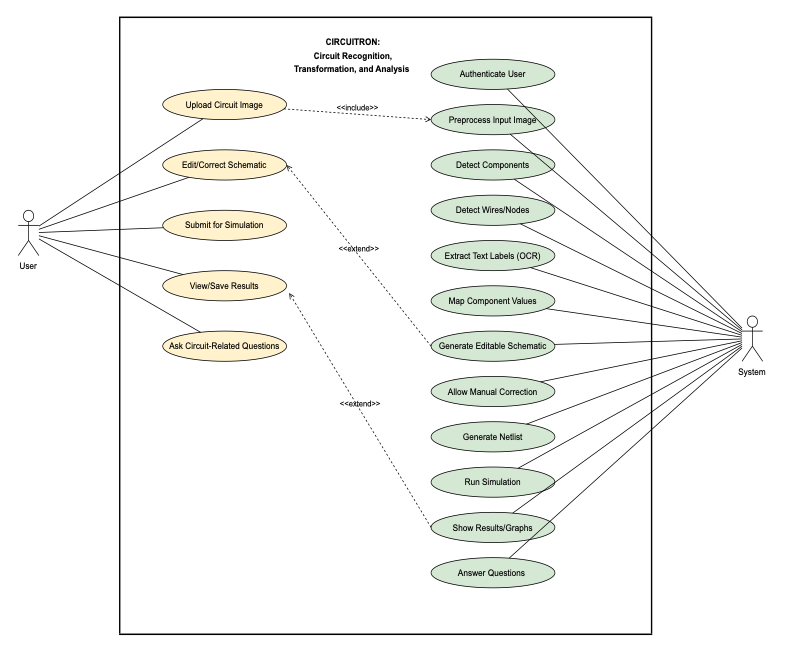
\includegraphics[width=\textwidth]{src/images/figures/use_case_diagram.png}
    \caption{Use-Case Diagram for CIRCUITRON System}
    \label{fig:use-case-diagram}
\end{figure}

\section{Performance Metrics Expectation}

No matter how rigorously the models are trained and fine-tuned, there is always room for error due to edge cases like unclear handwriting and similar-looking components. As such, for any project, it is important to define appropriate performance metrics which indicate when the models can be considered ``good-enough'' for the required purpose. Table~\ref{table:performance-metrics} shows the chosen performance metrics and their target values on achieving which, the training may be stopped.

\begin{table}[H]
    \centering
    \caption{Expected Performance Metric Values for Individual Modules}
    \label{table:performance-metrics}
    \begin{tabular}{lcc}
        \toprule
        \textbf{Pipeline Stage} & \textbf{Performance Metric} & \textbf{Target Value/Expectation} \\
        \midrule
        Component Detection & mAP@0.5 & 0.90 \\
        Text Recognition & Character Accuracy & 0.75 \\
        \bottomrule
    \end{tabular}
\end{table}

\subsection{Component Detection Metric}

mAP@0.5 (mean Average Precision at IoU threshold of 0.5) evaluates how well the model detects components with correct class labels and bounding boxes. It calculates the Average Precision (\gls{ap}) for each class and then takes the mean across all classes. An \gls{iou} (Intersection over Union) threshold of 0.5 means a predicted bounding box is considered a correct match if it overlaps with the ground truth box by at least 50\%.

\begin{equation}
\text{IoU} = \frac{\text{Area of Overlap}}{\text{Area of Union}}
\label{eq:iou-metric}
\end{equation}

A high mAP@0.5 means detections are both precise and complete, minimizing missed or misclassified components.

\subsection{Text Recognition Metric}

Character Accuracy measures how many characters in the predicted text match the actual characters:

\begin{equation}
\text{Character Accuracy} = \frac{\text{Number of Correct Characters}}{\text{Total Number of Characters in Ground Truth}}
\label{eq:character-accuracy}
\end{equation}

In circuit diagrams, values like $10k$, $100\Omega$, $1\mu F$ are crucial. \gls{ocr} must correctly read these values, since even a small error (e.g., mistaking `k' as `1') leads to incorrect simulation behavior. A high character accuracy ensures value-to-component mapping is reliable.

\subsection{Terminal and Node Detection Metrics}

Precision measures how many detected terminals (or nodes) are correct whereas recall measures how many actual terminals (or nodes) were correctly detected:

\begin{equation}
\text{Precision} = \frac{\text{True Positives}}{\text{True Positives} + \text{False Positives}}
\label{eq:precision}
\end{equation}

\begin{equation}
\text{Recall} = \frac{\text{True Positives}}{\text{True Positives} + \text{False Negatives}}
\label{eq:recall}
\end{equation}

Terminals define where components connect to wires, which influences circuit structure. High precision ensures the system doesn't falsely identify noise as terminals, avoiding wrong wire mappings. High recall ensures the system doesn't miss valid terminal points, which would cause incomplete circuits. Likewise, missing nodes can create open circuits, and false nodes can misrepresent actual connectivity. So high values of both precision and recall are crucial for both terminal and node detection.

\section{Error Handling}

In any project with a number of individual modules working together, the overall error not only comes from said individual modules but also from their integration due to propagating errors from one module to another. To handle errors in such a case, foremost the errors in the output of the individual modules need to be controlled and only then can the accumulated error be kept in check. The performance metrics tabulated in the previous section are to be strictly adhered to if there's any hope of generating the \gls{spice} netlist (and digital schematic) with nominal errors.

For the reduction of false matches and \gls{ocr} noise, post-processing techniques such as value format validation, confidence filtering, and text cleanup can be implemented. Value format validation ensures only strings that match known (and appropriate) electrical units, say $10k$, $1\mu F$, $5V$ are retained. Confidence filtering helps discard \gls{ocr} results with low confidence scores, and text cleanup normalizes ambiguous symbols such as converting ``O'' to ``0'', ``$\mu$'' to ``u''.

A basic pseudocode for sample value format validation is as follows:

\begin{algorithm}
\caption{Validation and Filtering of OCR Component Values}
\label{algo:ocr-validation}
\begin{algorithmic}
\Require OCR detected text entries $T$
\Ensure Filtered list of valid component values $V$
\State Define regular expression patterns for resistance, capacitance, and voltage
\State $V \leftarrow \emptyset$
\For{all text entry $t \in T$}
    \If{$t.\text{text}$ matches any defined pattern}
        \State Append $t$ to $V$
    \EndIf
\EndFor
\State \Return $V$
\end{algorithmic}
\end{algorithm}

The list of components shown here is in no way meant to be exhaustive; rather it is to show how this pseudocode ensures that only valid electrical component values are used in the final component-to-value mapping and schematic generation.

To prevent propagating error (error from the output of YOLOv7 bleeding into \gls{ocr}, for instance), a combined confidence threshold checking mechanism can be implemented which marks an item as uncertain if the confidence score from YOLOv7 is less than a certain value (e.g., 0.6) and the same from \gls{ocr} is less than a certain value (e.g., 0.85). For more robustness, a human-in-the-loop mechanism can be implemented which prompts the user to manually approve or correct \gls{ocr}-predicted values, fix connection errors, etc. This can be implemented to trigger when the confidence score is below the set threshold or when other error handling mechanisms such as value format validation fail. The pseudocode for this is as follows:

\begin{algorithm}
\caption{Confidence-Based Error Checking and Validation}
\label{algo:confidence-validation}
\begin{algorithmic}
\Require Module outputs $O$, confidence threshold $\omega$, format validation function $f$
\Ensure Valid outputs $V$ and uncertain outputs $U$
\State $V \leftarrow \emptyset$
\State $U \leftarrow \emptyset$
\For{all item $o \in O$}
    \If{$o.\text{confidence} \ge \omega \land f(o.\text{value})$}
        \State Append $o$ to $V$
    \Else
        \State Append $o$ to $U$
    \EndIf
\EndFor
\If{$U \ne \emptyset$}
    \State Trigger manual override
\EndIf
\State \Return $(V, U)$
\end{algorithmic}
\end{algorithm}

\subsection{Image Augmentation}

Since the dataset contains handwritten circuit diagrams captured under variable lighting and orientations, several augmentation techniques were applied to improve model generalization including Contrast Enhancement (global) and Adaptive Brightness Adjustment by factors of 0.8 and 1.2. Furthermore, geometric augmentation techniques, like spatial flipping (both horizontally and vertically) and rotation (e.g., $90^\circ$ or random rotation) proved to be unwise operations for this project. For example, if a ``C'' is rotated by $90^\circ$, the ``C'' now resembles a ``U'', and the same applies to flipping (``M'' might look like ``W'', for example). Rather than increasing accuracy, it was realized that using rotation or flipping would simply confuse the model. However, continuous testing with other forms of augmentation will continue in hopes of improving the model.

\subsection{Fine-tuning YOLOv5 and YOLOv7 for Component Detection}

YOLOv5 was initially used for benchmarking, and later upgraded to YOLOv7 for better accuracy and inference speed (comparison shown in the Results section). Training and fine-tuning were done using the \gls{cghd} dataset after converting into \gls{yolo}-compatible format.

The training parameters employed are as follows:

\begin{itemize}
    \item \textbf{Number of classes:} 61
    \item \textbf{Training split:} 70\% training, 10\% validation, 20\% testing
    \item \textbf{Epochs:} 200 (for YOLOv5), 100 (for YOLOv7)
    \item \textbf{Image size:} $416 \times 416$ pixels
    \item \textbf{Batch size:} 16 (for YOLOv5), 32 (for YOLOv7)
    \item \textbf{Optimizer:} \gls{sgd} (Stochastic Gradient Descent)
    \item \textbf{Learning rate:} 0.01 (initial)
    \item \textbf{Augmentations used in training:} Mosaic Augmentation, \gls{hsv} Augmentation, Random rotating/flipping
\end{itemize}

\subsection{Implementation of Text Recognition (OCR)}

To extract textual information such as resistor values, capacitor labels, and other component annotations from the circuit diagrams, a \gls{crnn}-based custom \gls{ocr} model was chosen, trained and implemented. The input image in cropped form (cropped for each text component) was passed through this model after training, which returned the content of each detected text element. The position of said text element, however, was found using bounding boxes from YOLOv7. This allowed us to localize and read numerical values or labels directly from the circuit.

Three different modules, each for feature extraction, sequence modeling, and prediction were trained based on the DTRB framework. Initially, simply fine-tuning \gls{ocr} models like TrOCR and EasyOCR were also attempted; however, these didn't yield usable results, ultimately requiring training from scratch. The training was done for 29 epochs.

\subsection{Line Detection Algorithm Implementation}

The line detection mechanism was engineered to exploit the semantic constraints of circuit diagrams, specifically that wires are predominantly axis-aligned (horizontal or vertical) and connect distinct components. Unlike the Probabilistic Hough Transform (\gls{pht}) which operates purely on pixel gradients, this approach uses the junction points detected by YOLOv7 as anchor nodes to reconstruct the wiring layout geometrically.

First, a pairwise analysis was performed on all junction points identified by the object detection model. The algorithm iterates through every unique pair of junctions to calculate the angle of the vector connecting them. Since hand-drawn circuits contain imperfections, an angular tolerance of $\pm 18^\circ$ was applied to classify connections as either horizontal or vertical. To ensure coordinate consistency across the diagram, the resulting segment coordinates were ``snapped'' to a grid using a 16-pixel quantization.

\begin{algorithm}
\caption{Wire Classification and Alignment}
\label{algo:wire-classification}
\begin{algorithmic}
\Require Set of junctions $J$, angular tolerance $\omega_{\text{tol}} = 18^\circ$, grid size $g = 16$
\Ensure Set of raw wire segments $S$
\State $S \leftarrow \emptyset$
\For{all pairs $(j_a, j_b) \in \text{Combinations}(J, 2)$}
    \State $\Delta x \leftarrow j_b.x - j_a.x$
    \State $\Delta y \leftarrow j_b.y - j_a.y$
    \State $\theta \leftarrow \text{atan2}(\Delta y, \Delta x)$
    \If{$|\theta| \le \omega_{\text{tol}} \lor |\theta - 180^\circ| \le \omega_{\text{tol}}$}
        \State \textbf{Horizontal alignment check}
        \State $y_{\text{avg}} \leftarrow \frac{j_a.y + j_b.y}{2}$
        \State $y_{\text{snap}} \leftarrow \text{Round}\left(\frac{y_{\text{avg}}}{g}\right) \times g$
        \State $S \leftarrow S \cup \{(H, y_{\text{snap}}, \min(j_a.x, j_b.x), \max(j_a.x, j_b.x))\}$
    \ElsIf{$|\theta - 90^\circ| \le \omega_{\text{tol}} \lor |\theta - 270^\circ| \le \omega_{\text{tol}}$}
        \State \textbf{Vertical alignment check}
        \State $x_{\text{avg}} \leftarrow \frac{j_a.x + j_b.x}{2}$
        \State $x_{\text{snap}} \leftarrow \text{Round}\left(\frac{x_{\text{avg}}}{g}\right) \times g$
        \State $S \leftarrow S \cup \{(V, x_{\text{snap}}, \min(j_a.y, j_b.y), \max(j_a.y, j_b.y))\}$
    \EndIf
\EndFor
\State \Return $S$
\end{algorithmic}
\end{algorithm}

A common issue with the pairwise approach is the generation of redundant, overlapping segments for the same wire. For instance, if three junctions lie on a single line, the algorithm produces three separate segments (A-B, B-C, and A-C). To combat this, a collinear segment merging algorithm was implemented.

The segments were first separated by orientation (horizontal/vertical) and sorted by their primary axis. The merging logic then consolidated overlapping or adjacent segments. Crucially, a length-weighted heuristic was used: when merging, the axis coordinate of the longer segment was preserved, ensuring that larger, more reliable strokes dictated the final geometric alignment.

\begin{algorithm}
\caption{Collinear Segment Merging}
\label{algo:segment-merging}
\begin{algorithmic}
\Require List of segments $L$, gap tolerance $\omega$
\Ensure List of merged segments $M$
\State Sort $L$ by primary axis, then by starting coordinate
\State $M \leftarrow \emptyset$
\State $\text{curr} \leftarrow L[0]$
\For{all $\text{next} \in L[1 \ldots N]$}
    \If{$|\text{curr.axis} - \text{next.axis}| \le \omega \land \text{next.start} \le \text{curr.end} + \omega$}
        \State $\text{curr.start} \leftarrow \min(\text{curr.start}, \text{next.start})$
        \State $\text{curr.end} \leftarrow \max(\text{curr.end}, \text{next.end})$
        \If{$\text{Length}(\text{next}) > \text{Length}(\text{curr})$}
            \State \textbf{Preserve axis of the longer segment}
            \State $\text{curr.axis} \leftarrow \text{next.axis}$
        \EndIf
    \Else
        \State $M \leftarrow M \cup \{\text{curr}\}$
        \State $\text{curr} \leftarrow \text{next}$
    \EndIf
\EndFor
\State $M \leftarrow M \cup \{\text{curr}\}$
\State \Return $M$
\end{algorithmic}
\end{algorithm}

The wire–component intersection detection algorithm identifies precise connection points between detected wire segments and component bounding boxes. Component regions are first extracted from YOLOv7 annotations and converted into pixel coordinates. Each horizontal and vertical wire is then tested for geometric intersection with the edges of every component box. The resulting intersection points are used to accurately map circuit connectivity and are optionally visualized for verification in the frontend.

\begin{algorithm}
\caption{Wire–Component Intersection Detection}
\label{algo:wire-component-intersection}
\begin{algorithmic}
\Require Wire segments $W$, \gls{yolo} label file $L$, image width $I_w$, image height $I_h$
\Ensure Set of intersection points $P$
\State Parse label file $L$
\State Convert normalized bounding boxes to pixel coordinates
\State Discard non-component classes
\State Store component boxes $B$
\State \textbf{Detect intersections between wires and components}
\State $P \leftarrow \emptyset$
\For{all wire $w \in W$}
    \For{all box $b \in B$}
        \If{$w$ is horizontal and crosses left or right edge of $b$}
            \State Add intersection point to $P$
        \ElsIf{$w$ is vertical and crosses top or bottom edge of $b$}
            \State Add intersection point to $P$
        \EndIf
    \EndFor
\EndFor
\State Draw wires, component boxes, and intersection points on image
\State Save output visualization
\State \Return $P$
\end{algorithmic}
\end{algorithm}

While detecting terminals, a method to ensure faulty values are not accepted is to count the terminals. Unless a few three-terminal components are used, the number of terminals is likely to be even, so a mismatch in this could potentially indicate an error. In such cases, the detection can be re-run and/or the user can be notified. In case of failure to detect or associate a value, and if other error-handling mechanisms are not triggered, a placeholder can be used (e.g., $R1 = \text{UNKNOWN}$), and the system allows manual user correction before simulation as a last resort.

\section{System Flowchart}

\begin{figure}[H]
    \centering
    
\includegraphics[width=\textwidth]{src/images/figures/flowchart.png}
    \caption{System Flowchart}
    \label{fig:system-flowchart}
\end{figure}

The key architectural modules involved in the working of the system have been demonstrated by the block diagram in Figure~\ref{fig:block-diagram-circuitron}. Now, the flowchart in Figure~\ref{fig:system-flowchart} demonstrates the motions a user needs to go through to use the final product. First, the user needs to be authenticated (optional). Once the image of a hand-drawn circuit is uploaded, the system processes the image (internally using the techniques explained in the previous sections) and returns an editable schematic. Any necessary update or correction may be performed if necessary and then the schematic can be submitted for simulation and analysis. Relevant graphs are returned after analysis and the result can be saved for later access.

\section{Dataset Analysis}

In order to develop the system using the system for automated circuit diagram understanding, the \gls{cghd} (Circuit Graph Handwritten Diagrams) dataset is used. This dataset provides a comprehensive suite of ground truth annotations tailored to facilitate key computer vision tasks such as object detection, instance segmentation, and text recognition. While additional datasets (such as circuitVQA, Digitize-HCD datasets) may be used to fine-tune the models in the future to achieve even higher values for performance metrics, as of yet, only the \gls{cghd} dataset has been used.

\subsection{Dataset Overview}

The \gls{cghd} dataset comprises 4.99 GB of annotated data spanning over 3,000 raw images. The data is separated into folders named drafters, going from $-1$ through 31, and each drafter folder contains hand-sketches of 12 unique circuit designs, with each circuit drawn twice and captured under four different conditions (varying angles, lighting, and minor distortions), resulting in up to 96 images per drafter. As is convention, the dataset is to be split into (70-20-10)\% of the entire data for training, validation and testing respectively.

\begin{table}[H]
    \centering
    \caption{Summary of Data in the CGHD Dataset}
    \label{table:cghd-summary}
    \begin{tabular}{lr}
        \toprule
        \textbf{Items} & \textbf{Number} \\
        \midrule
        Distinct Circuits & 372 \\
        Raw Images & 3,269 \\
        Bounding Box Annotations & 248,020 \\
        Text String Annotations & 85,417 (93.74\% completeness) \\
        Character Types & 98 \\
        Object Classes & 61 \\
        \bottomrule
    \end{tabular}
\end{table}

Every image is rigorously annotated and the annotations provided per image include:

\begin{itemize}
    \item \textbf{Bounding Boxes (PASCAL VOC format)} for 61 electrical component classes, including resistors, capacitors, transistors, operational amplifiers, and textual elements.
    
    \item \textbf{Text Labels} capturing component values and identifiers (e.g., ``$10k\Omega$'', ``$C1$'', ``$V$'').
    
    \item \textbf{Instance Segmentation Polygons} (LabelMe JSON format) for pixel-level object outlines.
    
    \item \textbf{Binary Segmentation Maps} distinguishing foreground circuit strokes from background artifacts.
    
    \item \textbf{Partial Netlist Files} (in \texttt{.asc} format) for selected samples, useful for validating circuit reconstruction.
\end{itemize}

The text annotation coverage is extensive, with labels ranging from single characters (like ``$R$'' or ``$R1$'') to full descriptors (like ``Resistor'', ``Variable Resistor'', etc.).

\subsection{Class-wise Data Statistics}

\begin{table}[H]
    \centering
    \caption{Frequency of Each Class with its Code in the CGHD Dataset}
    \label{table:cghd-classes}
    \begin{tabular}{rll|rll}
        \toprule
        \textbf{Code} & \textbf{Class Name} & \textbf{Count} & \textbf{Code} & \textbf{Class Name} & \textbf{Count} \\
        \midrule
        1 & text & 91,122 & 32 & opamp.schmitt & 16 \\
        2 & junction & 79,202 & 33 & optocoupler & 162 \\
        3 & crossover & 10,180 & 34 & ic & 1,506 \\
        4 & terminal & 11,253 & 35 & ic.ne555 & 262 \\
        5 & gnd & 5,501 & 36 & ic.v\_regulator & 362 \\
        6 & vss & 1,354 & 37 & xor & 162 \\
        7 & voltage.dc & 335 & 38 & and & 860 \\
        8 & voltage.ac & 292 & 39 & or & 440 \\
        9 & voltage.battery & 765 & 40 & not & 496 \\
        10 & resistor & 14,400 & 41 & nand & 228 \\
        11 & resistor.adj & 1,052 & 42 & nor & 59 \\
        12 & resistor.photo & 65 & 43 & probe & 184 \\
        13 & cap.unpol & 5,841 & 44 & probe.curr & 72 \\
        14 & cap.pol & 2,227 & 45 & probe.volt & 32 \\
        15 & cap.adj & 88 & 46 & switch & 2,184 \\
        16 & inductor & 1,976 & 47 & relay & 89 \\
        17 & inductor.ferrite & 120 & 48 & socket & 184 \\
        18 & inductor.coupled & 10 & 49 & fuse & 226 \\
        19 & transformer & 483 & 50 & speaker & 410 \\
        20 & diode & 3,890 & 51 & motor & 108 \\
        21 & diode.led & 1,212 & 52 & lamp & 301 \\
        22 & diode.thyrector & 16 & 53 & microphone & 72 \\
        23 & diode.zener & 609 & 54 & antenna & 24 \\
        24 & diac & 40 & 55 & crystal & 112 \\
        25 & triac & 98 & 56 & mechanical & 32 \\
        26 & thyristor & 415 & 57 & magnetic & 364 \\
        27 & varistor & 184 & 58 & optical & 127 \\
        28 & transistor.bjt & 3,678 & 59 & block & 0 \\
        29 & transistor.fet & 977 & 60 & explanatory & 610 \\
        30 & transistor.photo & 177 & 61 & unknown & 32 \\
        31 & opamp & 752 &  &  &  \\
        \bottomrule
    \end{tabular}
\end{table}


\chapter{IMPLEMENTATION DETAILS}

The implementation of the system to convert hand-drawn circuit diagrams into simulation-ready netlists and digital schematics follows a modular approach, aligning with the pipeline described in the architecture and methodology. Some of the methodologies explained in the previous section, that have been implemented are explained in this section.

\section{Dataset Manipulation and Preprocessing}

\subsection{Conversion of Annotation Formats}

To accommodate the multiple models in the pipeline (YOLOv7 for component detection and \gls{ocr} for value extraction), annotation files provided in the \gls{cghd} dataset in Pascal VOC (XML) format were converted into compatible formats. Likewise, for EasyOCR-inspired custom-trained \gls{ocr}, all text-sections needed to be cropped out from the image with corresponding labels (ground truth) and then fed to the fine-tuned model.

In Pascal VOC format, the information regarding the circuit and its components are stored in the following format as shown by the example below:

\begin{lstlisting}[language=XML, frame=none, numbers=none, backgroundcolor=, basicstyle=\ttfamily\fontsize{12}{14}\selectfont, label={lst:pascal-voc-example}]
<annotation>
    <folder>images</folder>
    <filename>C1_D1_P2.jpg</filename>
    <path>./drafter_1/images/C1_D1_P2.jpg</path>
    <source>
        <database>CGHD</database>
    </source>
    <size>
        <width>3024</width>
        <height>4032</height>
        <depth>3</depth>
    </size>
    <segmented>0</segmented>
    <object>
        <name>voltage.dc</name>
        <pose>Unspecified</pose>
        <truncated>0</truncated>
        <difficult>0</difficult>
        <bndbox>
            <xmin>327</xmin>
            <ymin>546</ymin>
            <xmax>604</xmax>
            <ymax>838</ymax>
            <rotation>10</rotation>
        </bndbox>
    </object>
</annotation>
\end{lstlisting}

For \gls{yolo}-based detection, XML annotations were converted to \gls{yolo} format (\texttt{.txt}) using a custom \gls{python} script. Each \texttt{.txt} file contains the class index and normalized bounding box coordinates in the format:

\begin{center}
\texttt{<class\_id> <x\_center> <y\_center> <width> <height>}
\end{center}

The pseudocode for the VOC to YOLO annotation conversion is as follows:

\begin{algorithm}
\caption{VOC to YOLO Annotation Conversion}
\label{algo:voc-to-yolo}
\begin{algorithmic}
\Require XML annotation file $X$, class map $C$, image width $W$, image height $H$
\Ensure List of YOLO formatted annotation lines $Y$
\State Parse XML file $X$ into tree structure
\State $Y \leftarrow \emptyset$
\For{all object nodes $o$ in XML root}
    \State $\text{clsname} \leftarrow$ class name of $o$
    \If{$\text{clsname} \notin C$}
        \State \textbf{continue}
    \EndIf
    \State $\text{clsid} \leftarrow C[\text{clsname}]$
    \State Extract bounding box $(x_{\min}, y_{\min}, x_{\max}, y_{\max})$ from $o$
    \State Convert VOC coordinates to normalized YOLO format
    \State $x_{\text{center}} \leftarrow \frac{x_{\min} + x_{\max}}{2W}$
    \State $y_{\text{center}} \leftarrow \frac{y_{\min} + y_{\max}}{2H}$
    \State $w \leftarrow \frac{x_{\max} - x_{\min}}{W}$
    \State $h \leftarrow \frac{y_{\max} - y_{\min}}{H}$
    \State Append formatted string $(x_{\text{center}}, y_{\text{center}}, w, h)$ to $Y$
\EndFor
\State \Return $Y$
\end{algorithmic}
\end{algorithm}

The calculations run for this conversion is as follows:

\begin{equation}
x_{\text{center}} = \frac{327 + 604}{2 \times 3024} = \frac{465.5}{3024} = 0.1539
\label{eq:voc-yolo-x}
\end{equation}

\begin{equation}
y_{\text{center}} = \frac{546 + 838}{2 \times 4032} = \frac{692}{4032} = 0.1716
\label{eq:voc-yolo-y}
\end{equation}

\begin{equation}
w = \frac{604 - 327}{3024} = \frac{277}{3024} = 0.0916
\label{eq:voc-yolo-w}
\end{equation}

\begin{equation}
h = \frac{838 - 546}{4032} = \frac{292}{4032} = 0.0724
\label{eq:voc-yolo-h}
\end{equation}

This gives the information required by \gls{yolo} in the appropriate format. It is convention to save this new annotation file in the same directory as the image.

Likewise, for \gls{ocr} compatibility, the same Pascal VOC annotations were converted to \gls{lmdb} format. \gls{lmdb} is a high-speed key-value store where each key corresponds to an index and each value contains an image-text pair (serialized).

The pseudocode for the conversion of Pascal VOC format to \gls{ocr}-compatible \gls{lmdb} file format is as follows:

\begin{algorithm}
\caption{Image Cropping and LMDB Dataset Creation}
\label{algo:image-crop-lmdb}
\begin{algorithmic}
\Require Input image file $I$, crop coordinates $(y_{\min}, y_{\max}, x_{\min}, x_{\max})$, target size $(W, H)$
\Ensure \gls{lmdb} database containing image-label pairs
\State Load image $I$ into memory
\State Crop image using coordinates $[y_{\min} : y_{\max}, x_{\min} : x_{\max}]$
\State Resize cropped image to size $(W, H)$
\State Convert cropped image to byte representation
\State Convert image array to PIL image
\State Initialize in-memory byte buffer
\State Save image to buffer in JPEG format
\State Extract byte stream from buffer
\State Store image and label in \gls{lmdb}
\State Open \gls{lmdb} environment with predefined map size
\State Begin write transaction
\State Store image bytes with key \texttt{image-00001}
\State Store corresponding label with key \texttt{label-00001}
\State Store total sample count with key \texttt{num-samples}
\State Commit transaction
\State \Return \gls{lmdb} environment
\end{algorithmic}
\end{algorithm}

After this script is run in its entirety, a file in \gls{lmdb} format, as is expected by \gls{ocr}, is received as shown in the example below:

\begin{lstlisting}[frame=none, numbers=none, backgroundcolor=, basicstyle=\ttfamily\fontsize{12}{14}\selectfont, label={lst:lmdb-example}]
Key: b'image-00001'
Value: b'\xff\xd8\xff\xe0\x00\x10JFIF...'

Key: b'label-00001'
Value: b'voltage.dc'

Key: b'num-samples'
Value: b'000001'
\end{lstlisting}

After necessary conversion, the dataset was ready for being plugged into the required models for fine-tuning them. But first, some experimentation was done with different forms of image augmentation techniques.

\subsection{Image Augmentation}

Since the dataset contains handwritten circuit diagrams captured under variable lighting and orientations, several augmentation techniques were applied to improve model generalization including Contrast Enhancement (global) and Adaptive Brightness Adjustment by factors of 0.8 and 1.2. Furthermore, geometric augmentation techniques, like spatial flipping (both horizontally and vertically) and rotation (e.g., $90^\circ$ or random rotation) proved to be unwise operations for this project. For example, if a ``C'' is rotated by $90^\circ$, the ``C'' now resembles a ``U'', and the same applies to flipping (``M'' might look like ``W'', for example). Rather than increasing accuracy, it was realized that using rotation or flipping would simply confuse the model. However, continuous testing with other forms of augmentation will continue in hopes of improving the model.

\subsection{Fine-tuning YOLOv5 and YOLOv7 for Component Detection}

YOLOv5 was initially used for benchmarking, and later upgraded to YOLOv7 for better accuracy and inference speed (comparison shown in the Results section). Training and fine-tuning were done using the \gls{cghd} dataset after converting into \gls{yolo}-compatible format.

The training parameters employed are as follows:

\begin{itemize}
    \item \textbf{Number of classes:} 61
    \item \textbf{Training split:} 70\% training, 10\% validation, 20\% testing
    \item \textbf{Epochs:} 200 (for YOLOv5), 100 (for YOLOv7)
    \item \textbf{Image size:} $416 \times 416$ pixels
    \item \textbf{Batch size:} 16 (for YOLOv5), 32 (for YOLOv7)
    \item \textbf{Optimizer:} \gls{sgd} (Stochastic Gradient Descent)
    \item \textbf{Learning rate:} 0.01 (initial)
    \item \textbf{Augmentations used in training:} Mosaic Augmentation, \gls{hsv} Augmentation, Random rotating/flipping
\end{itemize}

\subsection{Implementation of Text Recognition (OCR)}

To extract textual information such as resistor values, capacitor labels, and other component annotations from the circuit diagrams, a \gls{crnn}-based custom \gls{ocr} model was chosen, trained and implemented. The input image in cropped form (cropped for each text component) was passed through this model after training, which returned the content of each detected text element. The position of said text element, however, was found using bounding boxes from YOLOv7. This allowed us to localize and read numerical values or labels directly from the circuit.

Three different modules, each for feature extraction, sequence modeling, and prediction were trained based on the DTRB framework. Initially, simply fine-tuning \gls{ocr} models like TrOCR and EasyOCR were also attempted; however, these didn't yield usable results, ultimately requiring training from scratch. The training was done for 29 epochs.

\subsection{Line Detection Algorithm Implementation}

The line detection mechanism was engineered to exploit the semantic constraints of circuit diagrams, specifically that wires are predominantly axis-aligned (horizontal or vertical) and connect distinct components. Unlike the Probabilistic Hough Transform (\gls{pht}) which operates purely on pixel gradients, this approach uses the junction points detected by YOLOv7 as anchor nodes to reconstruct the wiring layout geometrically.

First, a pairwise analysis was performed on all junction points identified by the object detection model. The algorithm iterates through every unique pair of junctions to calculate the angle of the vector connecting them. Since hand-drawn circuits contain imperfections, an angular tolerance of $\pm 18^\circ$ was applied to classify connections as either horizontal or vertical. To ensure coordinate consistency across the diagram, the resulting segment coordinates were ``snapped'' to a grid using a 16-pixel quantization.

\begin{algorithm}
\caption{Wire Classification and Alignment}
\label{algo:wire-classification-impl}
\begin{algorithmic}
\Require Set of junctions $J$, angular tolerance $\omega_{\text{tol}} = 18^\circ$, grid size $g = 16$
\Ensure Set of raw wire segments $S$
\State $S \leftarrow \emptyset$
\For{all pairs $(j_a, j_b) \in \text{Combinations}(J, 2)$}
    \State $\Delta x \leftarrow j_b.x - j_a.x$
    \State $\Delta y \leftarrow j_b.y - j_a.y$
    \State $\theta \leftarrow \text{atan2}(\Delta y, \Delta x)$
    \If{$|\theta| \le \omega_{\text{tol}} \lor |\theta - 180^\circ| \le \omega_{\text{tol}}$}
        \State \textbf{Horizontal alignment check}
        \State $y_{\text{avg}} \leftarrow \frac{j_a.y + j_b.y}{2}$
        \State $y_{\text{snap}} \leftarrow \text{Round}\left(\frac{y_{\text{avg}}}{g}\right) \times g$
        \State $S \leftarrow S \cup \{(H, y_{\text{snap}}, \min(j_a.x, j_b.x), \max(j_a.x, j_b.x))\}$
    \ElsIf{$|\theta - 90^\circ| \le \omega_{\text{tol}} \lor |\theta - 270^\circ| \le \omega_{\text{tol}}$}
        \State \textbf{Vertical alignment check}
        \State $x_{\text{avg}} \leftarrow \frac{j_a.x + j_b.x}{2}$
        \State $x_{\text{snap}} \leftarrow \text{Round}\left(\frac{x_{\text{avg}}}{g}\right) \times g$
        \State $S \leftarrow S \cup \{(V, x_{\text{snap}}, \min(j_a.y, j_b.y), \max(j_a.y, j_b.y))\}$
    \EndIf
\EndFor
\State \Return $S$
\end{algorithmic}
\end{algorithm}

A common issue with the pairwise approach is the generation of redundant, overlapping segments for the same wire. For instance, if three junctions lie on a single line, the algorithm produces three separate segments (A-B, B-C, and A-C). To combat this, a collinear segment merging algorithm was implemented.

The segments were first separated by orientation (horizontal/vertical) and sorted by their primary axis. The merging logic then consolidated overlapping or adjacent segments. Crucially, a length-weighted heuristic was used: when merging, the axis coordinate of the longer segment was preserved, ensuring that larger, more reliable strokes dictated the final geometric alignment.

\begin{algorithm}
\caption{Collinear Segment Merging}
\label{algo:segment-merging-impl}
\begin{algorithmic}
\Require List of segments $L$, gap tolerance $\omega$
\Ensure List of merged segments $M$
\State Sort $L$ by primary axis, then by starting coordinate
\State $M \leftarrow \emptyset$
\State $\text{curr} \leftarrow L[0]$
\For{all $\text{next} \in L[1 \ldots N]$}
    \If{$|\text{curr.axis} - \text{next.axis}| \le \omega \land \text{next.start} \le \text{curr.end} + \omega$}
        \State $\text{curr.start} \leftarrow \min(\text{curr.start}, \text{next.start})$
        \State $\text{curr.end} \leftarrow \max(\text{curr.end}, \text{next.end})$
        \If{$\text{Length}(\text{next}) > \text{Length}(\text{curr})$}
            \State \textbf{Preserve axis of the longer segment}
            \State $\text{curr.axis} \leftarrow \text{next.axis}$
        \EndIf
    \Else
        \State $M \leftarrow M \cup \{\text{curr}\}$
        \State $\text{curr} \leftarrow \text{next}$
    \EndIf
\EndFor
\State $M \leftarrow M \cup \{\text{curr}\}$
\State \Return $M$
\end{algorithmic}
\end{algorithm}

The wire–component intersection detection algorithm identifies precise connection points between detected wire segments and component bounding boxes. Component regions are first extracted from YOLOv7 annotations and converted into pixel coordinates. Each horizontal and vertical wire is then tested for geometric intersection with the edges of every component box. The resulting intersection points are used to accurately map circuit connectivity and are optionally visualized for verification in the frontend.

\begin{algorithm}
\caption{Wire–Component Intersection Detection}
\label{algo:wire-component-intersection-impl}
\begin{algorithmic}
\Require Wire segments $W$, \gls{yolo} label file $L$, image width $I_w$, image height $I_h$
\Ensure Set of intersection points $P$
\State Parse label file $L$
\State Convert normalized bounding boxes to pixel coordinates
\State Discard non-component classes
\State Store component boxes $B$
\State \textbf{Detect intersections between wires and components}
\State $P \leftarrow \emptyset$
\For{all wire $w \in W$}
    \For{all box $b \in B$}
        \If{$w$ is horizontal and crosses left or right edge of $b$}
            \State Add intersection point to $P$
        \ElsIf{$w$ is vertical and crosses top or bottom edge of $b$}
            \State Add intersection point to $P$
        \EndIf
    \EndFor
\EndFor
\State Draw wires, component boxes, and intersection points on image
\State Save output visualization
\State \Return $P$
\end{algorithmic}
\end{algorithm}

\section{Frontend and Backend Implementation}

The frontend system has been realized using React.js, Chart.js and relevant packages like react-draggable and KiCad Symbol Library. Likewise, the backend of the \gls{circuitron} system exposes a \gls{restful} \gls{api} that manages the complete lifecycle of circuit simulations. The \gls{api} provides endpoints for submitting \gls{spice} netlists, validating circuit syntax, and executing simulations using different analysis modes such as transient, \gls{ac}, and \gls{dc} analysis. 

Each simulation request is assigned a unique identifier, enabling asynchronous execution and progress tracking through dedicated status endpoints. The \gls{api} also supports retrieval of detailed simulation results, including time-domain voltage and current data, as well as administrative operations such as stopping running simulations, listing historical simulations, and deleting completed or failed runs. Standard \gls{http} status codes and structured \gls{json} responses are used throughout the \gls{api} to ensure consistency, robust error handling, and seamless integration with the frontend application.

% \subsection{API Endpoints}

% The following table summarizes the key endpoints exposed by the backend \gls{api}:

% \begin{table}[H]
%     \centering
%     \caption{Endpoints Used in the Web Application}
%     \label{table:api-endpoints}
%     \footnotesize
%     \setlength{\tabcolsep}{4pt}
%     \begin{tabular}{|p{1.2cm}|p{4cm}|p{4cm}|}
%         \hline
%         \textbf{HTTP Method} & \textbf{Endpoint} & \textbf{Functionality} \\
%         \hline
%         GET & /api/v1/ & Returns basic API information and available documentation links (health check) \\
%         \hline
%         POST & /api/v1/simulation/simulate & Submits a SPICE netlist and initiates a circuit simulation \\
%         \hline
%         POST & /api/v1/simulation/validate & Validates the syntax and structure of a SPICE netlist without running simulation \\
%         \hline
%         GET & /api/v1/simulation/\{simulation\_id\}/status & Retrieves the current status and progress of a specific simulation \\
%         \hline
%         GET & /api/v1/simulation/\{simulation\_id\}/results & Fetches completed simulation results including voltage, current, and time data \\
%         \hline
%         POST & /api/v1/simulation/\{simulation\_id\}/stop & Stops a currently running simulation \\
%         \hline
%         GET & /api/v1/simulation/ & Lists all simulations with their statuses and creation timestamps \\
%         \hline
%         DELETE & /api/v1/simulation/\{simulation\_id\} & Deletes a simulation and its associated results \\
%         \hline
%         GET & /api/v1/docs & Provides interactive Swagger UI for API exploration \\
%         \hline
%         GET & /api/v1/redoc & Provides ReDoc-based API documentation \\
%         \hline
%         GET & /api/v1/openapi.json & Returns OpenAPI specification in JSON format \\
%         \hline
%     \end{tabular}
% \end{table}




\subsection{Frontend-Backend Interaction}

\begin{figure}[H]
    \centering
    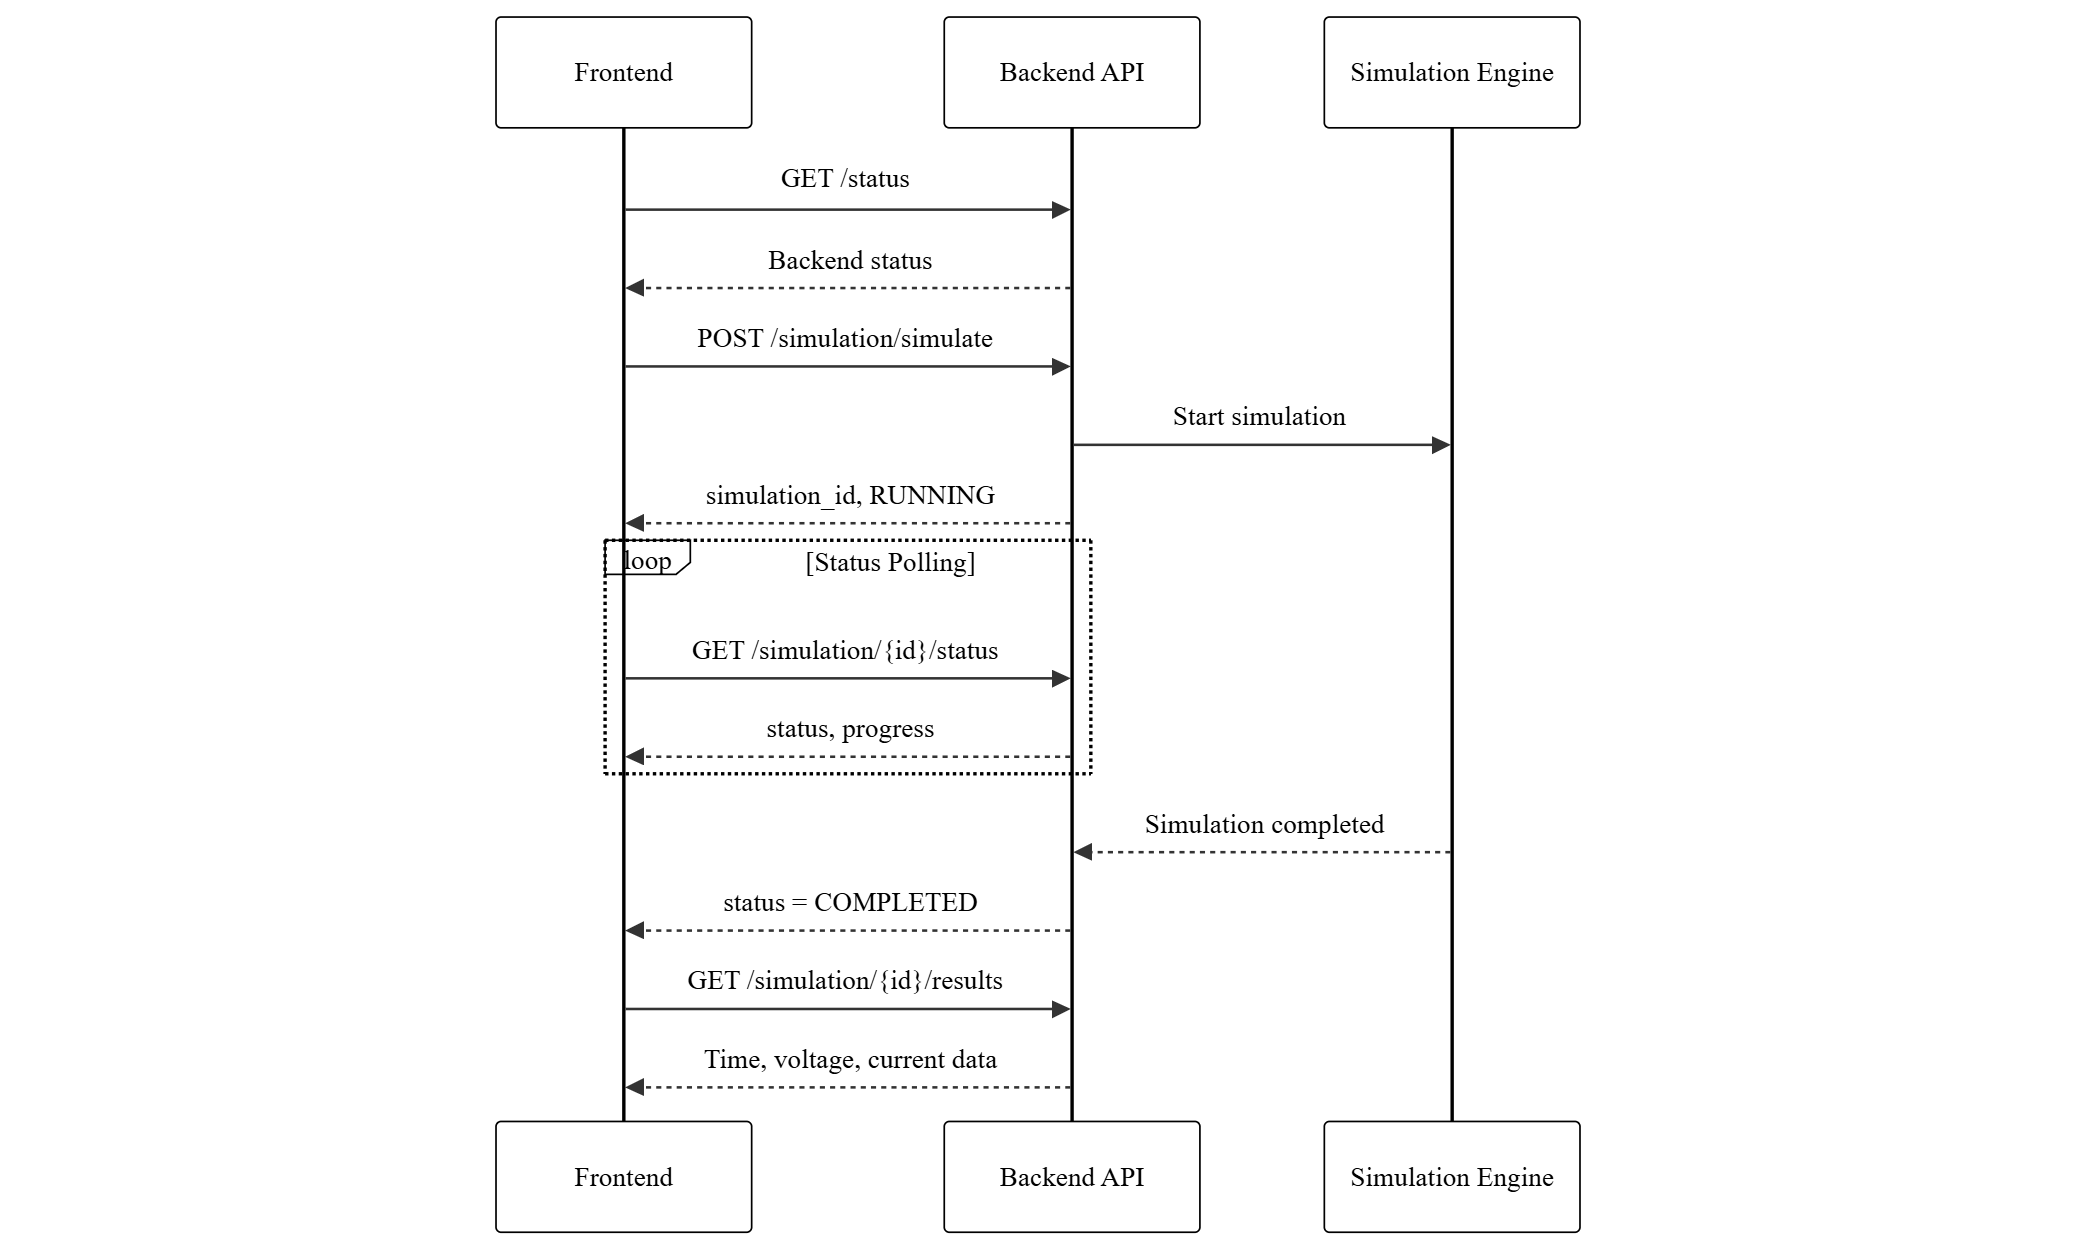
\includegraphics[width=\textwidth]{src/images/figures/backend_req_res.png}    \caption{Interaction Diagram for the Web Application}
    \label{fig:webapp-interaction}
\end{figure}

The frontend communicates with the backend through \gls{http} requests to the documented endpoints. User inputs from the editable circuit schematic are converted into \gls{spice} netlists and submitted to the simulation endpoint. The frontend periodically polls the status endpoint to track simulation progress, and upon completion, retrieves and visualizes the results using Chart.js for graph generation and React components for interactive display.

\section{Circuit Simulation using PySpice}

\gls{pyspice} is a \gls{python} interface to \gls{ngspice} (an open-source simulation engine) that takes in the netlist of the circuit and returns the data required to visualize graphs related to the circuit. The \gls{pyspice} integration allows the backend to programmatically define circuits, run simulations, and extract result data in a structured format suitable for visualization and analysis.

\subsection{Netlist to Simulation Results Conversion}

The process of converting a circuit netlist to simulation results involves several key steps: parsing the netlist, initializing the simulation environment, configuring analysis parameters, executing the simulation, and extracting the resulting voltage and current data in a format compatible with the frontend visualization system.

\begin{algorithm}
\caption{\gls{rc} Circuit Transient Simulation and Data Export}
\label{algo:rc-transient-simulation}
\begin{algorithmic}
\Require Supply voltage $V_s$, resistance $R$, capacitance $C$, simulation step $\Delta t$, simulation duration $T$
\Ensure \gls{csv} file containing transient voltage response
\State Initialize \gls{spice} circuit named \textit{RC Charging Circuit}
\State Enable logging for simulation diagnostics
\State \textbf{Define circuit components}
\State Add \gls{dc} voltage source of magnitude $V_s$ between input node and ground
\State Connect resistor $R$ between input node and node $n1$
\State Connect capacitor $C$ between node $n1$ and ground
\State Initialize simulator with nominal temperature
\State Perform transient analysis with step size $\Delta t$ up to time $T$
\State Extract time vector from transient analysis
\State Extract voltage waveform at node $n1$
\State Create data table mapping time to voltage
\State Export data table to \gls{csv} file
\State \Return Generated \gls{csv} file
\end{algorithmic}
\end{algorithm}


\chapter{RESULTS AND ANALYSIS}

%  WRITING GUIDELINES FOR RESULTS AND ANALYSIS CHAPTER
%  ====================================================
% The Results and Analysis chapter presents the outcomes of your project and critically analyzes
% them. This chapter demonstrates whether your system meets requirements, compares performance
% against objectives and baselines, and interprets findings. Results should be presented objectively
% with appropriate visualizations, while analysis provides context and explanation. This chapter should be full of charts, tables, and figures illustrating your system's performance and behaviour.


% %  LaTeX quick refs:
% \begin{itemize}
%     \item Always reference figures and tables in the text before they appear.
%     \item Use the cleveref package; write \verb|\cref{fig:label}| or \verb|\Cref{tab:label}| for automatic formatting (add \verb|\usepackage{cleveref}| to the preamble).
%     \item Keep captions descriptive and use unique labels per chapter (e.g., \texttt{fig:my-figure}, \texttt{tab:results}).
% \end{itemize}

\section{Comparative Analysis of Object Detection using YOLOv5 and YOLOv7}

\subsection{Experimental Setup}

A comparative study using \gls{yolo}v5 and \gls{yolo}v7 to detect and classify hand-drawn electronic circuit components was conducted to determine which model is better-suited for the needs of this project. The dataset consisted of 61 classes, including resistors, capacitors (polarized and unpolarized), diodes, transistors (\gls{bjt} and \gls{fet}), integrated circuits, switches, and more. To ensure a fair comparison, both models were trained and validated on identical data splits.

\subsection{Training Progress and Loss Curves}

While training, loss metrics (bounding box loss, objectness loss, and the classification loss) were tracked. The training curves show how these metrics evolved over time. No substantial difference was seen between the loss metrics of \gls{yolo}v5 and v7.

\begin{figure}[H]
    \centering
    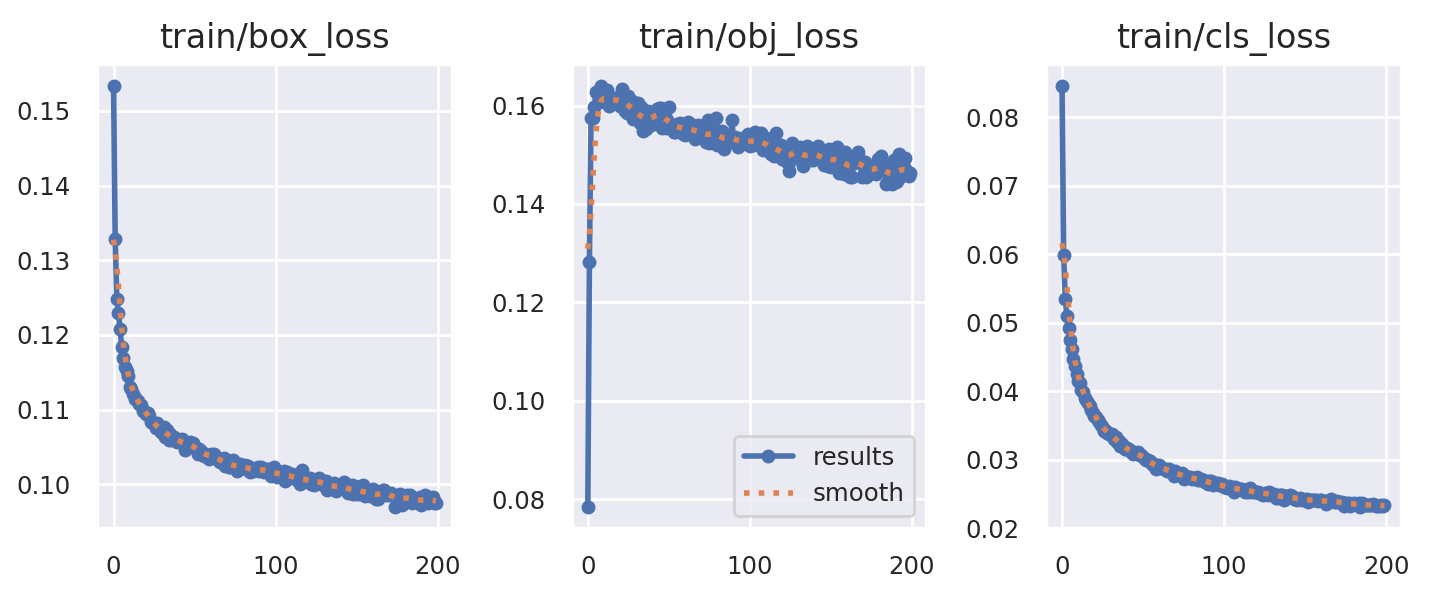
\includegraphics[width=\textwidth]{src/images/figures/loss_curve_yolov5.png}
    \caption{Loss Curves for YOLOv5}
    \label{fig:yolov5-loss-curves}
\end{figure}

\begin{figure}[H]
    \centering
    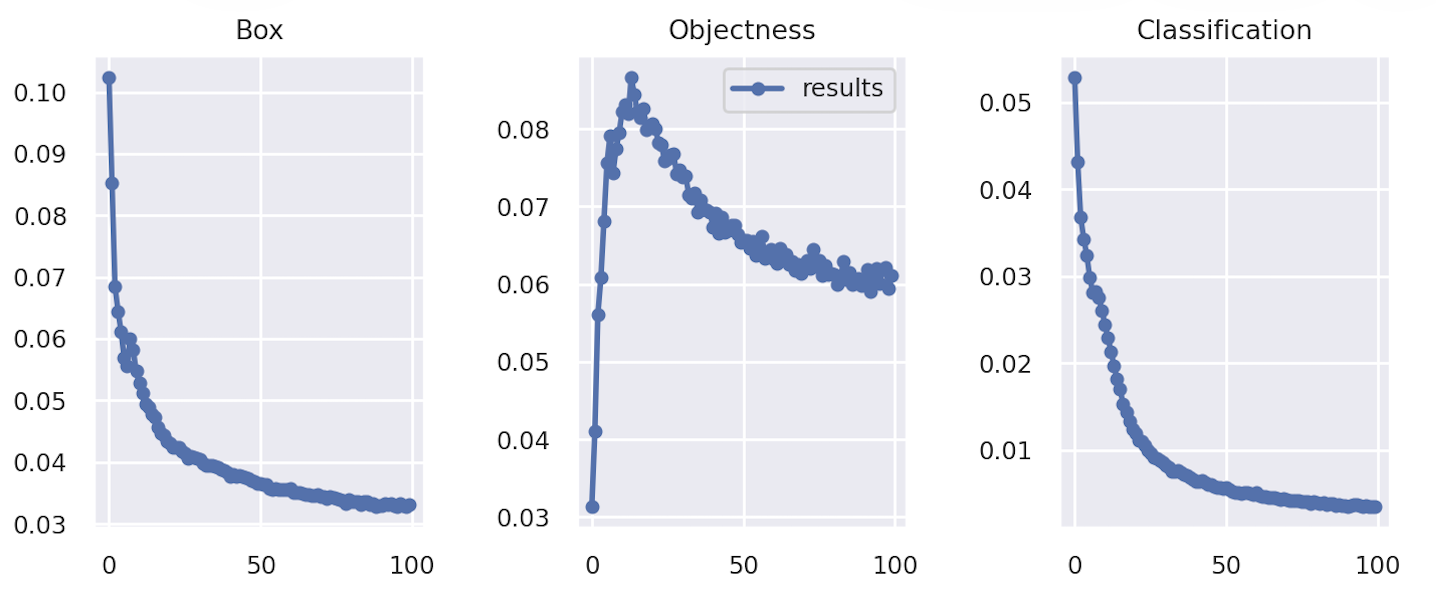
\includegraphics[width=\textwidth]{src/images/figures/loss_curve_yolov7.png}
    \caption{Loss Curves for YOLOv7}
    \label{fig:yolov7-loss-curves}
\end{figure}

\subsection{Performance Metrics}

\subsubsection{mAP vs Number of Epochs}

In order to monitor the progress in models' ability to recognize components as the training progressed, both \gls{map}@0.5 and \gls{map}@0.5:0.95 were plotted across all epochs. These curves depict how quickly and effectively each model learns over time.

\begin{figure}[H]
    \centering
    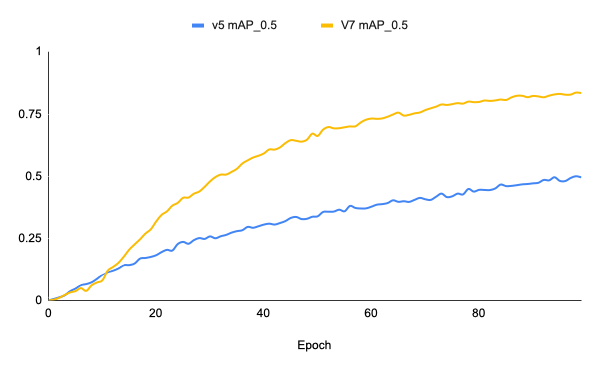
\includegraphics[width=\textwidth]{src/images/figures/map_vs_epochs.png}
    \caption{\gls{map}@0.5 vs Epochs for YOLOv5 and YOLOv7}
    \label{fig:map50-epochs}
\end{figure}

\begin{figure}[H]
    \centering
    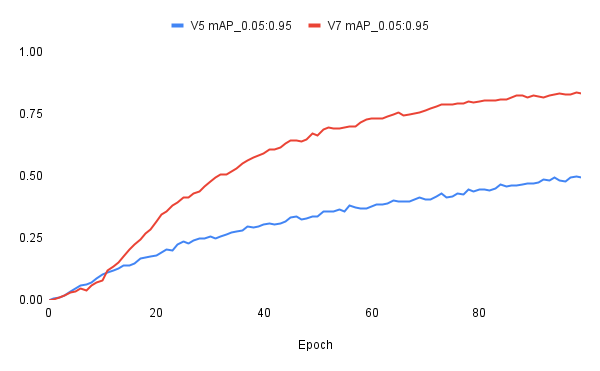
\includegraphics[width=\textwidth]{src/images/figures/map_vs_epochs_0.5to0.95.png}
    \caption{\gls{map}@0.5:0.95 vs Epochs for YOLOv5 and YOLOv7}
    \label{fig:map50-95-epochs}
\end{figure}

It is clear from both \cref{fig:map50-epochs} and \cref{fig:map50-95-epochs} that the \gls{map} scores for \gls{yolo}v7 are significantly better than that for \gls{yolo}v5. Likewise, the loss curves, as shown in \cref{fig:yolov5-loss-curves,fig:yolov7-loss-curves}, demonstrate a steeper curve in the case of YOLOv7.

\subsubsection{Precision, Recall, and F1 Score vs Confidence}

The following graphs demonstrate the model performance under varying confidence thresholds:

\paragraph{Precision vs Confidence}

\begin{figure}[H]
    \centering
    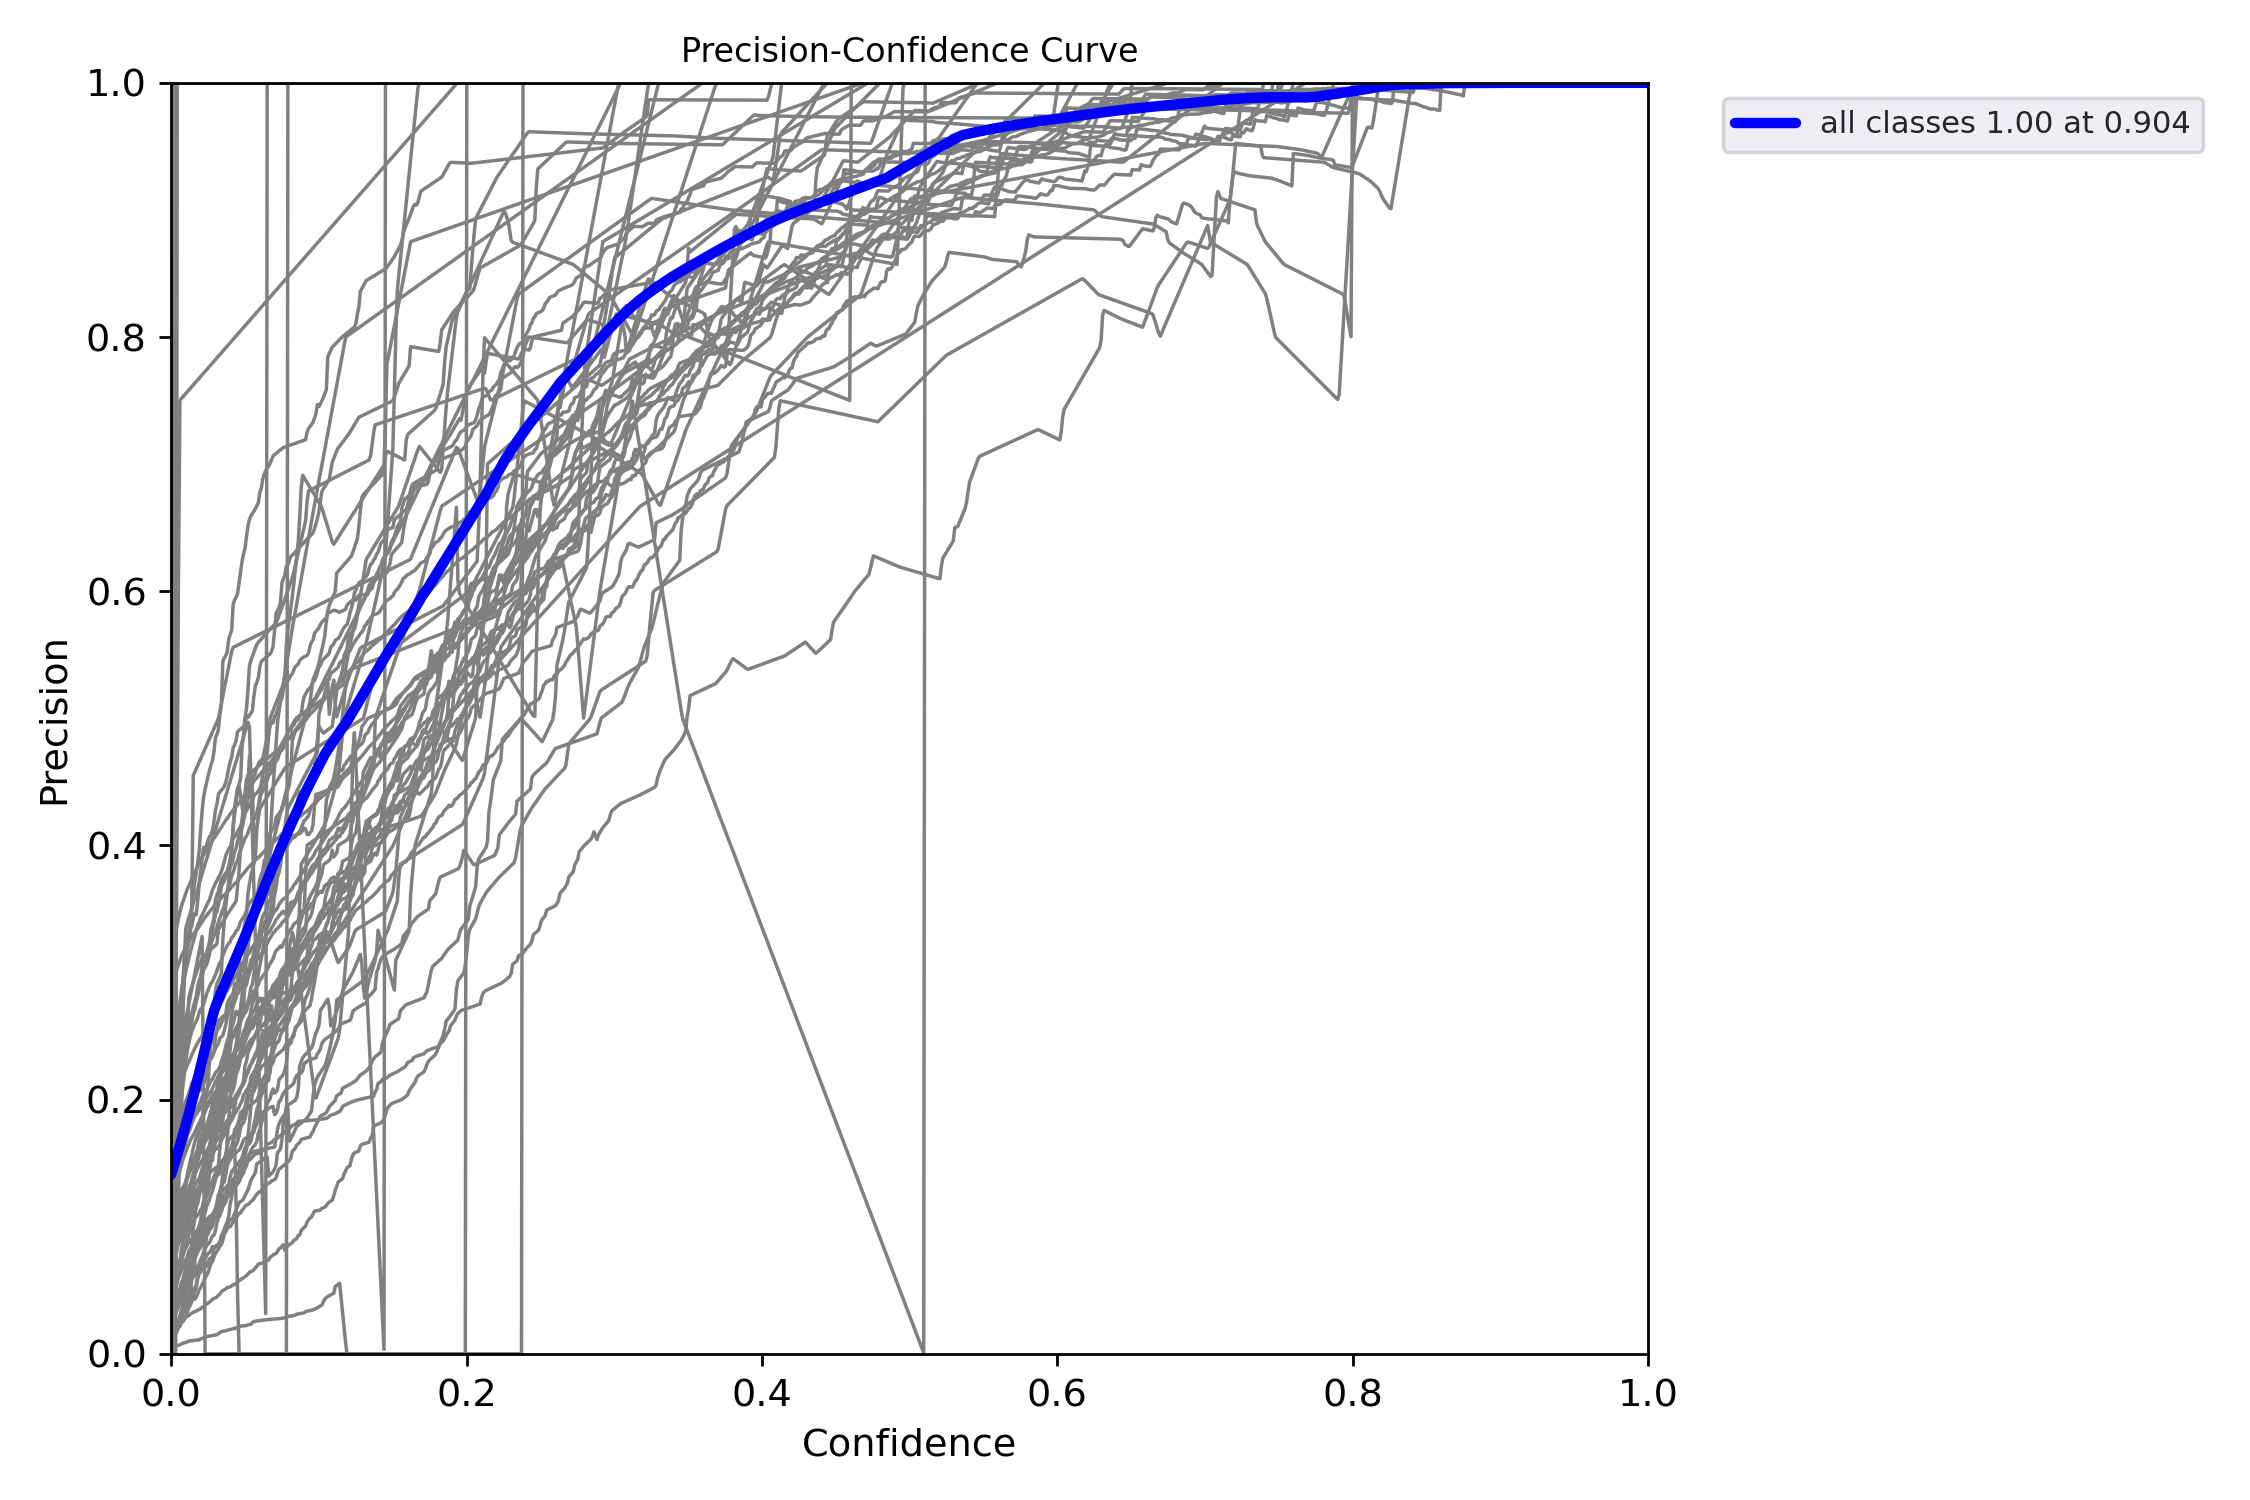
\includegraphics[width=\textwidth]{src/images/figures/precision_vs_confidence_yolov5.png}
    \caption{Precision-Confidence Curve for YOLOv5}
    \label{fig:precision-conf-v5}
\end{figure}

\begin{figure}[H]
    \centering
    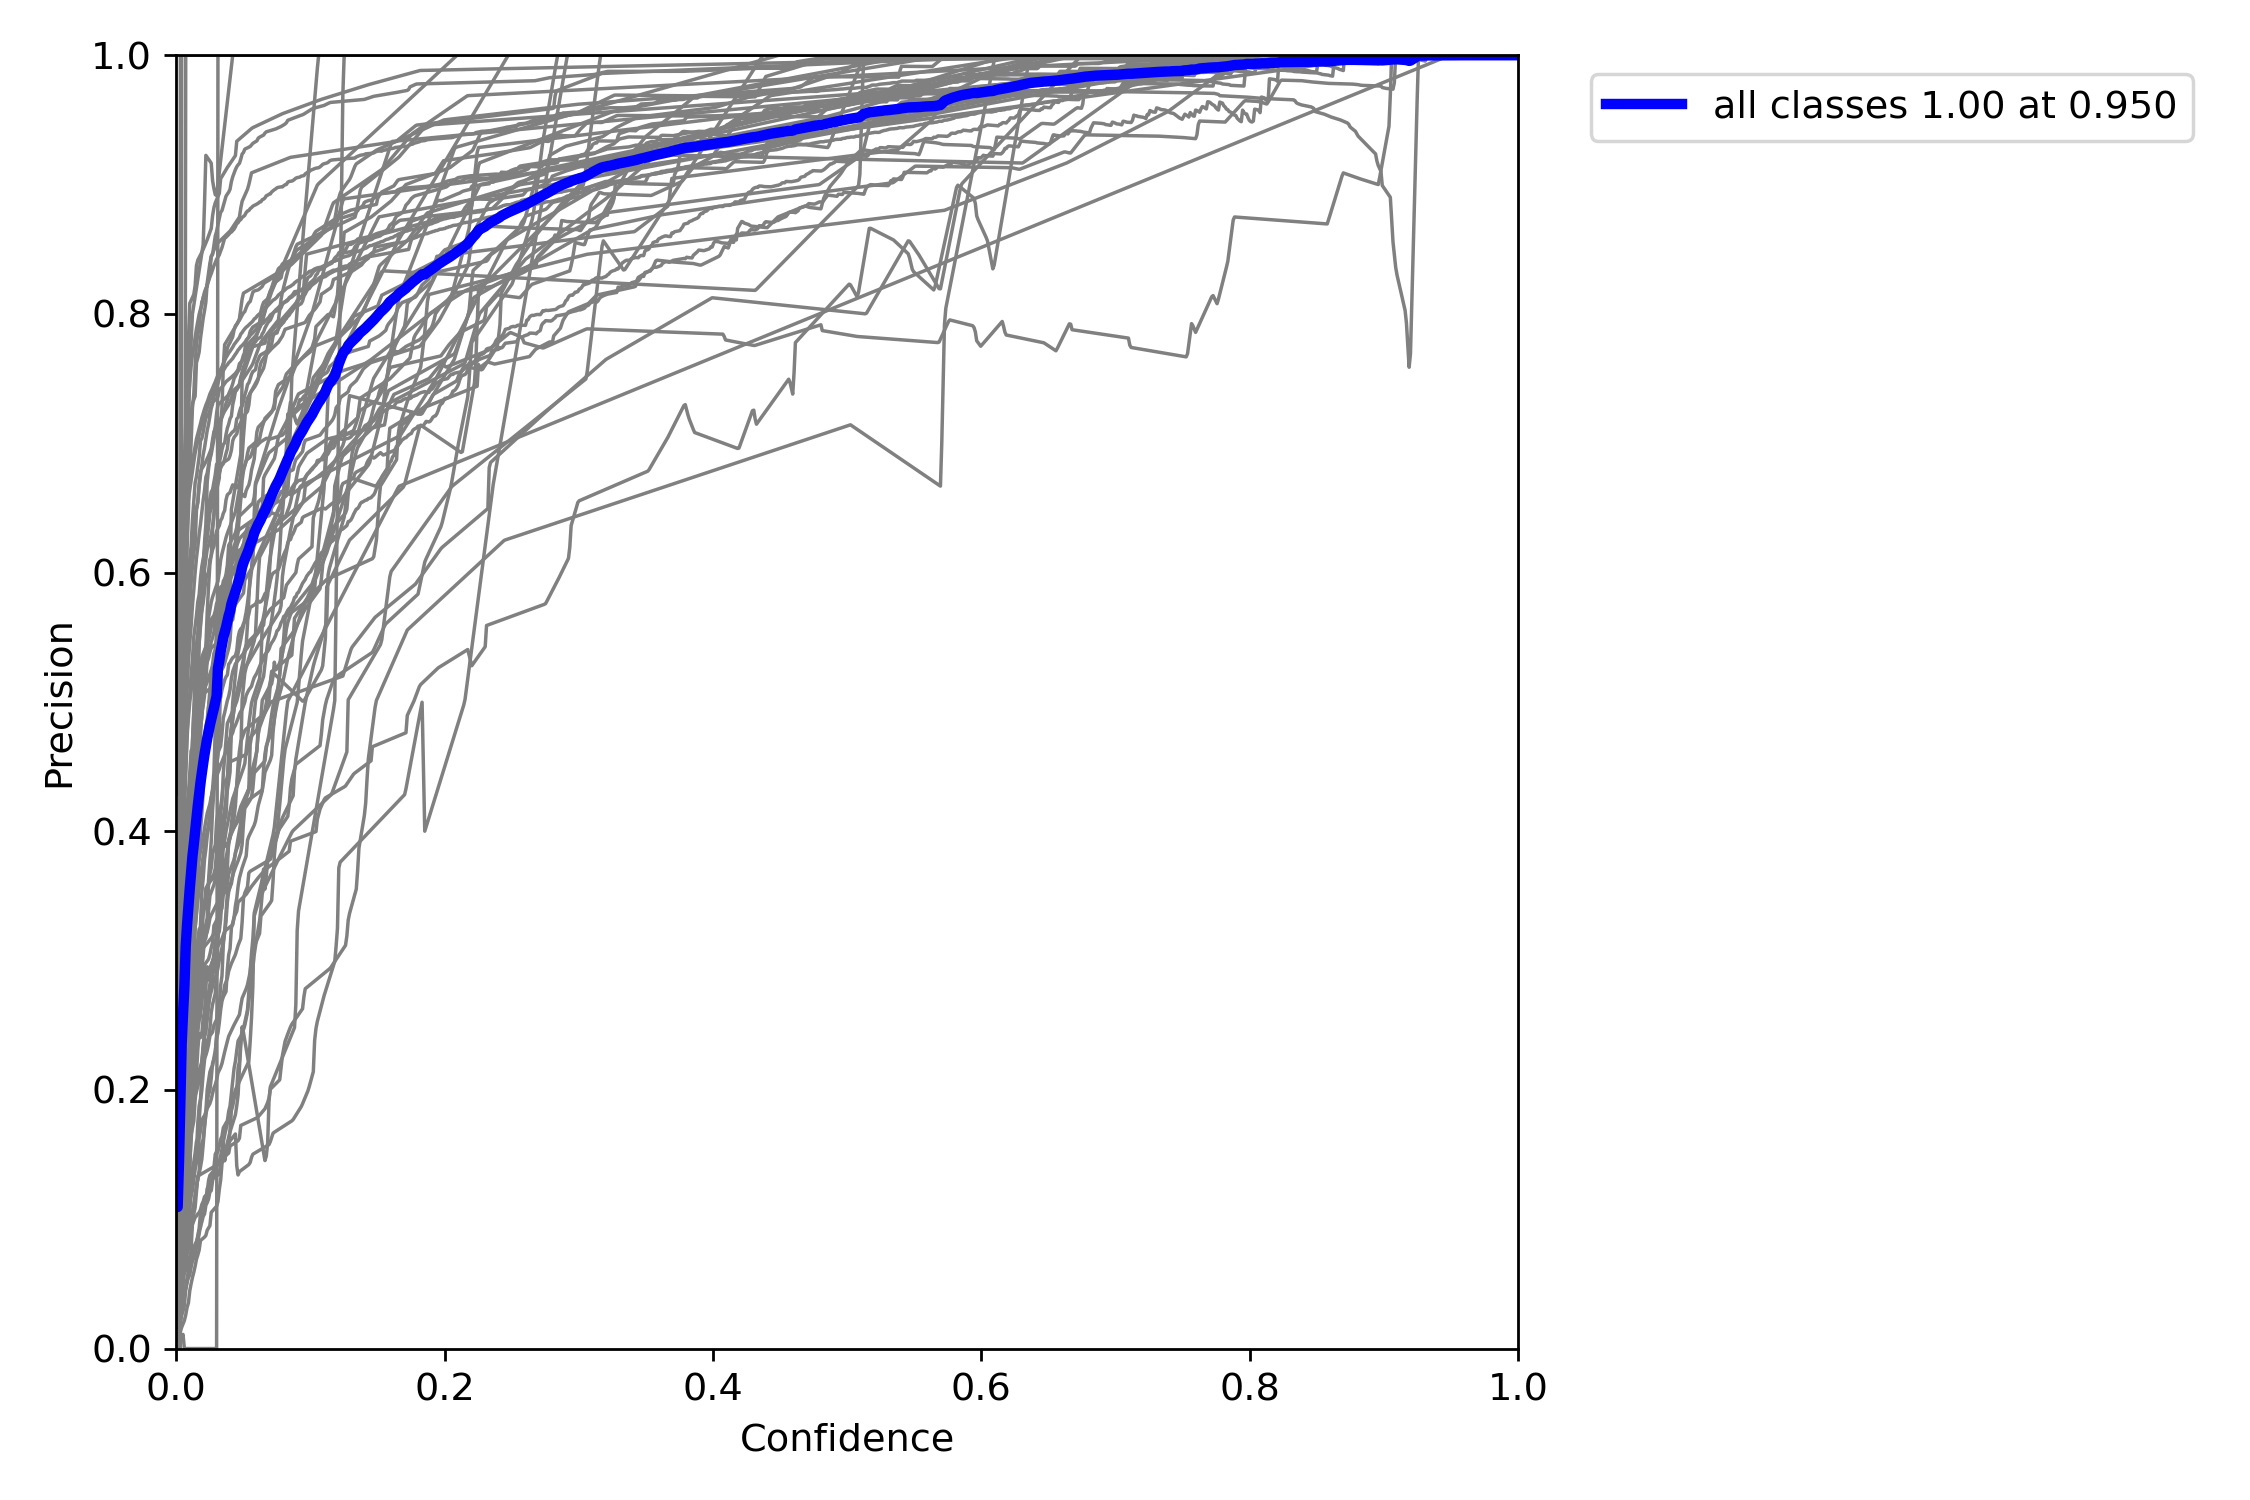
\includegraphics[width=\textwidth]{src/images/figures/precision_vs_confidence_yolov7.png}
    \caption{Precision-Confidence Curve for YOLOv7}
    \label{fig:precision-conf-v7}
\end{figure}

\cref{fig:precision-conf-v5} and \cref{fig:precision-conf-v7} demonstrate the Precision-Confidence Curve for YOLOv5 and YOLOv7 respectively. The area under this curve informs how consistently precise the model is across all confidence thresholds. For a large area under the curve, as in the case of YOLOv7, the model maintains good precision even when threshold changes; however, for a smaller area, precision collapses quickly when threshold is relaxed.

\paragraph{Recall vs Confidence}

\begin{figure}[H]
    \centering
    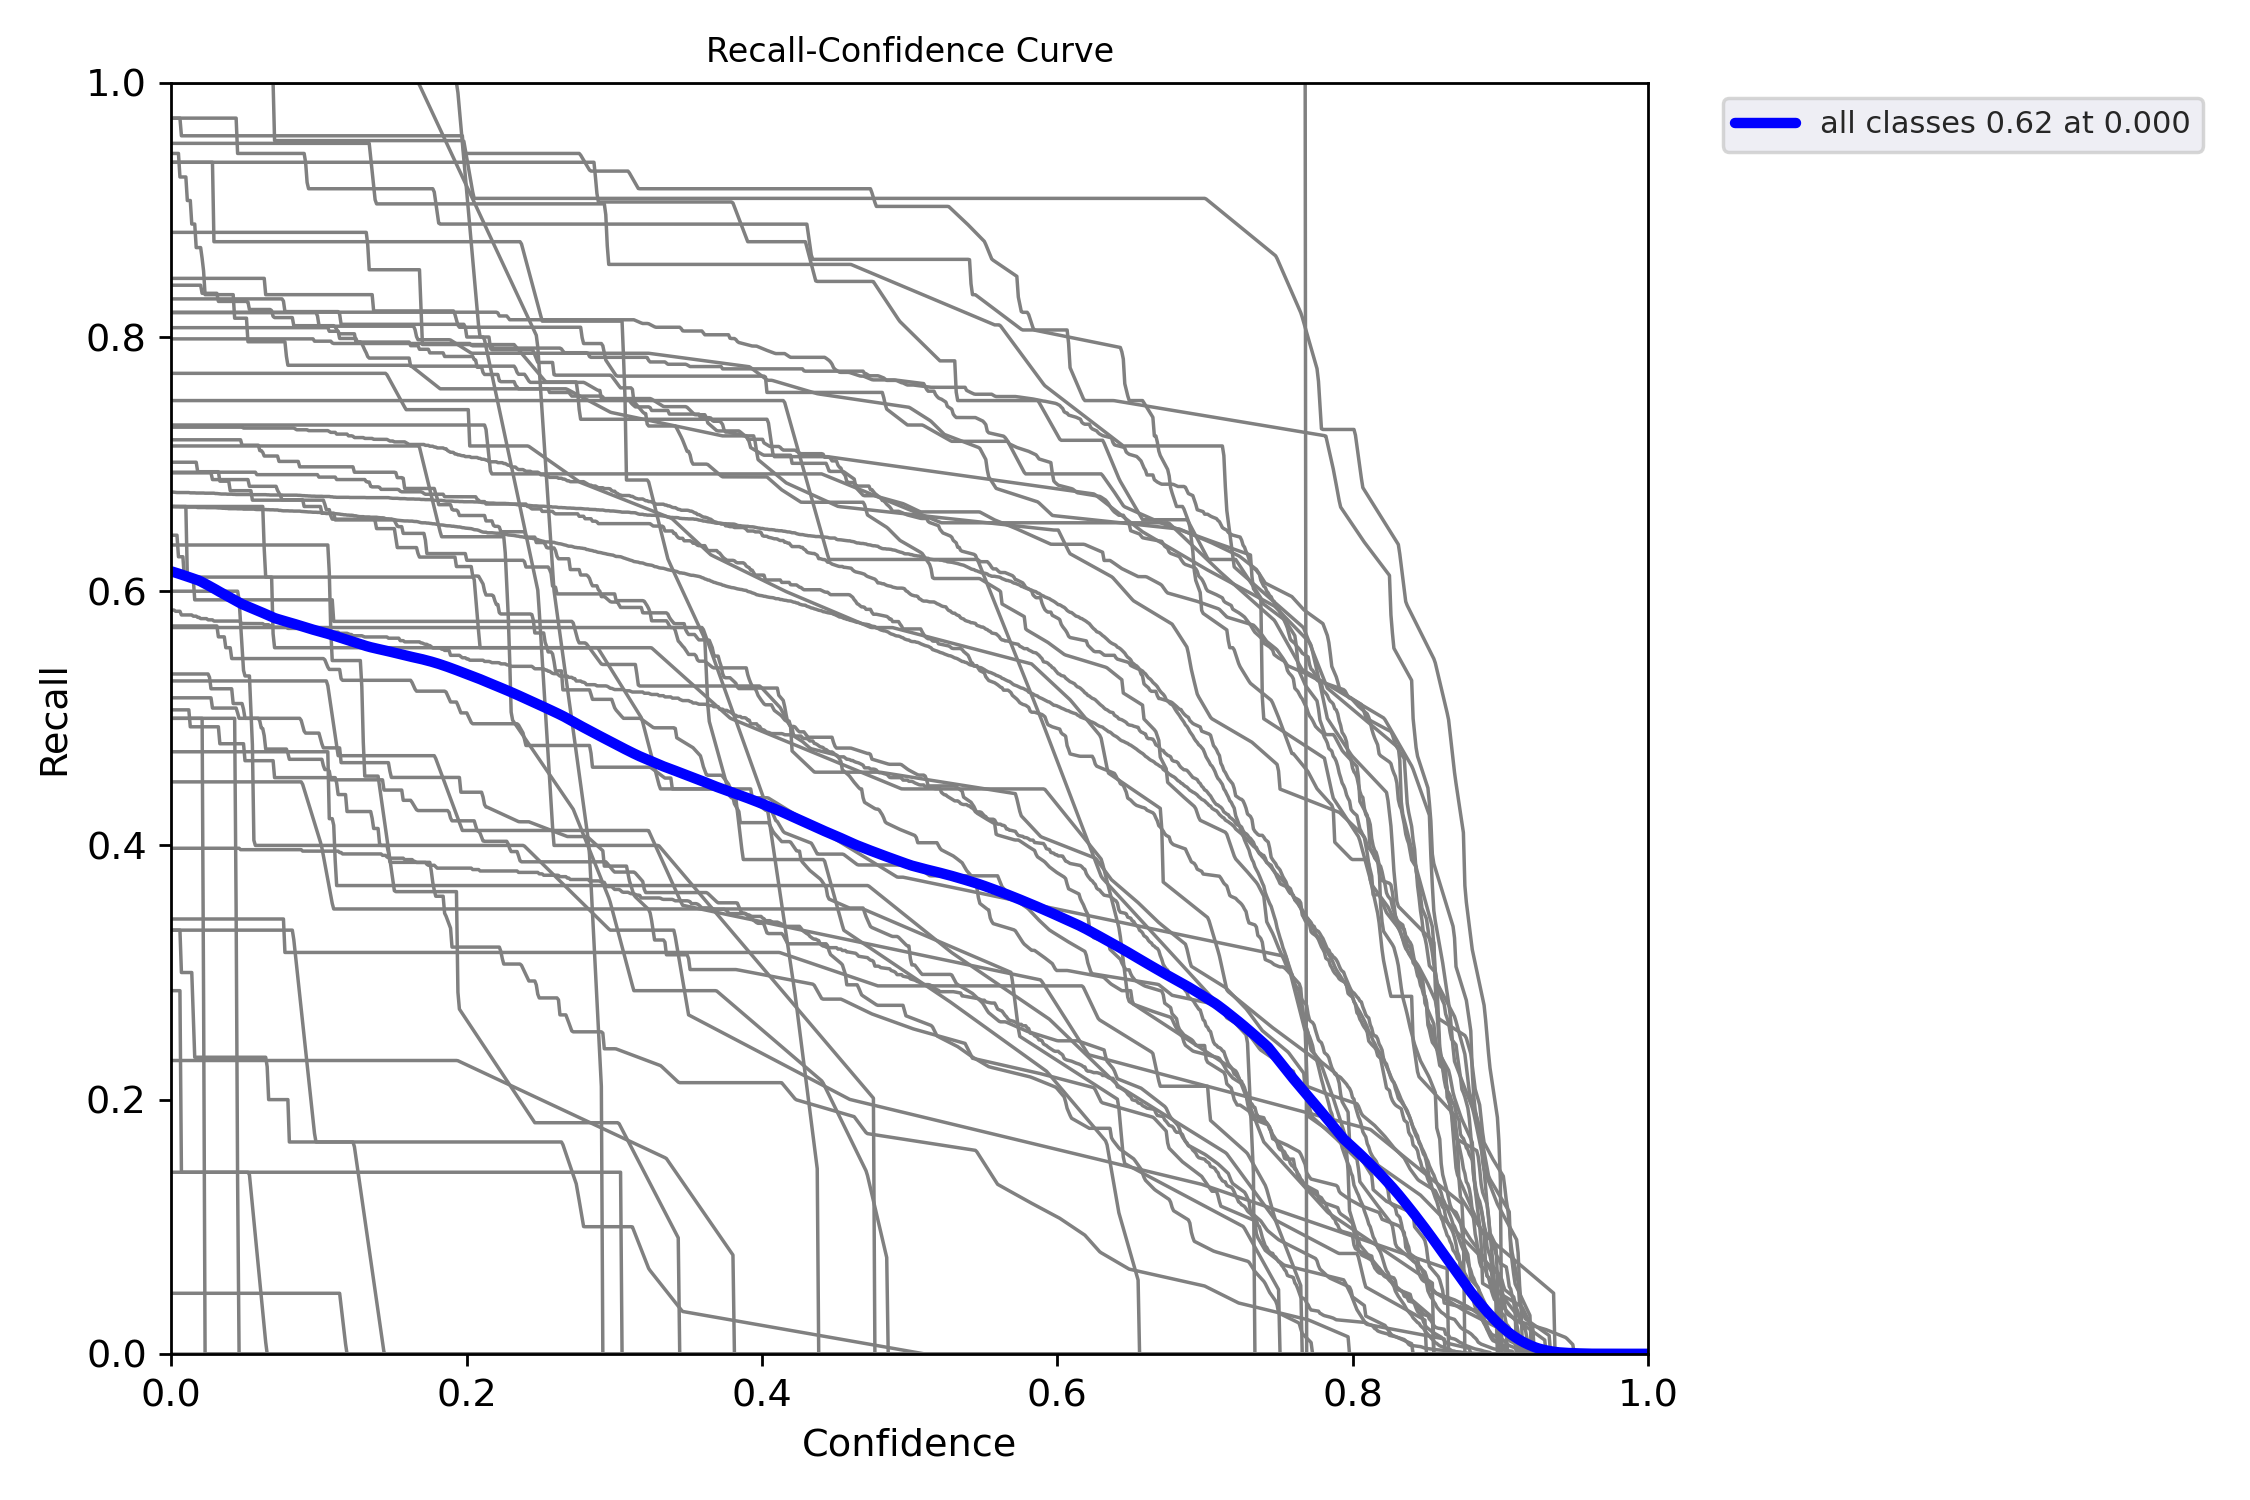
\includegraphics[width=\textwidth]{src/images/figures/recall_vs_confidence_yolov5.png}
    \caption{Recall-Confidence Curve for YOLOv5}
    \label{fig:recall-conf-v5}
\end{figure}

\begin{figure}[H]
    \centering
    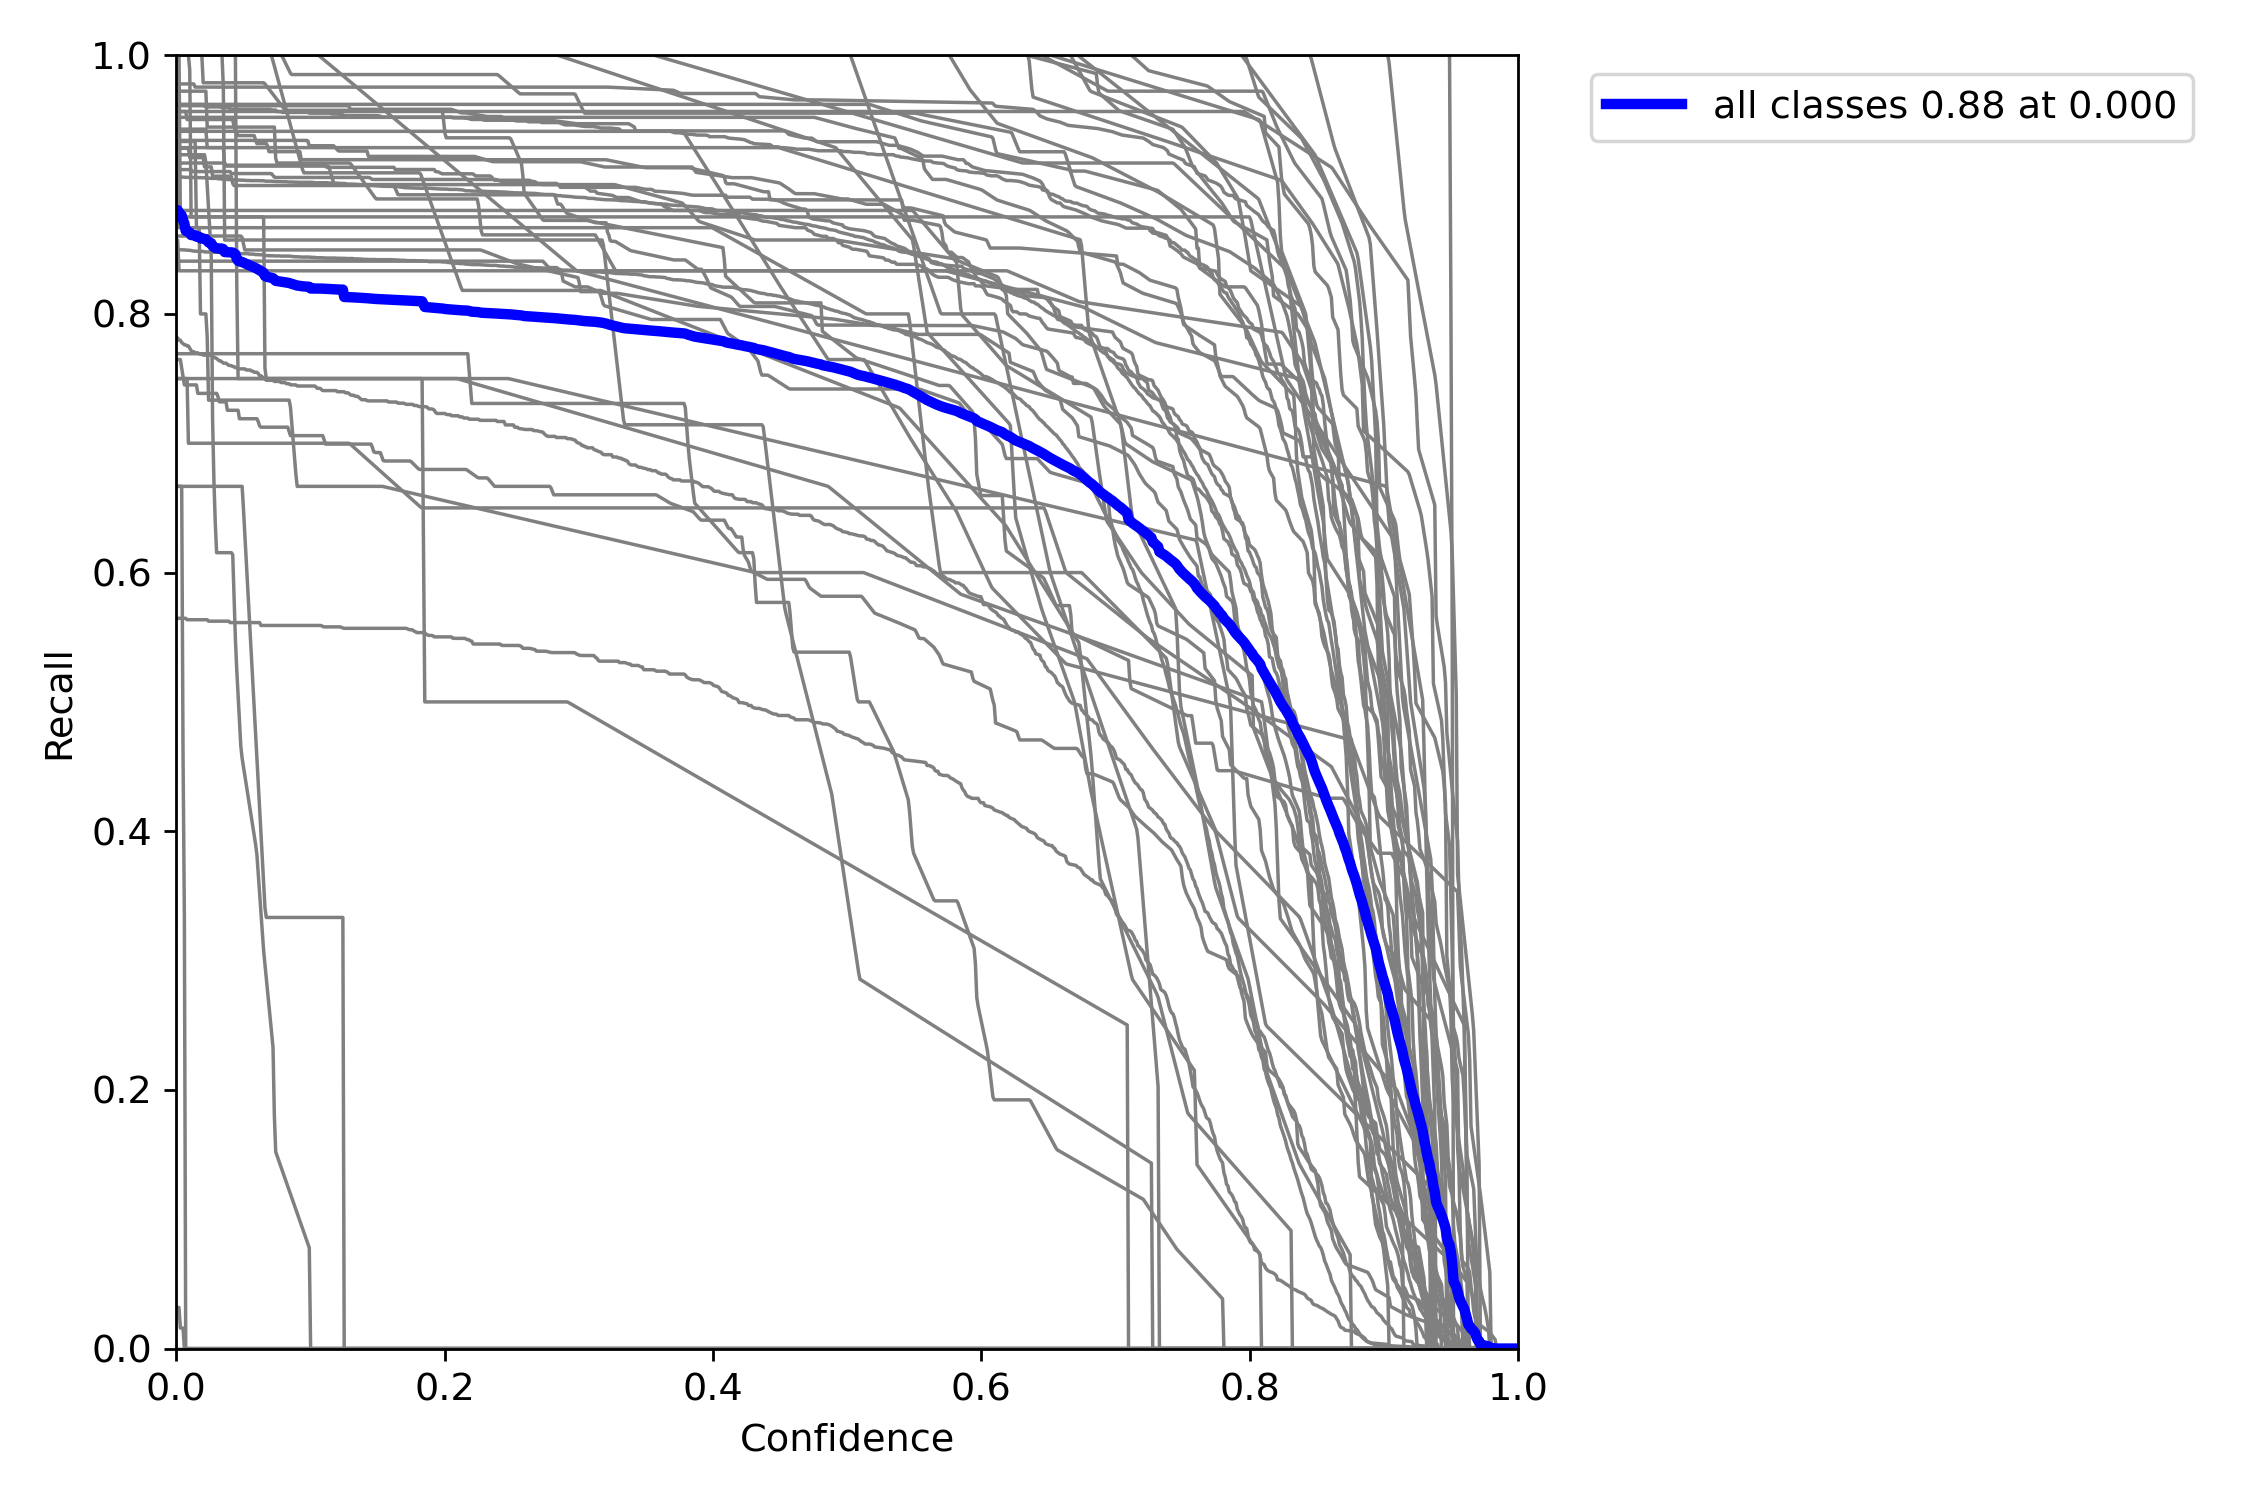
\includegraphics[width=\textwidth]{src/images/figures/recall_vs_confidence_yolov7.png}
    \caption{Recall-Confidence Curve for YOLOv7}
    \label{fig:recall-conf-v7}
\end{figure}

\cref{fig:recall-conf-v5} and \cref{fig:recall-conf-v7} demonstrate the Recall-Confidence Curve for YOLOv5 and YOLOv7 respectively. The area under this curve informs how well the model preserves recall while increasing certainty. For a large area, the recall stays high even with strict thresholds.

\paragraph{F1 Score vs Confidence}

\begin{figure}[H]
    \centering
    \includegraphics[width=\textwidth]{src/images/figures/f1_vs_confidence_yolov5.png}
    \caption{F1 Score-Confidence Curve for YOLOv5}
    \label{fig:f1-conf-v5}
\end{figure}

\begin{figure}[H]
    \centering
    \includegraphics[width=\textwidth]{src/images/figures/f1_vs_confidence_yolov7.png}
    \caption{F1 Score-Confidence Curve for YOLOv7}
    \label{fig:f1-conf-v7}
\end{figure}

\cref{fig:f1-conf-v5} and \cref{fig:f1-conf-v7} demonstrate the F1 Score-Confidence Curve for YOLOv5 and YOLOv7 respectively. The larger the area under this curve, the higher the robustness of the precision-recall trade-off across thresholds.

\paragraph{Precision-Recall Curve}

\begin{figure}[H]
    \centering
    \includegraphics[width=\textwidth]{src/images/figures/pr_curve_yolov5.png}
    \caption{Precision-Recall Curve for YOLOv5}
    \label{fig:pr-curve-v5}
\end{figure}

\begin{figure}[H]
    \centering
    \includegraphics[width=\textwidth]{src/images/figures/pr_curve_yolov7.png}    
    \caption{Precision-Recall Curve for YOLOv7}
    \label{fig:pr-curve-v7}
\end{figure}

\cref{fig:pr-curve-v5} and \cref{fig:pr-curve-v7} demonstrate the Precision-Recall Curve for YOLOv5 and YOLOv7 respectively. The area under this curve gives the average precision (AP) which informs how good the model is at ranking positive samples above negative ones. The area under each of the curves in these figures is higher for YOLOv7 in comparison to YOLOv5. This is expected behavior and proves YOLOv7 is better than YOLOv5 when it comes to performance. Although YOLOv7 is computationally more intensive and generally heavier than YOLOv5, this is a trade-off willing to be accepted to gain performance.

\subsection{Confusion Matrix}

To assess per-class performance, confusion matrices were generated using the validation set.

\begin{figure}[H]
    \centering
    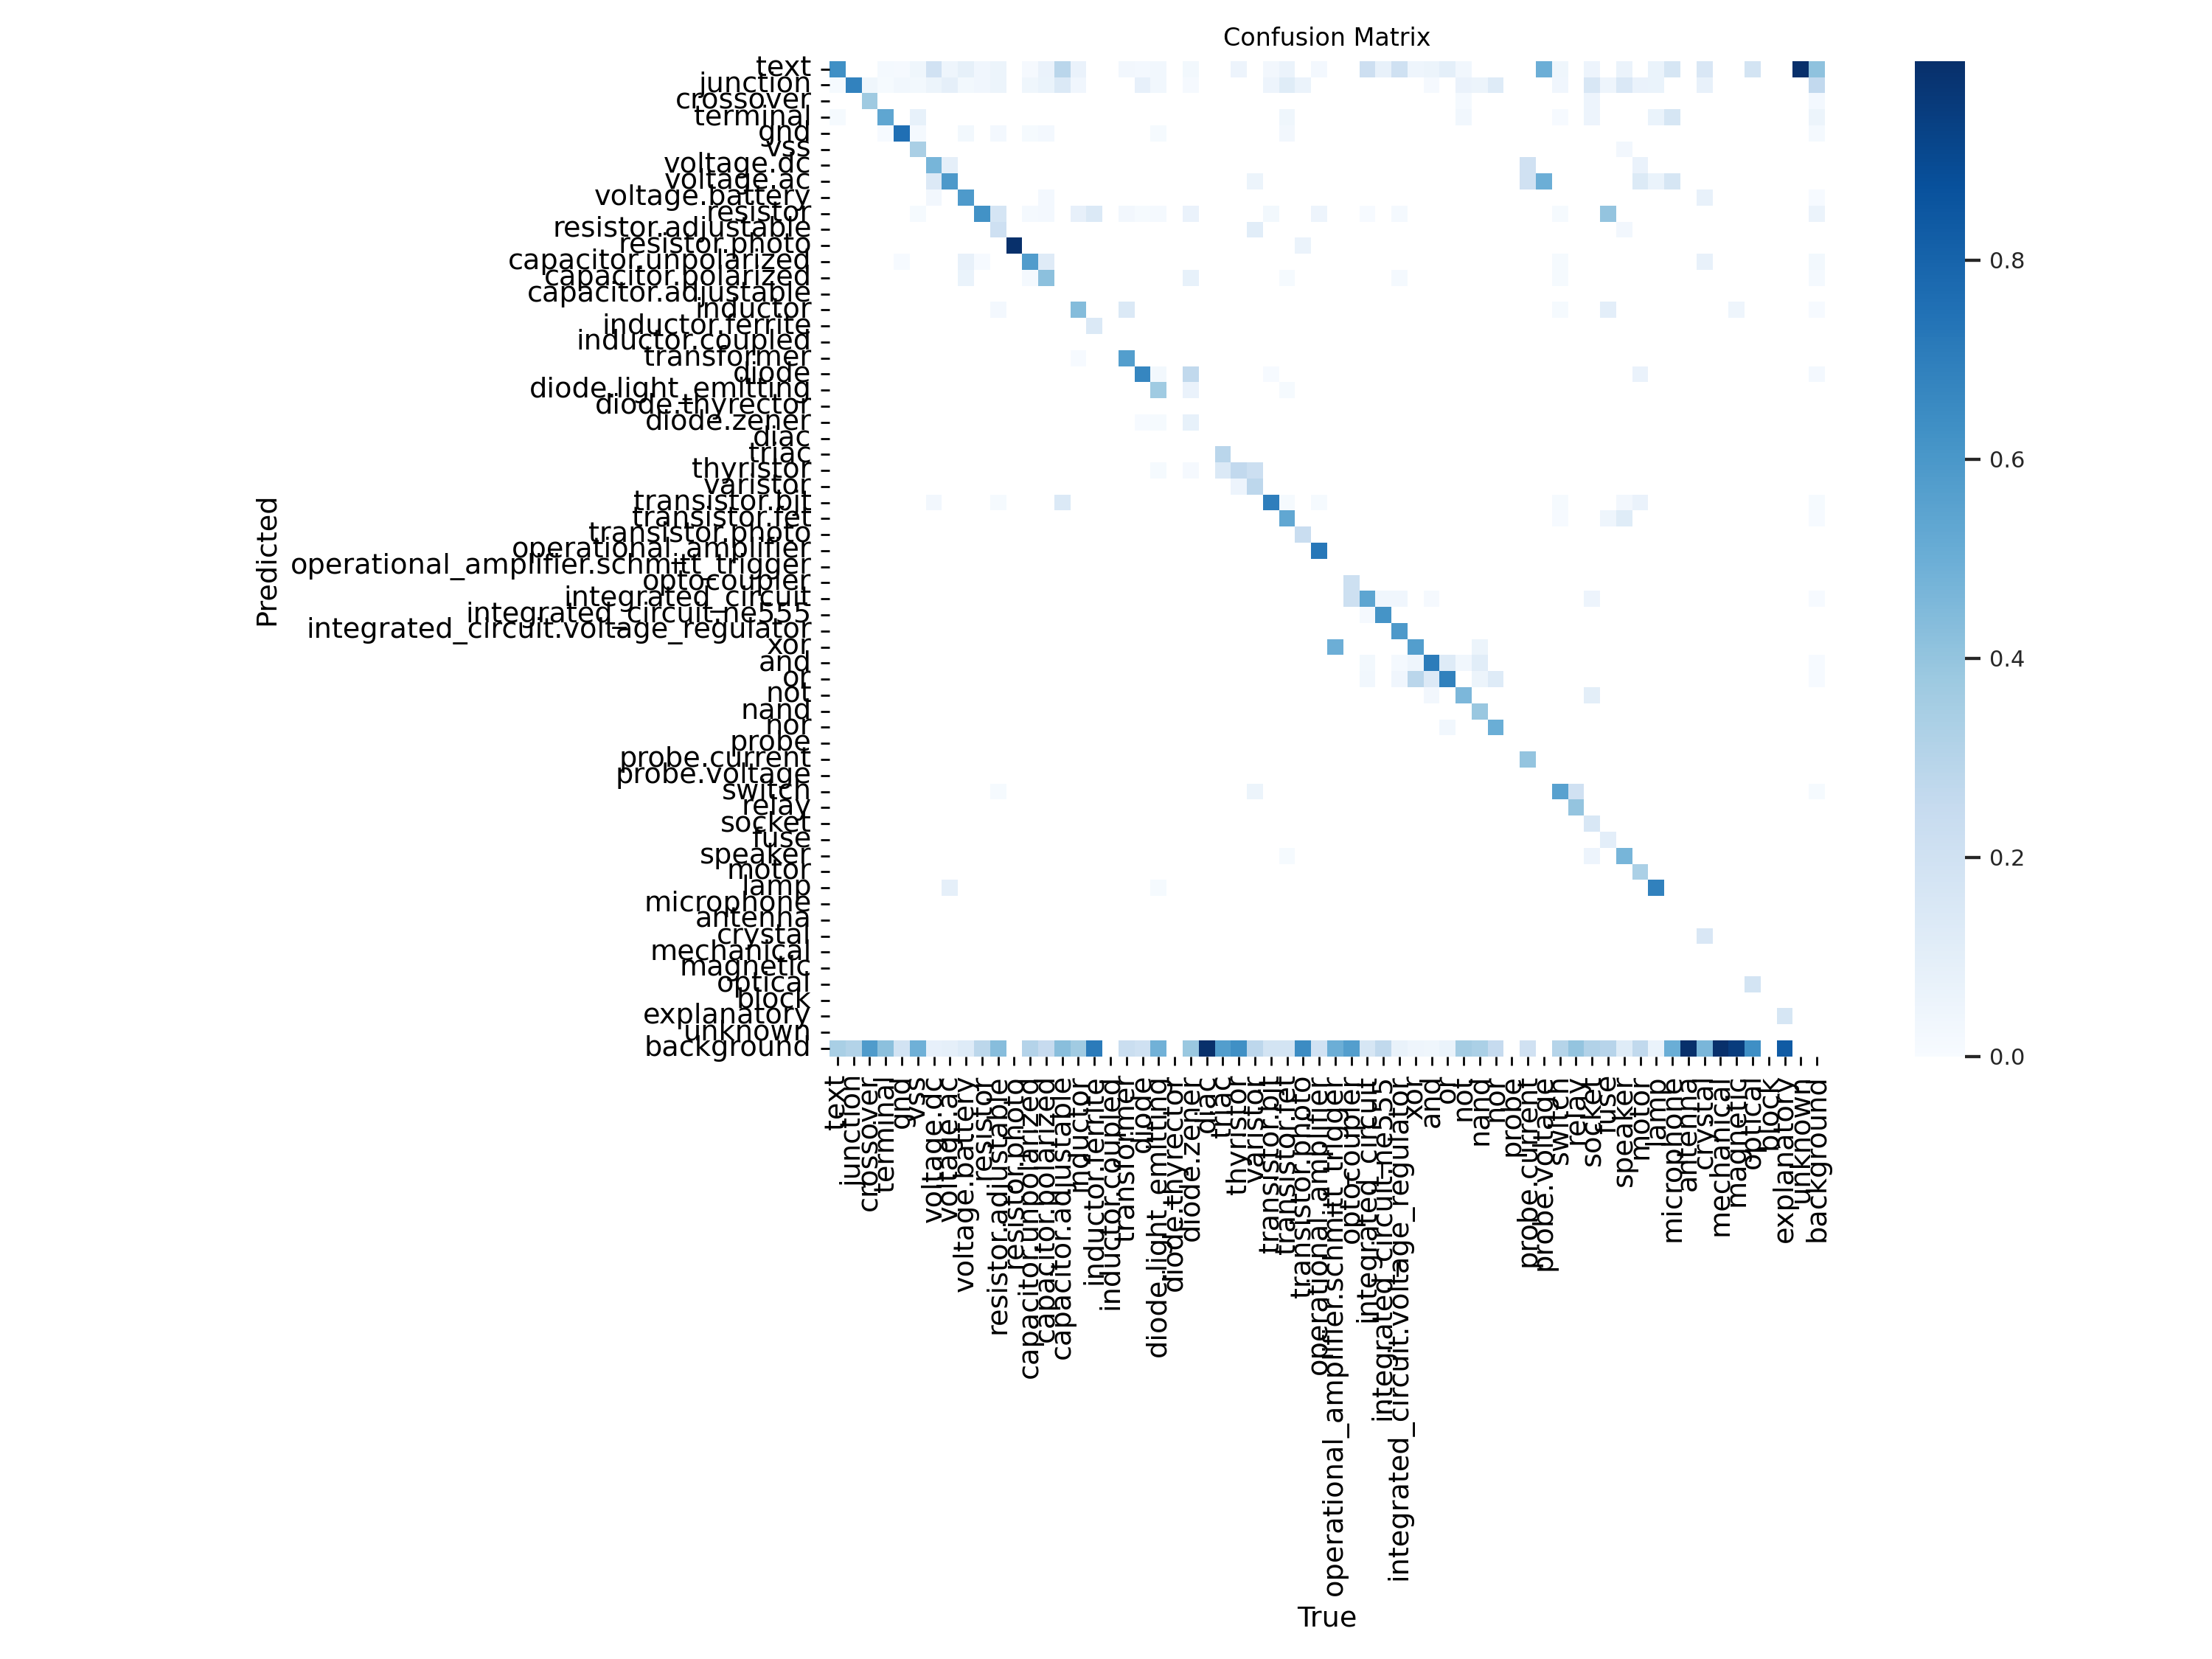
\includegraphics[width=\textwidth]{src/images/figures/confusion_matrix_yolov5.png}
    \caption{Confusion Matrix for YOLOv5}
    \label{fig:confusion-matrix-v5}
\end{figure}

\begin{figure}[H]
    \centering
    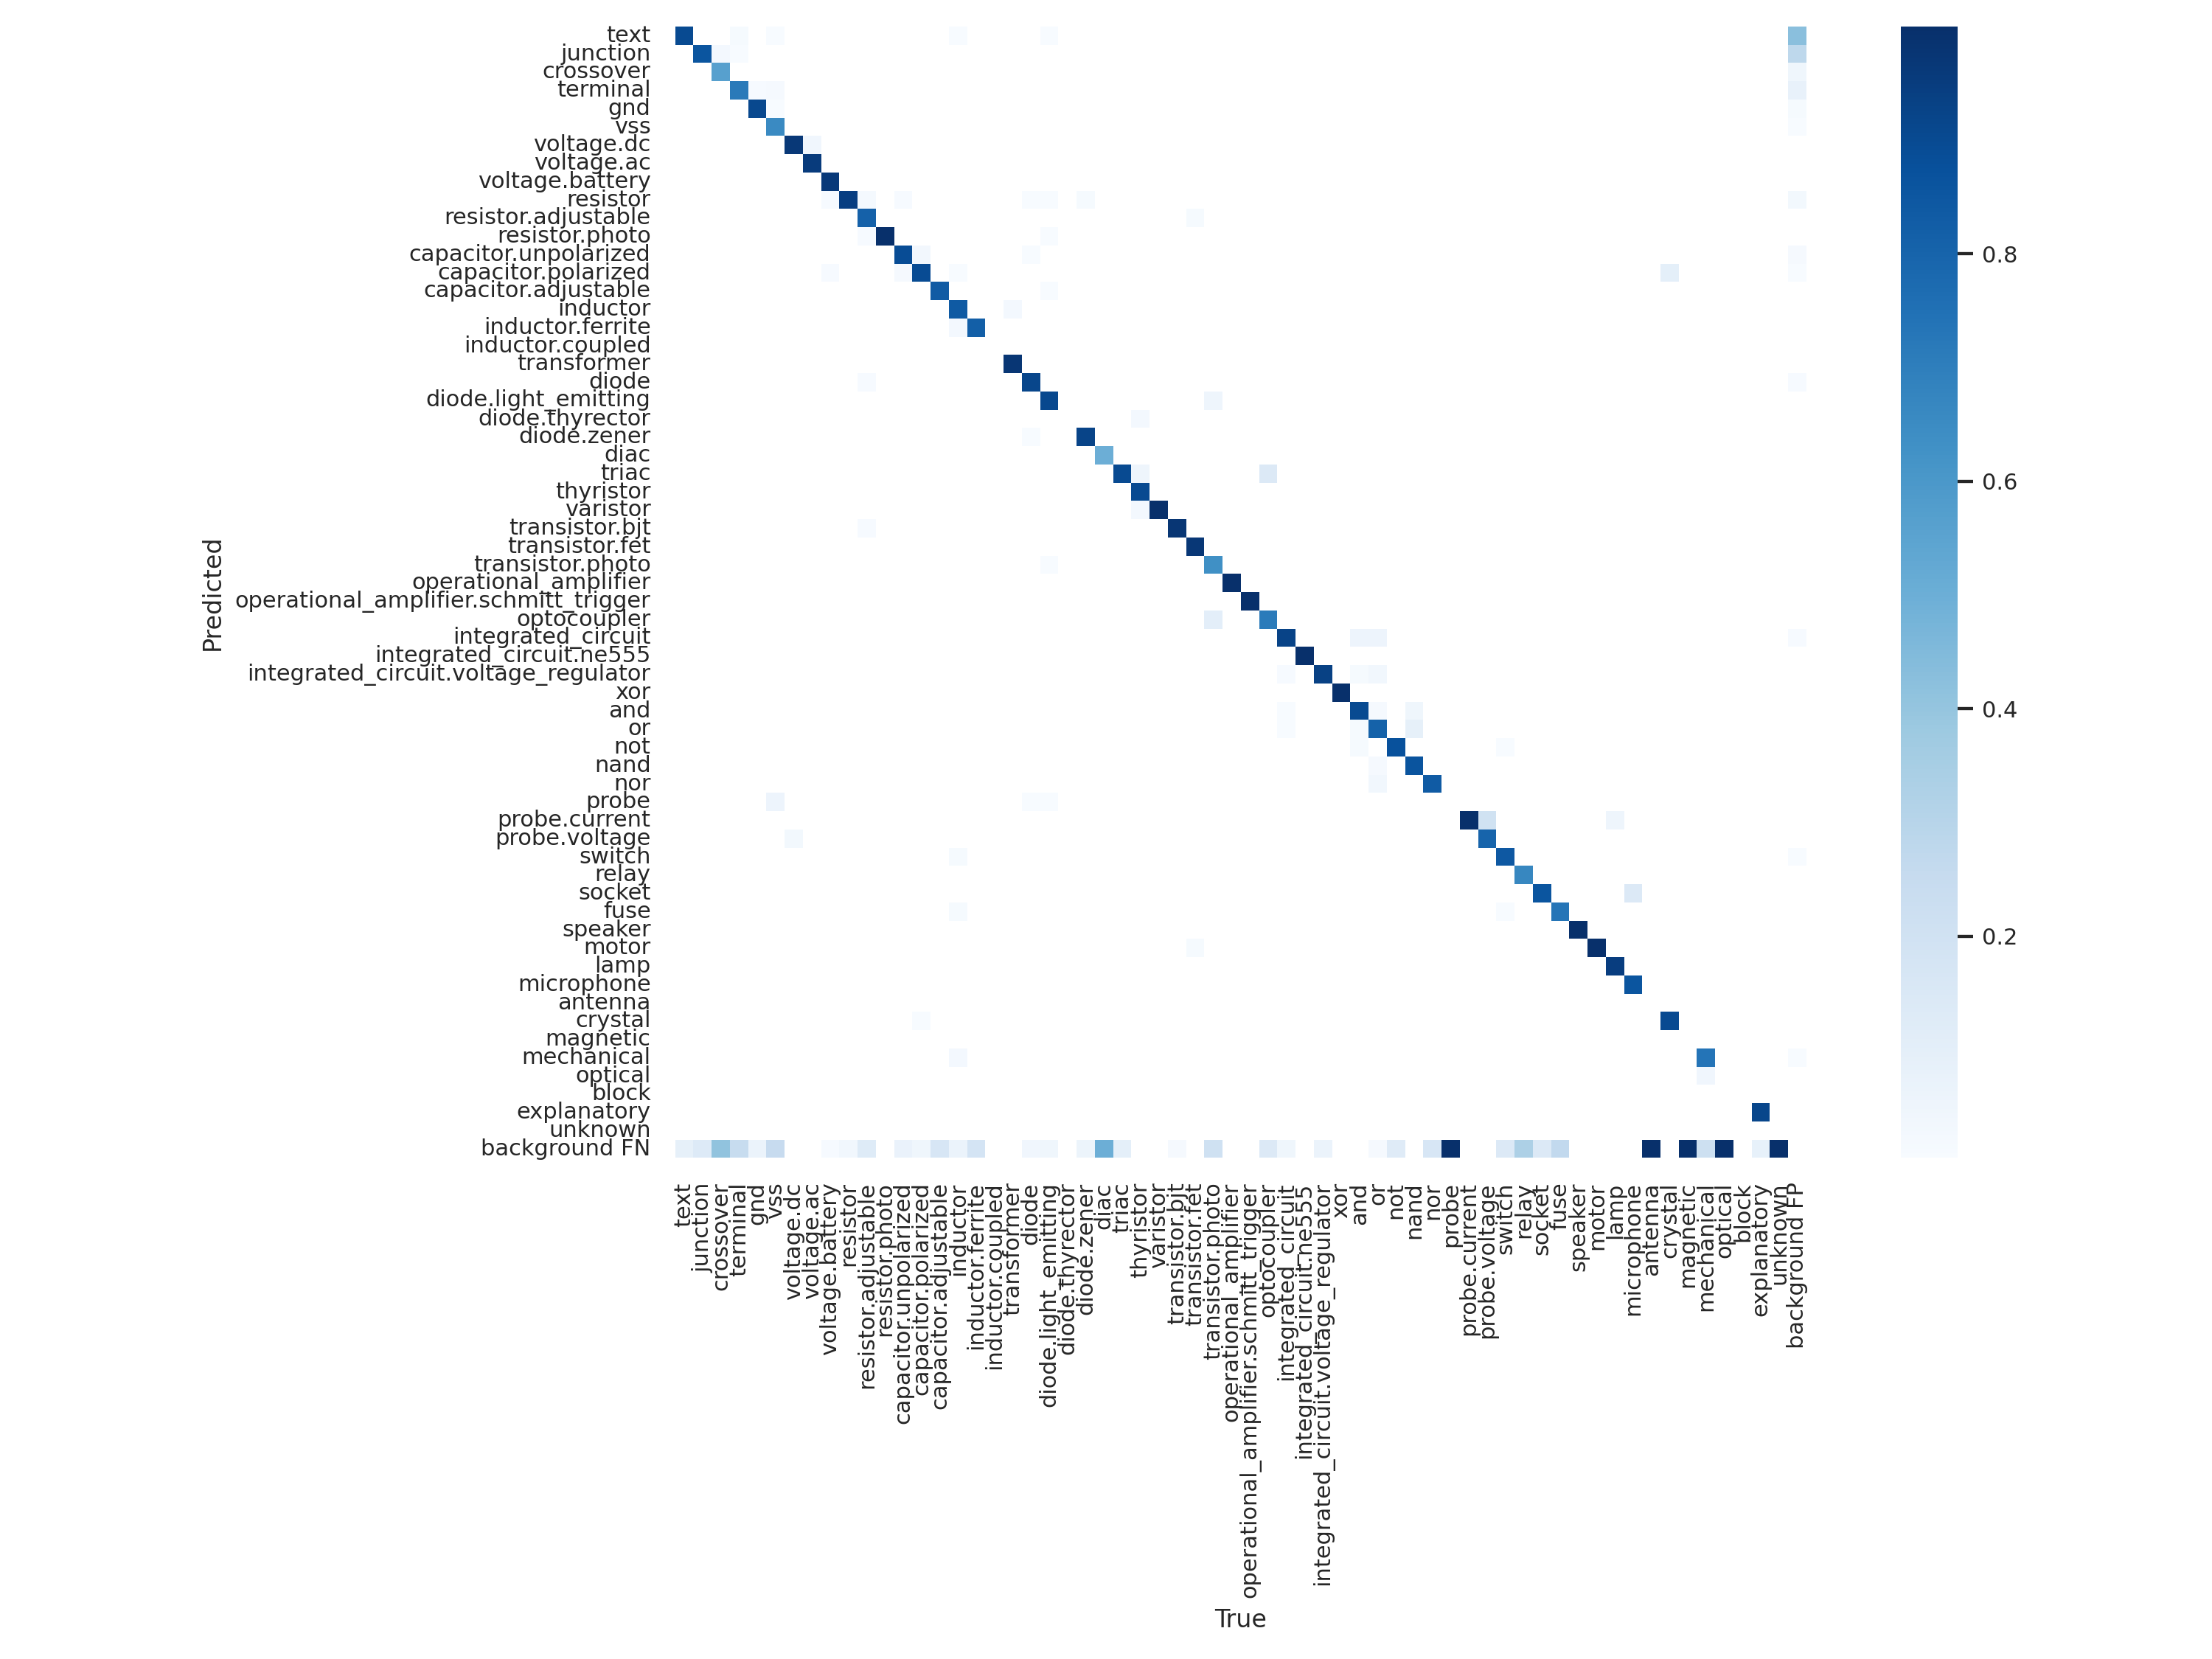
\includegraphics[width=\textwidth]{src/images/figures/confusion_matrix_yolov7.png}    
    \caption{Confusion Matrix for YOLOv7}
    \label{fig:confusion-matrix-v7}
\end{figure}

\cref{fig:confusion-matrix-v5} and \cref{fig:confusion-matrix-v7} demonstrate the confusion matrices for YOLOv5 and YOLOv7 respectively. In comparison, the confusion matrix for YOLOv7 has a very dark main diagonal and very light off-diagonals, which means that the model exhibits strong class separability with minimal inter-class confusion.

\subsection{Quantitative Results Comparison}

Final epoch results show \gls{yolo}v7 outperformed \gls{yolo}v5 across all major metrics.

\begin{table}[H]
    \centering
    \caption{Comparison of Performance Metrics for YOLOv5 and YOLOv7}
    \label{table:yolo-comparison}
    \begin{tabular}{lrr}
        \toprule
        \textbf{Metric} & \textbf{YOLOv5} & \textbf{YOLOv7} \\
        \midrule
        \gls{map}@0.5 & 0.61 & 0.83 \\
        \gls{map}@0.5:0.95 & 0.41 & 0.60 \\
        Precision & 0.84 & 0.93 \\
        Recall & 0.62 & 0.78 \\
        Epochs Trained & 200 & 100 \\
        \bottomrule
    \end{tabular}
\end{table}

Overall, \gls{yolo}v7 showed a clear advantage over \gls{yolo}v5 in our experiments. It not only achieved higher values for precision, recall, and mean average precision but also required fewer epochs to converge. \gls{yolo}v7's confusion matrix reflected better class separation and fewer misclassifications. The improvements in F1 score and overall stability of predictions across confidence thresholds make \gls{yolo}v7 a more robust choice for circuit diagram interpretation.

\section{\gls{ocr} Results}

The out-of-the-box default \gls{easyocr} implementation without fine-tuning was able to detect some of the component values from the circuit; however, the results left a lot to be desired. This made it clear that proper training of the recognition model is absolutely essential for this project.

After training the text recognition model from scratch, results were much improved. Two randomly picked images from the dataset are shown below after passing through the detection (\gls{yolo}v7) and recognition (\gls{ocr}) models.

\begin{figure}[H]
    \centering
    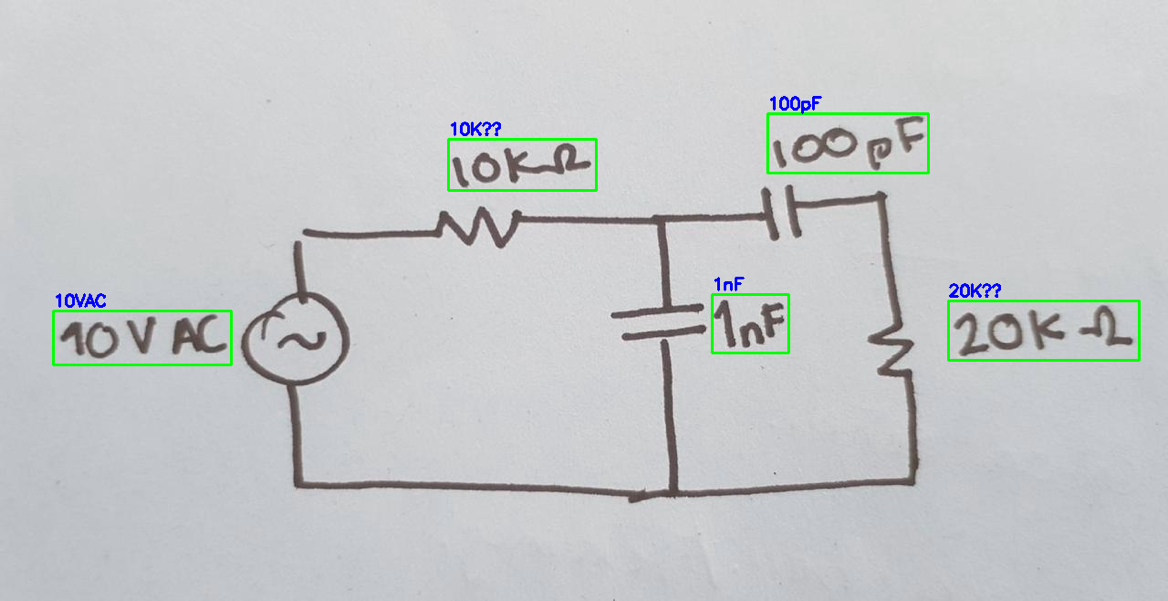
\includegraphics[width=\textwidth]{src/images/figures/text_detection_recognition.png}
    \caption{Text Detection and Recognition (i)}
    \label{fig:ocr-result-1}
\end{figure}

\begin{figure}[H]
    \centering
    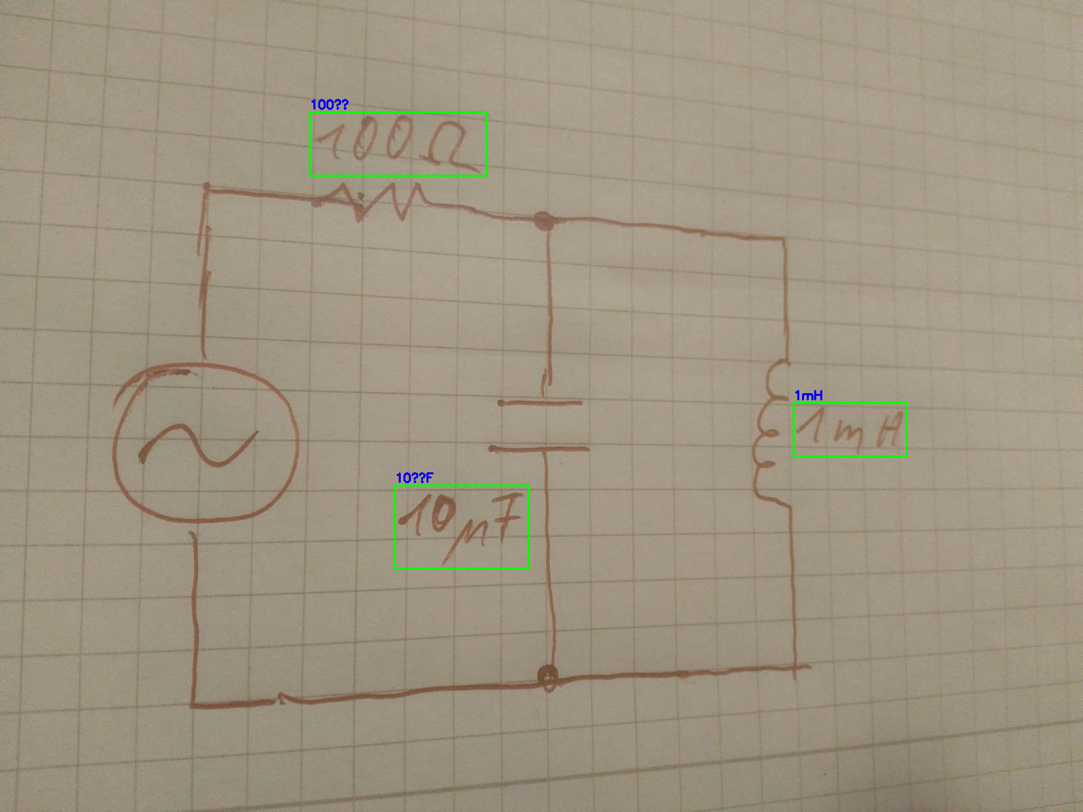
\includegraphics[width=\textwidth]{src/images/figures/text_detection_recognition2.png}
    \caption{Text Detection and Recognition (ii)}
    \label{fig:ocr-result-2}
\end{figure}

It is to be noted that the ``??'' shown in \cref{fig:ocr-result-1} and \cref{fig:ocr-result-2} is a limitation of the picture-rendering library used (OpenCV, Matplotlib), rather than a limitation of the \gls{ocr} model. The \gls{ocr} model accurately identifies symbols like $\mu$ (micro).

\subsection{Training Loss Curve}

% Due to the limitation of unpaid versions of cloud-based services like Google Colab and Lightning \gls{ai}, only 29 training epochs were successfully run. However, the results in those 29 epochs also seem promising as the training loss steadily decreased.
\cref{fig:ocr-training-loss} shows that the training loss decreases consistently throughout the 50 epochs, indicating the model is effectively memorizing the training data. However, the validation loss only drops until around 15-20 epochs before gradually increasing, indicating overfitting. Overfitting is an issue to be eradicated using extensive training using diverse datasets (either by addition of other datasets in training and/or augmentation). If the performance is considered satisfactory after training for only 15-20 epochs, early stopping may also be used.
\begin{figure}[H]
    \centering
    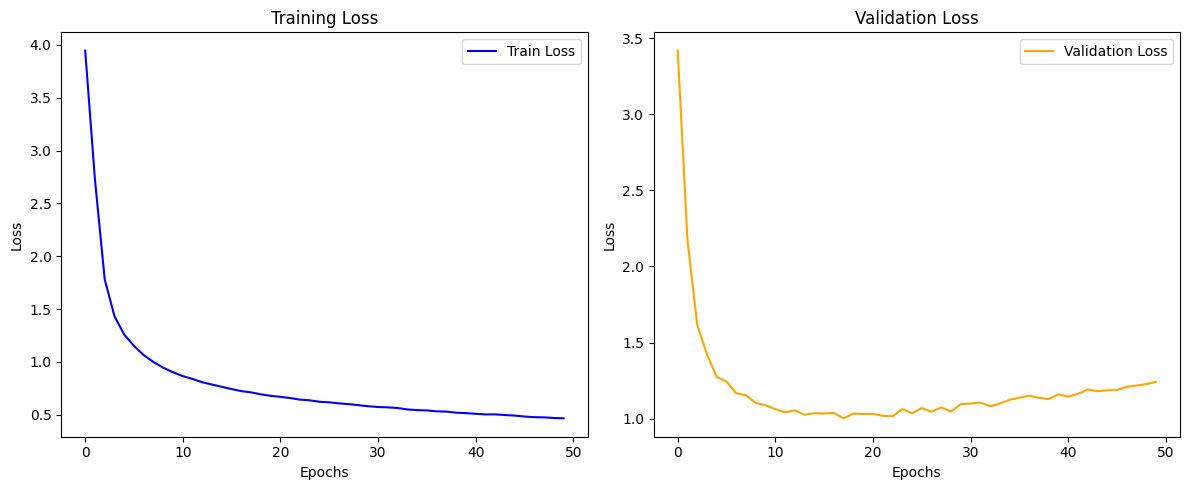
\includegraphics[width=\textwidth]{src/images/figures/OCR_loss_curve.png}
    \caption{Training Loss vs Epochs (\gls{ocr})}
    \label{fig:ocr-training-loss}
\end{figure}

\subsection{OCR Prediction}

% Due to the limitation of unpaid versions of cloud-based services like Google Colab and Lightning \gls{ai}, only 29 training epochs were successfully run. However, the results in those 29 epochs also seem promising as the training loss steadily decreased.
The predictions made by the OCR model for a random sample of test data is shown in \cref{fig:ocr-predictions}. The OCR model accurately recognizes the easily discernible text but is fallible in some cases. However, in this random sample of images, all the problem images (i.e. the ones OCR cannot recognize) are indiscernible to human eyes as well. For instance, the input image samples for GT: D5 and GT: 31 are completely black suggesting a preprocessing or cropping bug rather than a fault in the model.
\begin{figure}[H]
    \centering
    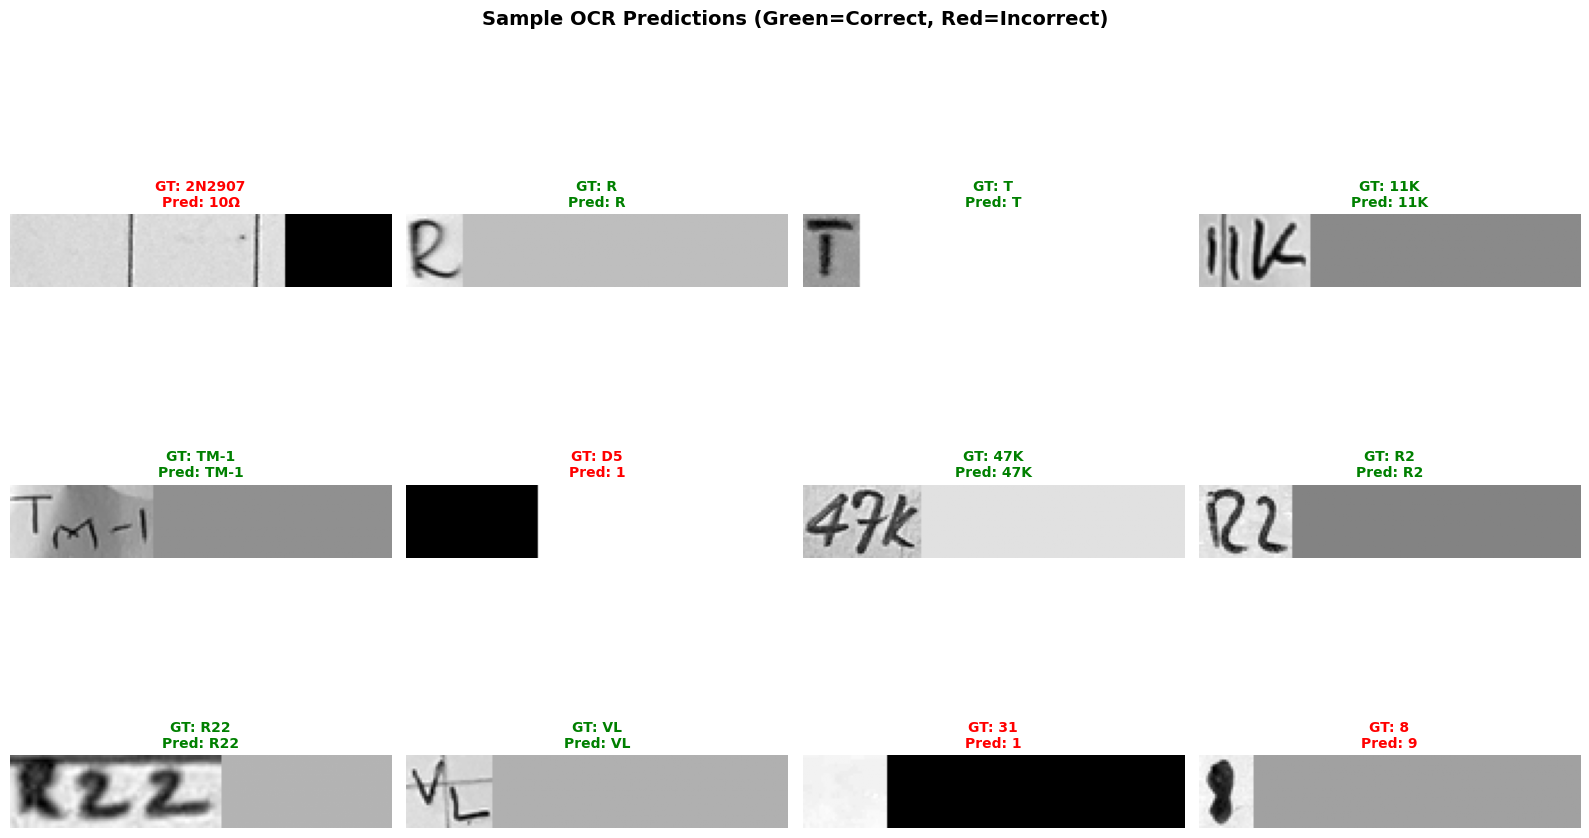
\includegraphics[width=\textwidth]{src/images/figures/ocr_test.png}
    \caption{OCR Model Predictions}
    \label{fig:ocr-predictions}
\end{figure}

\subsection{OCR Performance Analysis}
\cref{fig:ocr-performance-metrics} is a combination of images showing the performance metrics for the OCR model. The accuracy is 65.96\% and while this may seem low, the sample images reveal that accuracy might have taken a hit due to data corruption in the cropping process or preprocessing. Once this bug is somewhat fixed, accuracy is expected to rise. That being said, to improve the accuracy further, the task of refining the model, regardless of data corruption will continue. Likewise, the CER of 0.25 means that on average, 1 out of every 4 characters is predicted incorrectly. However, the histogram shows a notable bump at 1.0 (complete failure) confirming the presence of "garbage" inputs (like black boxes, as seen in the sample images). WER is shown to be 0.34. Its distribution is inherently binary because the model either gets the full component value right (WER being 0) or gets it wrong (WER = 1).
\begin{figure}[H]
    \centering
    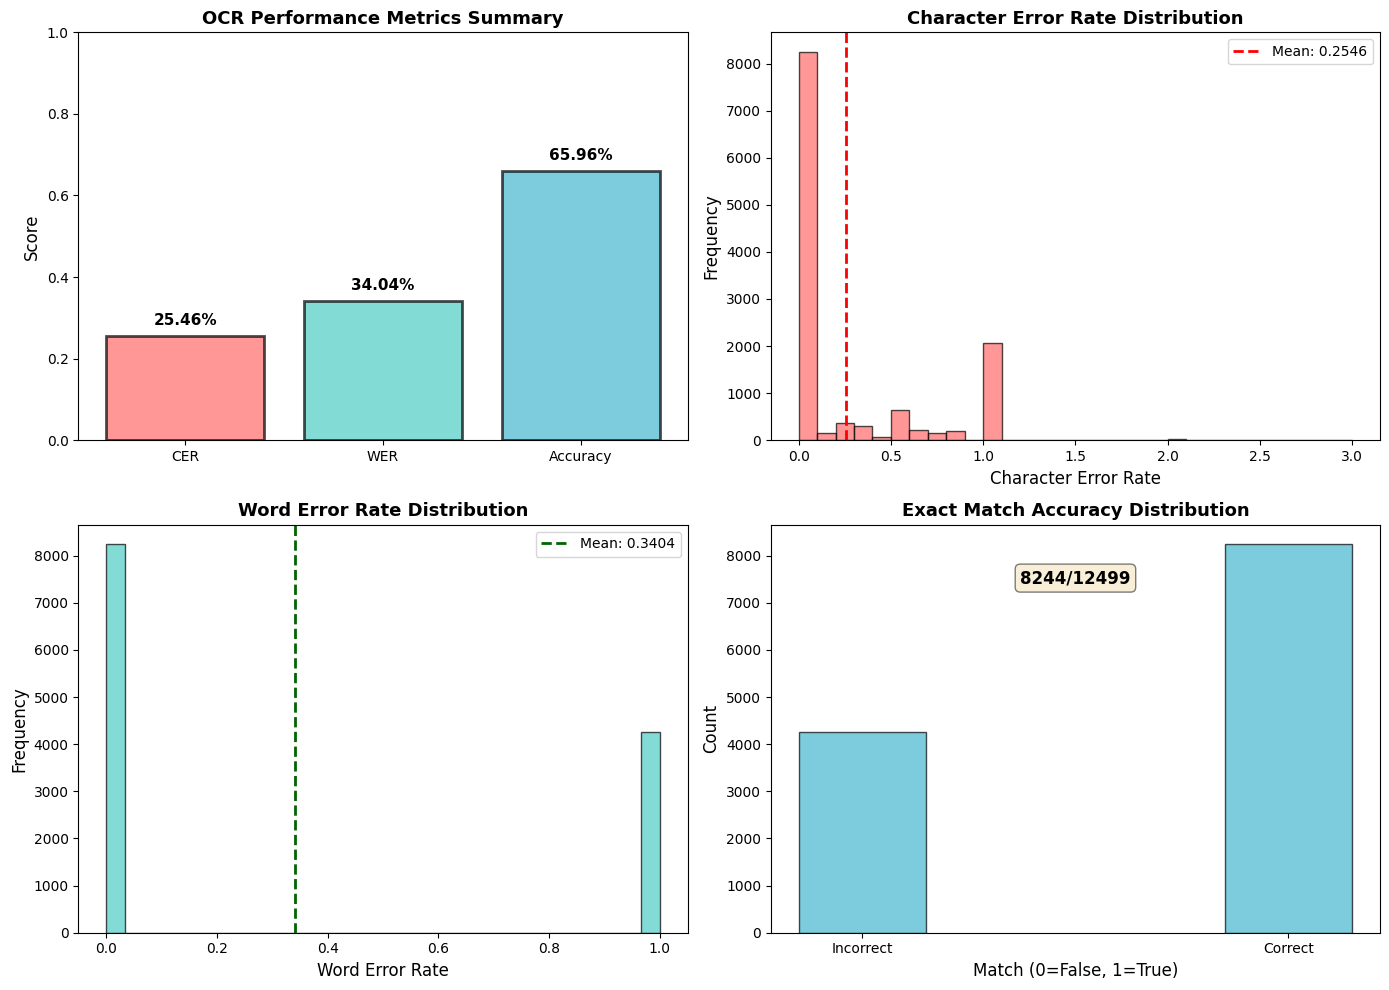
\includegraphics[width=\textwidth]{src/images/figures/cer_wer.png}
    \caption{OCR Performance Metrics and their Distributions}
    \label{fig:ocr-performance-metrics}
\end{figure}

\section{Junction-Based Wire Detection}

This section presents the experimental results obtained from the proposed junction-based wire detection pipeline applied to circuit diagram images. Each processing stage is evaluated independently and supported with quantitative measurements and visual evidence.

\subsection{Input Image and Preprocessing}

The experiment begins with a high-resolution scanned circuit diagram used as the input image. The original image dimensions are reported in terms of width and height in pixels to establish spatial scale consistency throughout the pipeline.

To enhance structural features and suppress background noise, the input image is converted to grayscale. Otsu's global thresholding method is then applied to automatically compute an optimal threshold value that separates foreground circuit elements from the background. The resulting binary image preserves wires, junctions, and components while eliminating illumination variations.

\begin{figure}[H]
    \centering
    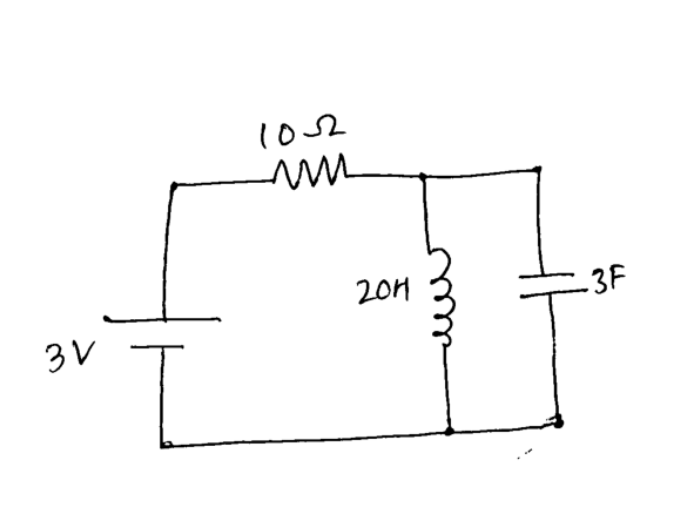
\includegraphics[width=\textwidth]{src/images/figures/otsu_thresholding.png}
    \caption{Otsu's Global Thresholding}
    \label{fig:otsu-thresholding}
\end{figure}

\subsection{Skeletonization}

Morphological skeletonization is applied to the binary image to reduce all wire segments to single pixel-wide centerlines. This transformation significantly reduces the number of foreground pixels while preserving the topological connectivity of the circuit network.

The reduction in foreground pixel count before and after skeletonization is recorded to quantify structural simplification. Despite aggressive thinning, wire continuity and junction connectivity remain intact, making the skeleton suitable for graph-based analysis.

\begin{figure}[H]
    \centering
    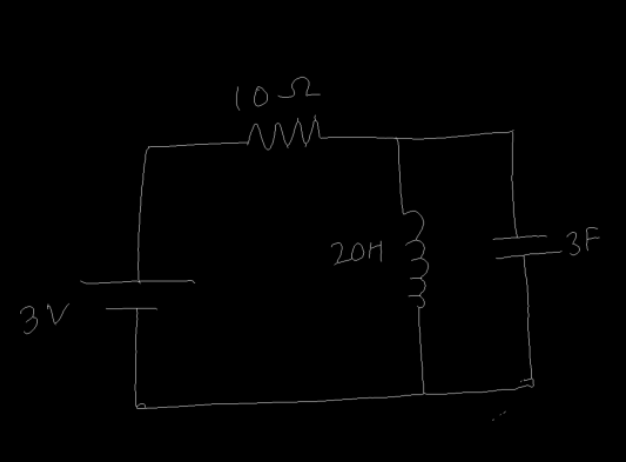
\includegraphics[width=\textwidth]{src/images/figures/skelotonization.png}
    \caption{Skeletonization}
    \label{fig:skeletonization}
\end{figure}

\subsection{Component Removal and Junction Isolation}

Object detection is performed using a trained \gls{yolo} model to identify and localize elements in the circuit diagram. Detected objects are classified as follows: Class 0 corresponds to text annotations, Class 1 corresponds to junctions, and all remaining classes correspond to circuit components.

The total number of detected objects per class is reported. To isolate only the wire network, bounding boxes associated with non-junction classes are removed from the skeleton image. This step eliminates component shapes while preserving junction points and interconnecting wires.

\begin{figure}[H]
    \centering
    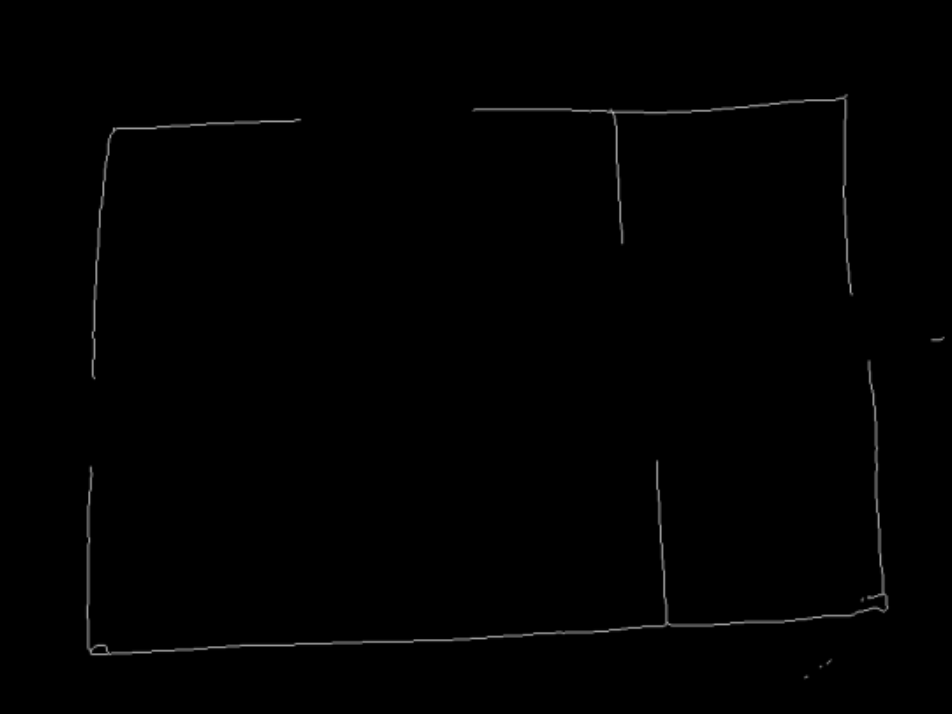
\includegraphics[width=\textwidth]{src/images/figures/component_removal.png}
    \caption{Component Removal}
    \label{fig:component-removal}
\end{figure}

\subsection{Junction Extraction and Wire Classification}

All detected junctions belonging to Class 1 (junctions) are extracted and their coordinates are converted from normalized \gls{yolo} format to pixel coordinates.

Each junction pair is classified based on geometric alignment. Pairs aligned horizontally are labeled as horizontal wires, pairs aligned vertically are labeled as vertical wires, and diagonally aligned pairs are rejected. The total number of accepted and rejected pairs is reported. Sample coordinate transformations from normalized values to pixel coordinates are also presented.

\begin{figure}[H]
    \centering
    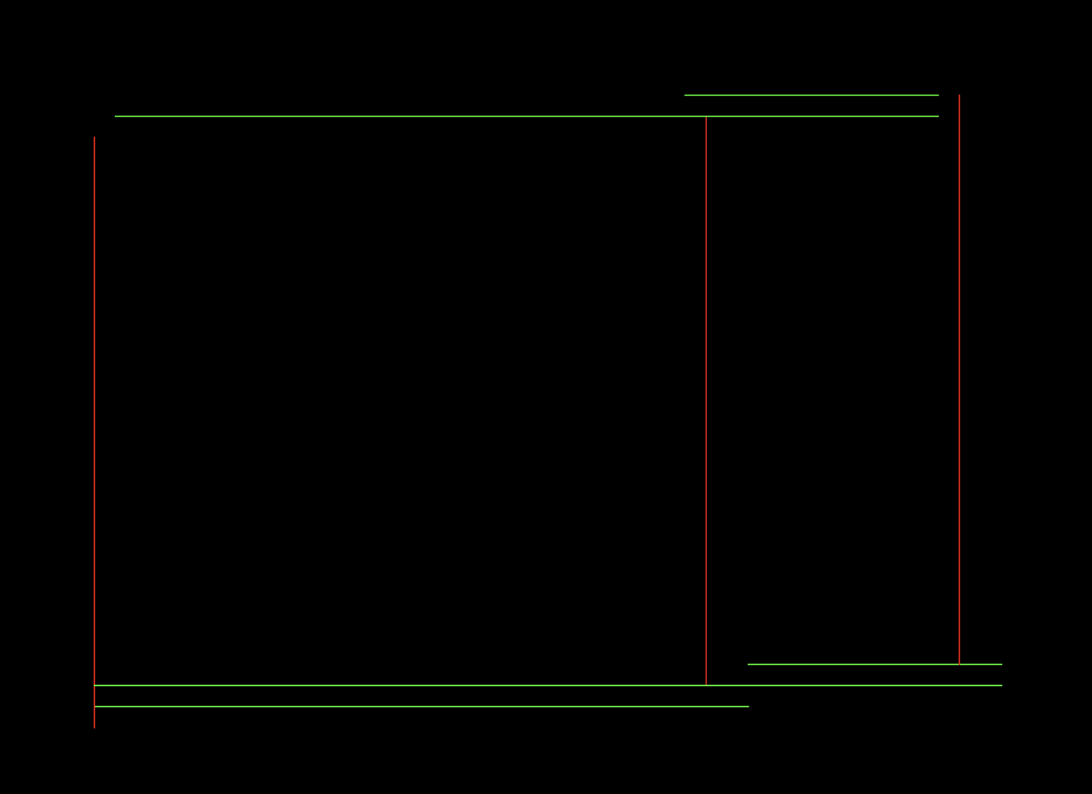
\includegraphics[width=\textwidth]{src/images/figures/wire_classification.png}
    \caption{Wire Classification}
    \label{fig:wire-classification}
\end{figure}

\subsection{Segment Consolidation Through Merging}

Initial wire detection may produce fragmented segments representing portions of the same physical wire. To address this, a merging algorithm is applied based on axis alignment tolerance of 16 pixels and overlapping or adjacent segment conditions.

The total number of raw wire segments before merging and the consolidated count after merging are reported.

\begin{figure}[H]
    \centering
    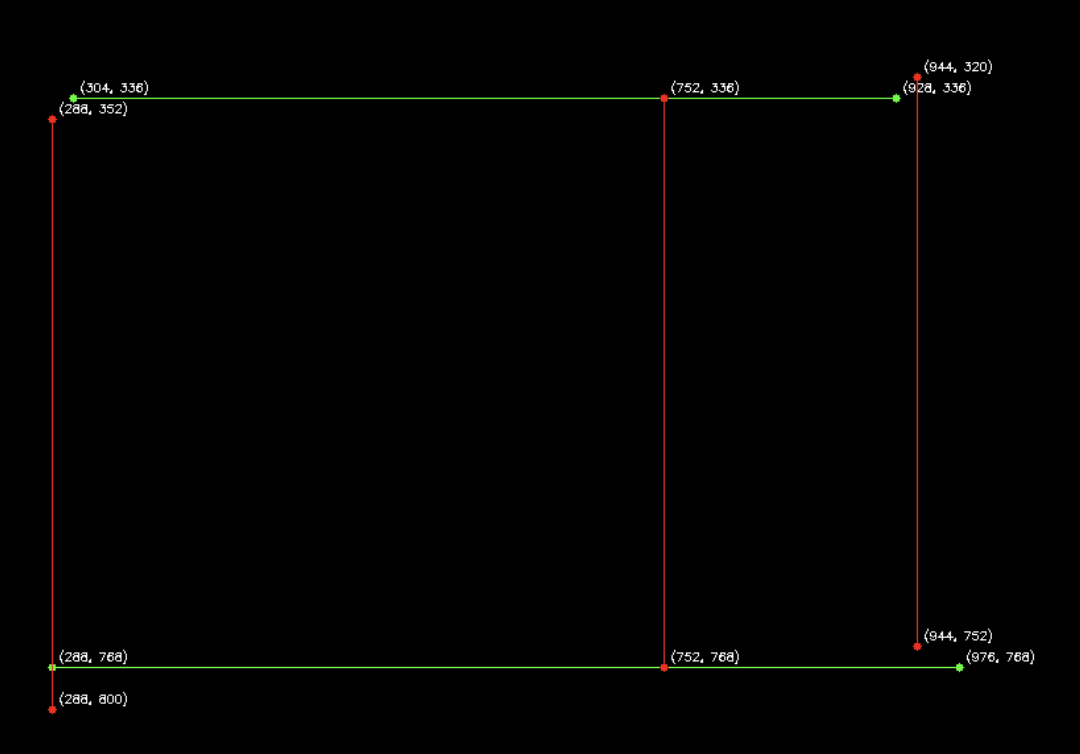
\includegraphics[width=\textwidth]{src/images/figures/segment_consolidation.png}
    \caption{Segment Consolidation Through Merging}
    \label{fig:segment-consolidation}
\end{figure}

\subsection{Component Bounding Box Overlay}

To enhance visualization and verify correct detection, component bounding boxes detected by \gls{yolo} are overlaid on the original circuit diagram. This overlay confirms that all circuit elements have been properly identified and localized, with bounding boxes accurately delineating component boundaries.

\begin{figure}[H]
    \centering
    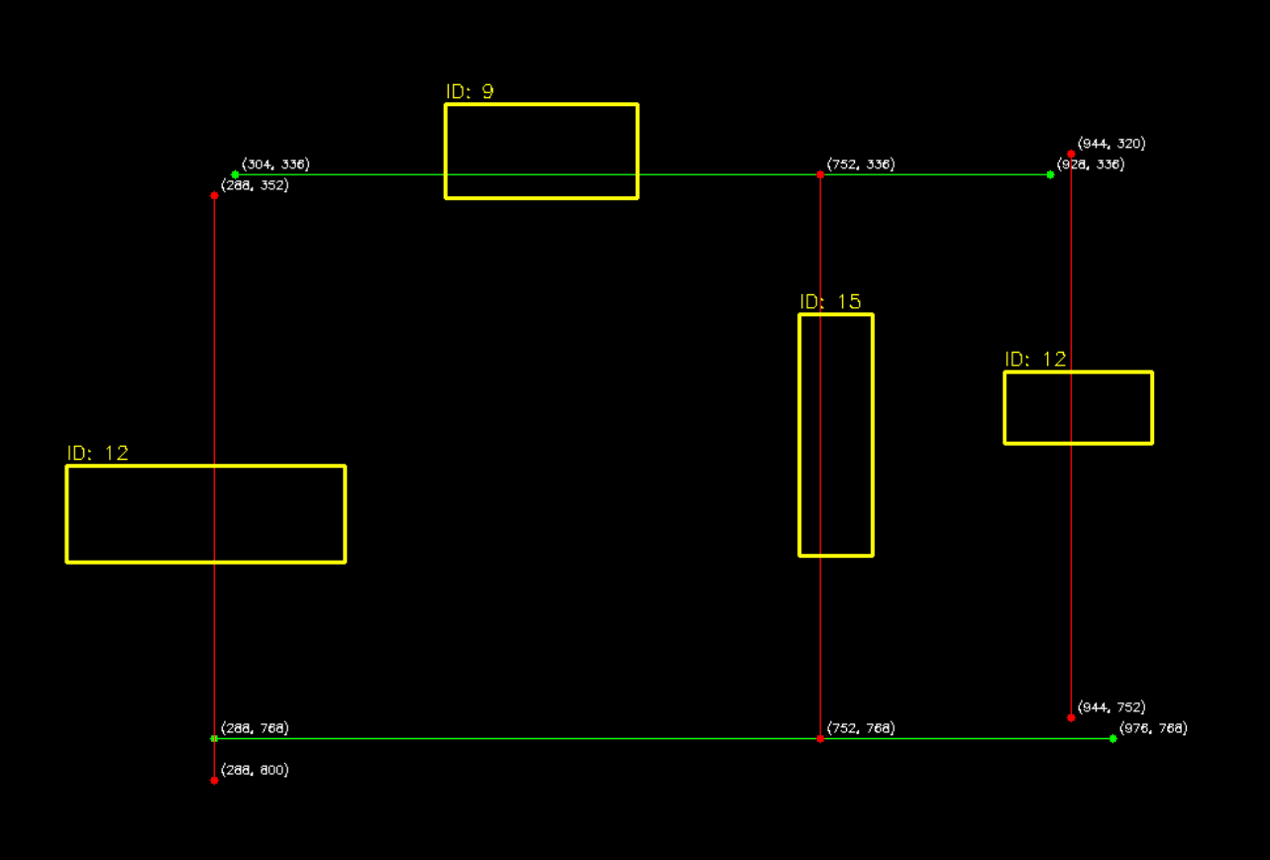
\includegraphics[width=\textwidth]{src/images/figures/bounding_box_overlay.png}
    \caption{Bounding Box Overlay}
    \label{fig:bbox-overlay}
\end{figure}

\subsection{Wire-Component Intersection Detection}

Intersection points between wires and component bounding box edges are computed to identify electrical connectivity. The total number of intersection points is reported along with a directional breakdown for horizontal and vertical wires intersecting specific component edges.

These intersections form the basis for reconstructing circuit connectivity graphs and netlists.

\begin{figure}[H]
    \centering
    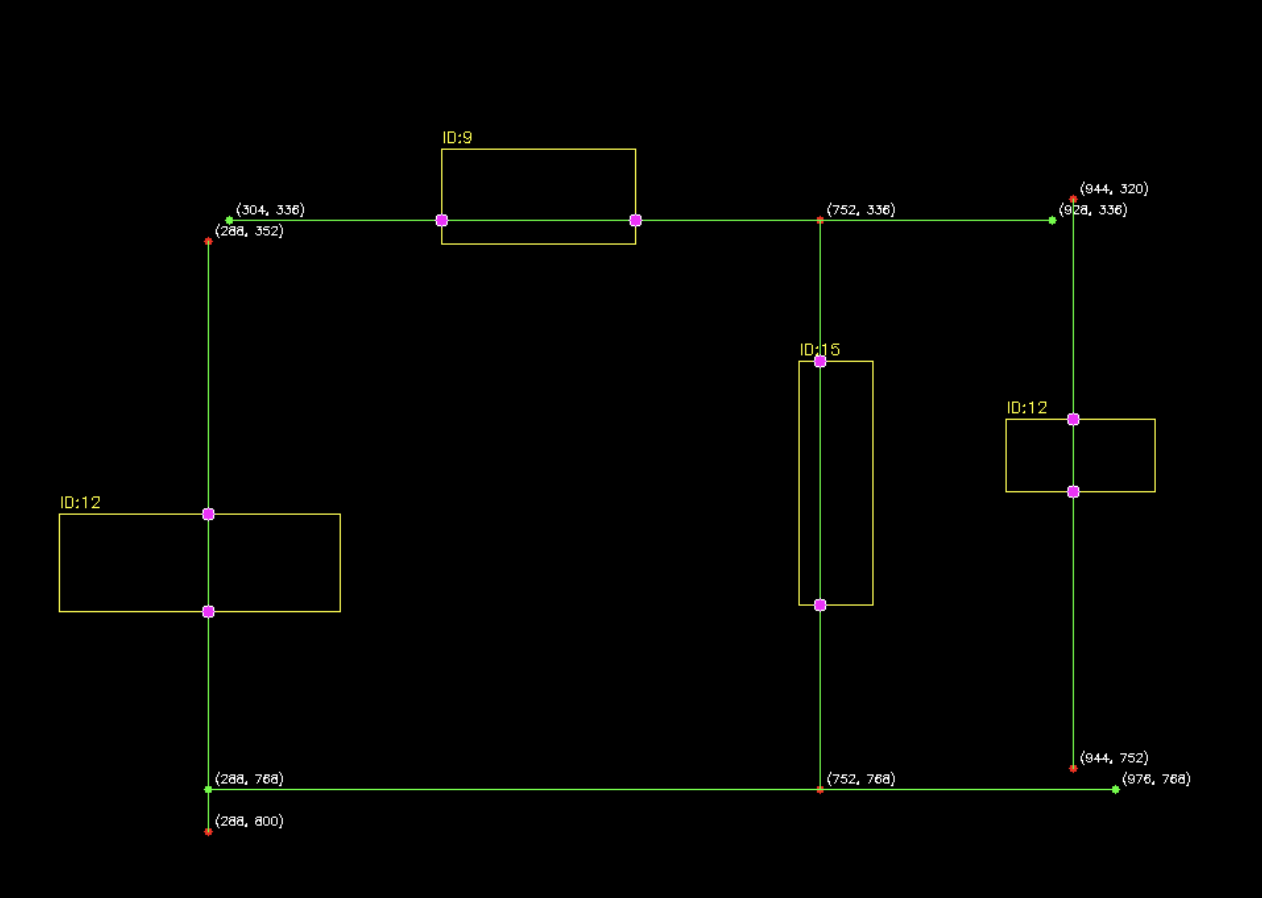
\includegraphics[width=\textwidth]{src/images/figures/wire_component_intersection_detection.png}
    \caption{Wire-Component Intersection Detection}
    \label{fig:wire-component-intersection}
\end{figure}

\section{Line Detection via Path Finding Visualization}

The algorithm produces visual outputs that demonstrate the effectiveness of the endpoint detection and graph construction pipeline. The following subsections present the key visualizations obtained from applying the Multi-Head BFS algorithm to the skeletonized circuit image.

\subsection{Skeletonized Image with Detected Endpoints}

Figure~\ref{fig:skeleton_endpoints} displays the skeletonized image with all detected endpoints overlaid. The skeleton representation captures the one-pixel-wide structure of the circuit lines after morphological processing. Red circles indicate the detected endpoints, which were identified using the bounding box intersection method for line segments and center-snapping for junction points. Green rectangles show the original YOLO bounding boxes used for endpoint localization. This visualization confirms that the endpoint detection algorithm successfully identifies connection points at the boundaries of detected objects.

\begin{figure}[H]
    \centering
    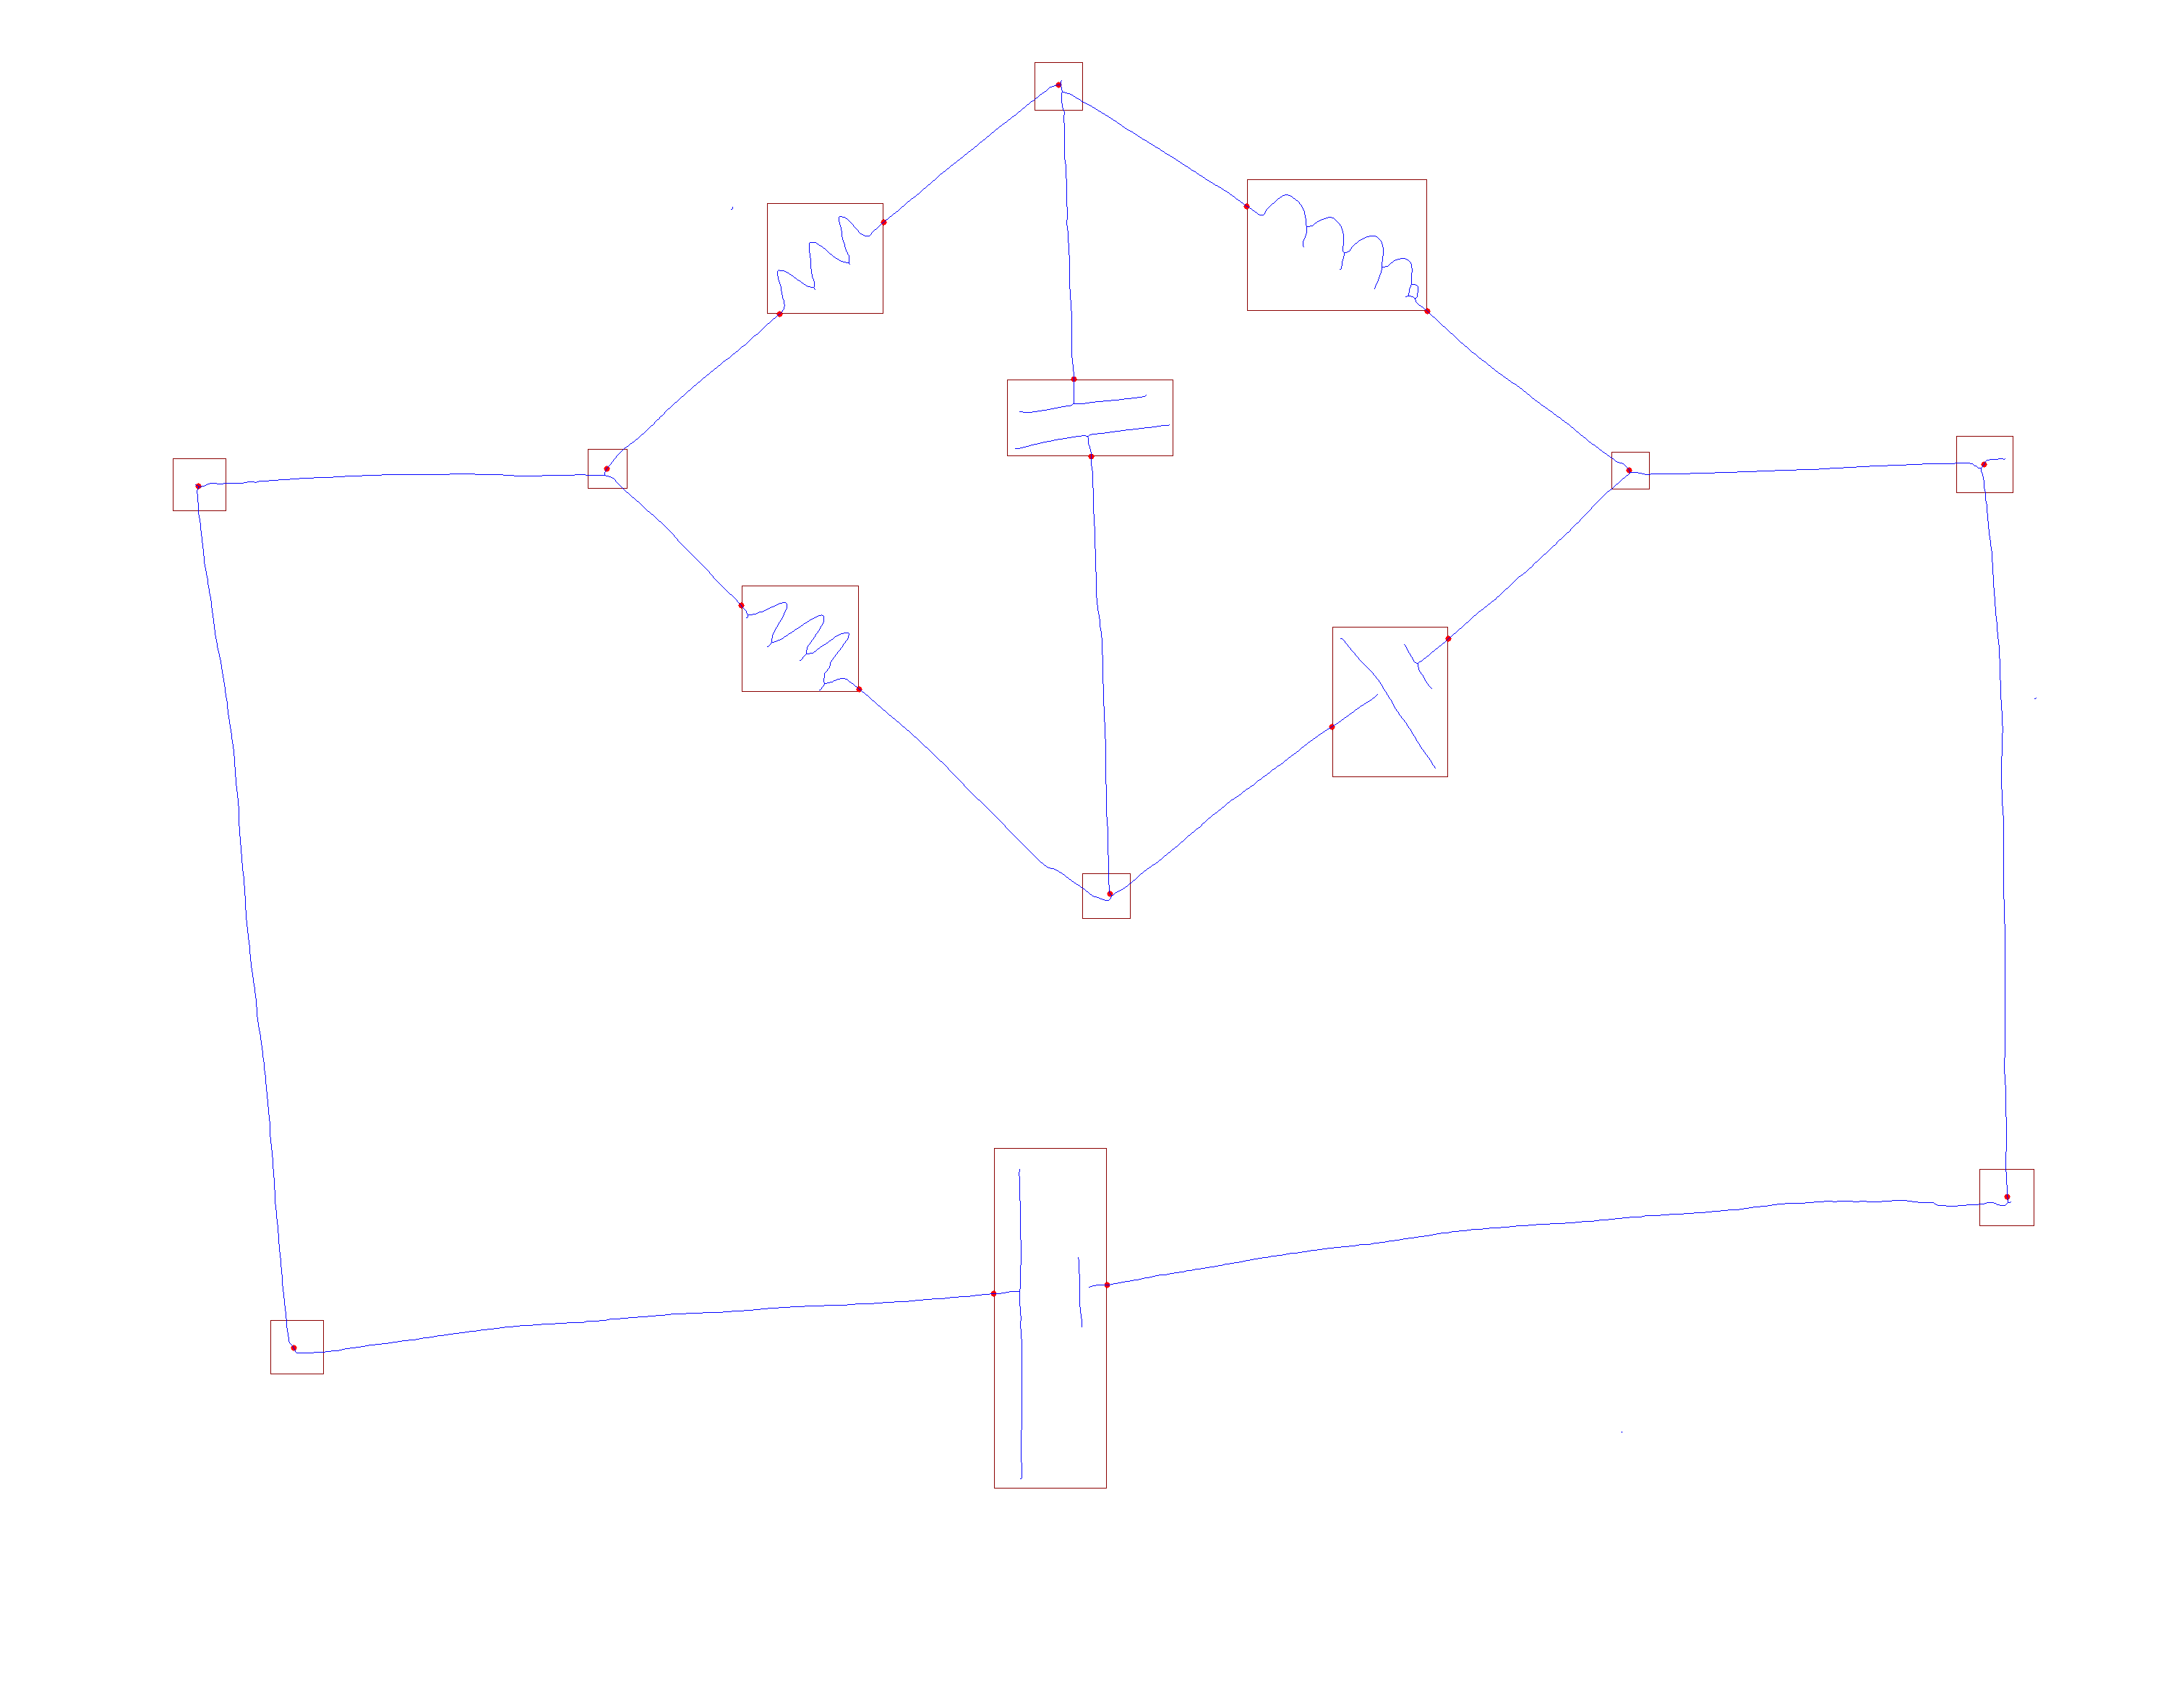
\includegraphics[width=0.8\textwidth]{src/images/figures/skeleton_with_endpoints.png}
    \caption{Skeletonized image with detected endpoints}
    \label{fig:skeleton_endpoints}
\end{figure}

\subsection{Adjacency Graph Visualization}

Figure~\ref{fig:adjacency_graph} presents the final adjacency graph constructed using the Multi-Head BFS algorithm. Each node corresponds to a detected endpoint from the previous stage. Blue lines connecting the nodes represent edges in the graph, indicating skeleton connectivity between endpoints. The graph has been processed to remove self-edges (connections between endpoints belonging to the same detected object), ensuring that only meaningful inter-component connections are preserved. This graph structure enables downstream applications such as circuit topology analysis and netlist extraction.

\begin{figure}[H]
    \centering
    
\includegraphics[width=0.7\textwidth]{src/images/figures/adjacency_graph.png}
    \caption{Adjacency graph constructed using Multi-Head BFS algorithm}
    \label{fig:adjacency_graph}
\end{figure}

\section{Frontend Visualization}

The frontend of the \gls{circuitron} web application provides an interactive environment for circuit design, simulation, and analysis. It enables users to construct electrical circuits using a drag-and-drop schematic editor with grid-based alignment, snap-to-grid functionality, and real-time wire routing. Components such as passive elements, active devices, and sources can be configured through a properties panel that allows precise control over electrical parameters and placement. 

The system integrates simulation controls for transient analysis, allowing users to define time parameters, execute simulations, and visualize results through dynamically rendered voltage-time plots. Measurement probes support real-time signal monitoring with automated computation of key metrics, including maximum, minimum, peak-to-peak range, and \gls{rms} values. Additionally, the frontend supports exporting simulation data and visualizations in standard formats, enabling seamless documentation and further offline analysis.

\begin{figure}[H]
    \centering
    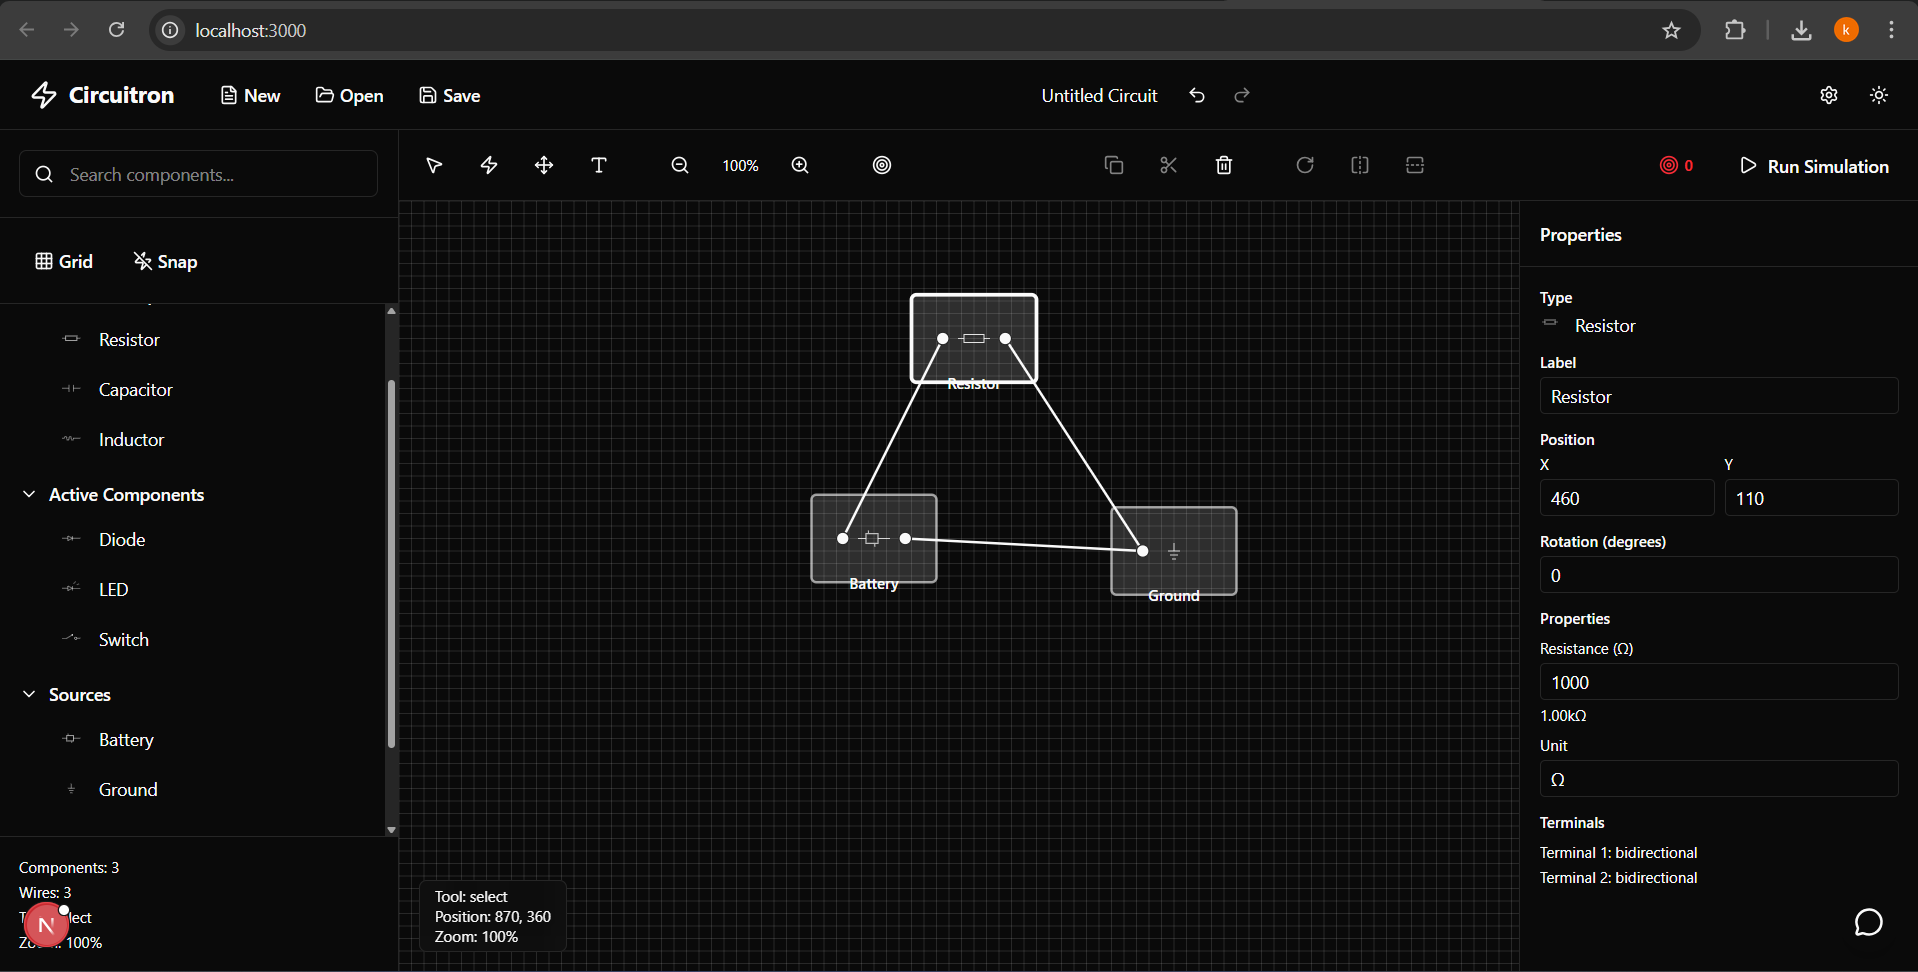
\includegraphics[width=\textwidth]{src/images/figures/frontend_circuit.png}
    \caption{Digitally Drawn Circuit}
    \label{fig:digital-circuit-editor}
\end{figure}

\begin{figure}[H]
    \centering
    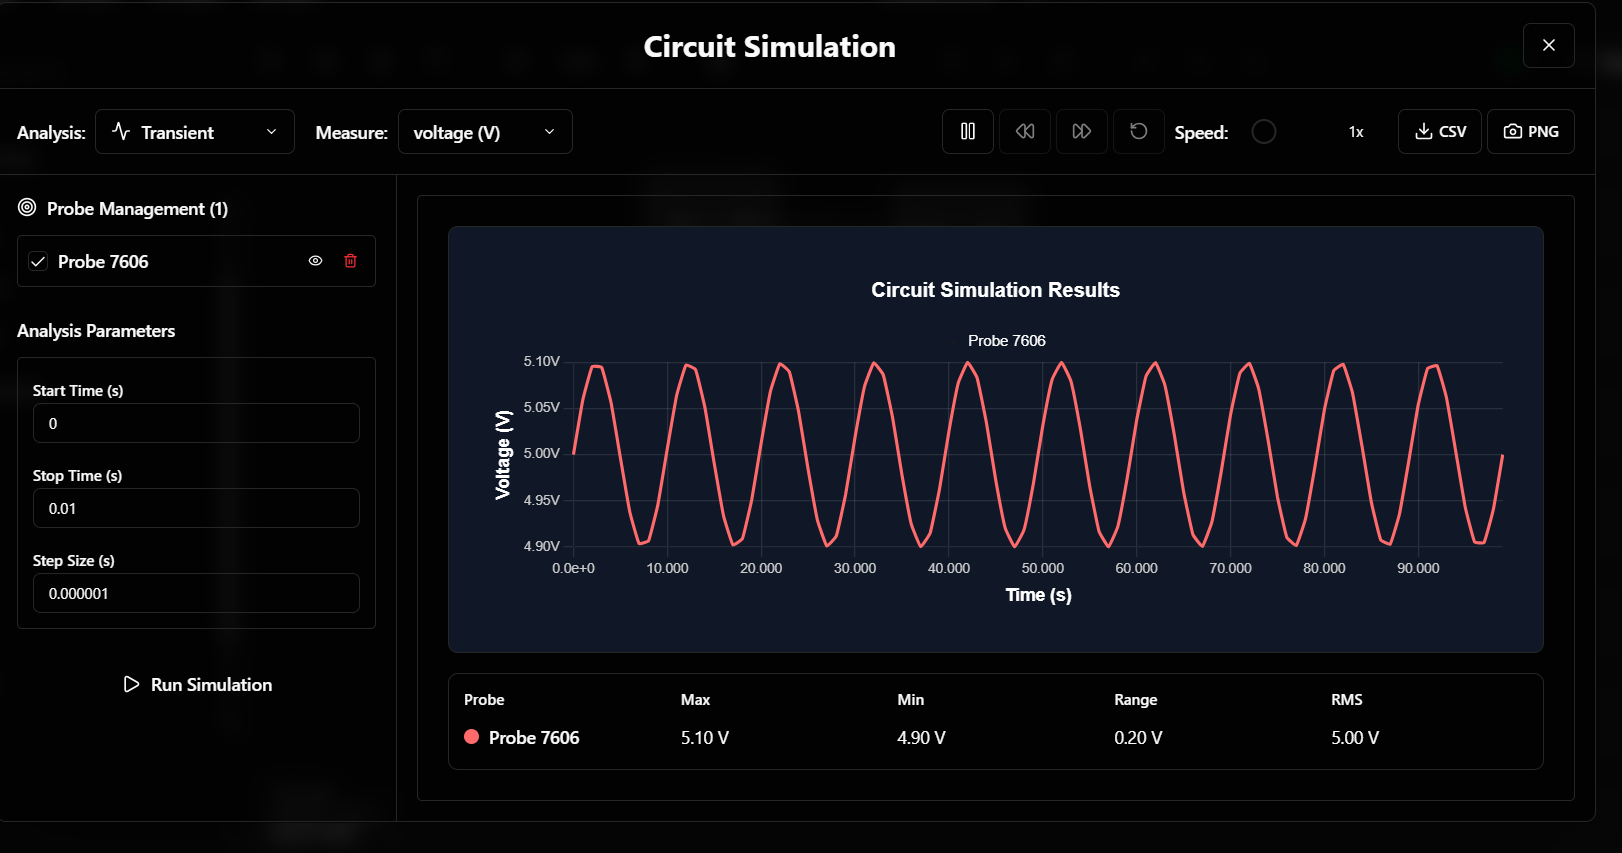
\includegraphics[width=\textwidth]{src/images/figures/frontend_simulation.png}
    \caption{Example Circuit Simulation Result}
    \label{fig:simulation-result}
\end{figure}

\chapter{REMAINING TASKS}

As of yet, the individual component/text detection and extraction elements along with node detection and wire connectivity seem to be working. Component detection with fine-tuned YOLOv7 model, text extraction using custom OCR model trained from scratch (working in tandem), and path finding-based wire detection have been achieved. Moreover, these separate modules have been successfully integrated to build a complete project pipeline that takes an image of a circuit and gives out the simulation graphs after selected simulation type (transient analysis, constant voltage analysis, etc). While work on improving the accuracy and robustness of the models will definitely continue in the background until the target values for metrics are reached, the primary goal is to add a few user-focused features. LLM-integration (Gemini) is a major task remaining. Such an LLM-based question-and-answer feature enables users to interact with the system, ask questions about the circuit, and receive direct feedback and analysis based on the simulation results. Integration of authentication and database in the project pipeline is the next step as a facilitating step for users to save a particular circuit for future use. Other minor remaining tasks include effective integration of the built APIs with the frontend of the web-app, and general refinement duties. This leaves the hosting part. For hosting, if possible, a free service (Vercel or Python Anywhere) may be used, or a paid service (Microsoft Azure) can be used.

\section{Summary of Remaining Tasks}

\begin{table}[H]
    \centering
    \small
    \caption{Summary of Remaining Tasks}
    \begin{tabular}{lll}
        \toprule
        \textbf{SN} & \textbf{Modules} & \textbf{Remarks} \\
        \midrule
        1 & LLM Integration & Gemini integration for question-and-answer feature \\
        2 & Authentication and Database & For saving and retrieving circuits for future use \\
        3 & API and Frontend Integration & Effective integration of built APIs with web-app \\
        4 & System Refinement & General refinement and optimization duties \\
        5 & Hosting and Deployment & Free (Vercel, PythonAnywhere) or paid (Azure) services \\
        \bottomrule
    \end{tabular}
    \label{tab:remaining-tasks-summary}
\end{table}


% \noindent\textbf{CHAPTER GUIDE:} Purpose: describe unfinished work, risks, and a realistic plan. Must include: What is completed vs pending, Remaining milestones, Risks/blockers + mitigation. LaTeX: Use itemize for checklists; enumerate for ordered milestones.

% \section{Comparative Analysis of Object Detection using YOLOv5 and YOLOv7}

% \subsection{Confusion Matrix}

% To assess per-class performance, confusion matrices were generated using the validation set.

% \begin{figure}[htbp]
%     \centering
%     \fbox{\parbox{0.85\textwidth}{\centering [Figure Placeholder 6-13: Confusion Matrix for YOLOv5 showing per-class detection performance and misclassification patterns]}}
%     \caption{Confusion Matrix for YOLOv5}
%     \label{fig:confusion-matrix-v5-rt}
% \end{figure}

% \begin{figure}[htbp]
%     \centering
%     \fbox{\parbox{0.85\textwidth}{\centering [Figure Placeholder 6-14: Confusion Matrix for YOLOv7 demonstrating improved class separation and fewer misclassifications]}}
%     \caption{Confusion Matrix for YOLOv7}
%     \label{fig:confusion-matrix-v7-rt}
% \end{figure}

% \subsection{Quantitative Results Comparison}

% Final epoch results show \gls{yolo}v7 outperformed \gls{yolo}v5 across all major metrics.

% \begin{table}[htbp]
%     \centering
%     \caption{Comparison of Performance Metrics for YOLOv5 and YOLOv7}
%     \label{table:yolo-comparison-rt}
%     \begin{tabular}{lrr}
%         \toprule
%         \textbf{Metric} & \textbf{YOLOv5} & \textbf{YOLOv7} \\
%         \midrule
%         \gls{map}@0.5 & 0.61 & 0.83 \\
%         \gls{map}@0.5:0.95 & 0.41 & 0.60 \\
%         Precision & 0.84 & 0.93 \\
%         Recall & 0.62 & 0.78 \\
%         Epochs Trained & 200 & 100 \\
%         \bottomrule
%     \end{tabular}
% \end{table}

% Overall, \gls{yolo}v7 showed a clear advantage over \gls{yolo}v5 in our experiments. It not only achieved higher values for precision, recall, and mean average precision but also required fewer epochs to converge. \gls{yolo}v7's confusion matrix reflected better class separation and fewer misclassifications. The improvements in F1 score and overall stability of predictions across confidence thresholds make \gls{yolo}v7 a more robust choice for circuit diagram interpretation.

% \section{\gls{ocr} Results}

% The out-of-the-box default \gls{easyocr} implementation without fine-tuning was able to detect some of the component values from the circuit; however, the results left a lot to be desired. This made it clear that proper training of the recognition model is absolutely essential for this project.

% After training the text recognition model from scratch, results were much improved. Two randomly picked images from the dataset are shown below after passing through the detection (\gls{yolo}v7) and recognition (\gls{ocr}) models.

% \begin{figure}[htbp]
%     \centering
%     \fbox{\parbox{0.85\textwidth}{\centering [Figure Placeholder 6-15: Text Detection and Recognition (i) showing circuit component values accurately extracted from handwritten diagrams]}}
%     \caption{Text Detection and Recognition (i)}
%     \label{fig:ocr-result-1-rt}
% \end{figure}

% \begin{figure}[htbp]
%     \centering
%     \fbox{\parbox{0.85\textwidth}{\centering [Figure Placeholder 6-16: Text Detection and Recognition (ii) demonstrating OCR model accuracy on diverse component labels]}}
%     \caption{Text Detection and Recognition (ii)}
%     \label{fig:ocr-result-2-rt}
% \end{figure}

% It is to be noted that the ``??'' shown in \cref{fig:ocr-result-1-rt} and \cref{fig:ocr-result-2-rt} is a limitation of the picture-rendering library used (OpenCV, Matplotlib), rather than a limitation of the \gls{ocr} model. The \gls{ocr} model accurately identifies symbols like $\mu$ (micro).

% \subsection{Training Loss Curve}

% Due to the limitation of unpaid versions of cloud-based services like Google Colab and Lightning \gls{ai}, only 29 training epochs were successfully run. However, the results in those 29 epochs also seem promising as the training loss steadily decreased.

% \begin{figure}[htbp]
%     \centering
%     \fbox{\parbox{0.85\textwidth}{\centering [Figure Placeholder 6-17: Training Loss vs Epochs (OCR) showing consistent convergence of the custom text recognition model]}}
%     \caption{Training Loss vs Epochs (\gls{ocr})}
%     \label{fig:ocr-training-loss-rt}
% \end{figure}

% \section{Junction-Based Wire Detection}

% This section presents the experimental results obtained from the proposed junction-based wire detection pipeline applied to circuit diagram images. Each processing stage is evaluated independently and supported with quantitative measurements and visual evidence.

% \subsection{Input Image and Preprocessing}

% The experiment begins with a high-resolution scanned circuit diagram used as the input image. The original image dimensions are reported in terms of width and height in pixels to establish spatial scale consistency throughout the pipeline.

% To enhance structural features and suppress background noise, the input image is converted to grayscale. Otsu's global thresholding method is then applied to automatically compute an optimal threshold value that separates foreground circuit elements from the background. The resulting binary image preserves wires, junctions, and components while eliminating illumination variations.

% \begin{figure}[htbp]
%     \centering
%     \fbox{\parbox{0.85\textwidth}{\centering [Figure Placeholder 6-18: Otsu's Global Thresholding showing binary conversion of circuit diagram with foreground-background separation]}}
%     \caption{Otsu's Global Thresholding}
%     \label{fig:otsu-thresholding-rt}
% \end{figure}

% \subsection{Skeletonization}

% Morphological skeletonization is applied to the binary image to reduce all wire segments to single pixel-wide centerlines. This transformation significantly reduces the number of foreground pixels while preserving the topological connectivity of the circuit network.

% The reduction in foreground pixel count before and after skeletonization is recorded to quantify structural simplification. Despite aggressive thinning, wire continuity and junction connectivity remain intact, making the skeleton suitable for graph-based analysis.

% \begin{figure}[htbp]
%     \centering
%     \fbox{\parbox{0.85\textwidth}{\centering [Figure Placeholder 6-19: Skeletonization showing single pixel-wide wire representations while preserving junction connectivity]}}
%     \caption{Skeletonization}
%     \label{fig:skeletonization-rt}
% \end{figure}

% \subsection{Component Removal and Junction Isolation}

% Object detection is performed using a trained \gls{yolo} model to identify and localize elements in the circuit diagram. Detected objects are classified as follows: Class 0 corresponds to text annotations, Class 1 corresponds to junctions, and all remaining classes correspond to circuit components.

% The total number of detected objects per class is reported. To isolate only the wire network, bounding boxes associated with non-junction classes are removed from the skeleton image. This step eliminates component shapes while preserving junction points and interconnecting wires.

% \begin{figure}[htbp]
%     \centering
%     \fbox{\parbox{0.85\textwidth}{\centering [Figure Placeholder 6-20: Component Removal showing wire network isolation after removing component bounding boxes]}}
%     \caption{Component Removal}
%     \label{fig:component-removal-rt}
% \end{figure}

% \subsection{Junction Extraction and Wire Classification}

% All detected junctions belonging to Class 1 (junctions) are extracted and their coordinates are converted from normalized \gls{yolo} format to pixel coordinates.

% Each junction pair is classified based on geometric alignment. Pairs aligned horizontally are labeled as horizontal wires, pairs aligned vertically are labeled as vertical wires, and diagonally aligned pairs are rejected. The total number of accepted and rejected pairs is reported. Sample coordinate transformations from normalized values to pixel coordinates are also presented.

% \begin{figure}[htbp]
%     \centering
%     \fbox{\parbox{0.85\textwidth}{\centering [Figure Placeholder 6-21: Wire Classification showing horizontal, vertical, and rejected diagonal wire pairs]}}
%     \caption{Wire Classification}
%     \label{fig:wire-classification-rt}
% \end{figure}

% \subsection{Segment Consolidation Through Merging}

% Initial wire detection may produce fragmented segments representing portions of the same physical wire. To address this, a merging algorithm is applied based on axis alignment tolerance of 16 pixels and overlapping or adjacent segment conditions.

% The total number of raw wire segments before merging and the consolidated count after merging are reported.

% \begin{figure}[htbp]
%     \centering
%     \fbox{\parbox{0.85\textwidth}{\centering [Figure Placeholder 6-22: Segment Consolidation Through Merging demonstrating reduction of fragmented wire segments into coherent wires]}}
%     \caption{Segment Consolidation Through Merging}
%     \label{fig:segment-consolidation-rt}
% \end{figure}

% \subsection{Component Bounding Box Overlay}

% To enhance visualization and verify correct detection, component bounding boxes detected by \gls{yolo} are overlaid on the original circuit diagram. This overlay confirms that all circuit elements have been properly identified and localized, with bounding boxes accurately delineating component boundaries.

% \begin{figure}[htbp]
%     \centering
%     \fbox{\parbox{0.85\textwidth}{\centering [Figure Placeholder 6-23: Bounding Box Overlay showing component detection boxes overlaid on original circuit diagram]}}
%     \caption{Bounding Box Overlay}
%     \label{fig:bbox-overlay-rt}
% \end{figure}

% \subsection{Wire-Component Intersection Detection}

% Intersection points between wires and component bounding box edges are computed to identify electrical connectivity. The total number of intersection points is reported along with a directional breakdown for horizontal and vertical wires intersecting specific component edges.

% These intersections form the basis for reconstructing circuit connectivity graphs and netlists.

% \begin{figure}[htbp]
%     \centering
%     \fbox{\parbox{0.85\textwidth}{\centering [Figure Placeholder 6-24: Wire-Component Intersection Detection showing computed connection points between wires and component boundaries]}}
%     \caption{Wire-Component Intersection Detection}
%     \label{fig:wire-component-intersection-rt}
% \end{figure}

% \section{Frontend Visualization}

% The frontend of the \gls{circuitron} web application provides an interactive environment for circuit design, simulation, and analysis. It enables users to construct electrical circuits using a drag-and-drop schematic editor with grid-based alignment, snap-to-grid functionality, and real-time wire routing. Components such as passive elements, active devices, and sources can be configured through a properties panel that allows precise control over electrical parameters and placement.

% The system integrates simulation controls for transient analysis, allowing users to define time parameters, execute simulations, and visualize results through dynamically rendered voltage-time plots. Measurement probes support real-time signal monitoring with automated computation of key metrics, including maximum, minimum, peak-to-peak range, and \gls{rms} values. Additionally, the frontend supports exporting simulation data and visualizations in standard formats, enabling seamless documentation and further offline analysis.

% \begin{figure}[htbp]
%     \centering
%     \fbox{\parbox{0.85\textwidth}{\centering [Figure Placeholder 6-25: Digitally Drawn Circuit showing the drag-and-drop schematic editor interface with grid-based component placement and real-time wire routing]}}
%     \caption{Digitally Drawn Circuit}
%     \label{fig:digital-circuit-editor-rt}
% \end{figure}

% \begin{figure}[htbp]
%     \centering
%     \fbox{\parbox{0.85\textwidth}{\centering [Figure Placeholder 6-26: Example Circuit Simulation Result displaying voltage-time plots with measurement probes showing maximum, minimum, peak-to-peak, and RMS values]}}
%     \caption{Example Circuit Simulation Result}
%     \label{fig:simulation-result-rt}
% \end{figure}


% \input{src/chapters/conclusion}

% =====================
% BACKMATTER / APPENDICES
% =====================
\clearpage
\chapter{APPENDICES}
% include the page wise photos of plagarism summary document:
% \chapter{MATHEMATICAL DERIVATIONS}
% You can include the Derivation and mathematical part of your project that is not necessary to be included in the main report here. To provide reader with the complete mathematical background of your project, you can include the derivations, proofs, and detailed explanations of theorems or formulas used in your project. and then you can cross reference them in the main report.
% \section{Proof of Theorem 1:} Convex Optimization Problem can be solved using Gradient Descent Method.
% \section{Proof of Theorem 2:} Convergence of Gradient Descent Method for Convex Functions.
% \section{Gaussian Distribution} 
% The Gaussian distribution, also known as the normal distribution, is a continuous probability distribution characterized by its bell-shaped curve. It is defined by its mean ($\mu$) and standard deviation ($\sigma$). The probability density function (PDF) of a Gaussian distribution is given by:
% \[
% f(x) = \frac{1}{\sigma\sqrt{2\pi}} \exp\!\left(-\frac{(x-\mu)^2}{2\sigma^2}\right).
% \]



\section*{Appendix A: Budget Estimation}
\addcontentsline{toc}{section}{Appendix A: Budget Estimation}
The total budget required for the successful completion of the project is estimated to be NPR 41,160. This budget covers various aspects of the project, including computation resources, cloud services, IEEE membership, and miscellaneous expenses.

\subsection*{Cost Estimation Breakdown}

\begin{table}[H]
    \centering
    \small
    \caption{Project Budget Breakdown}
    \begin{tabular}{p{3.5cm}p{5.5cm}c}
        \toprule
        \textbf{Category} & \textbf{Details} & \textbf{Estimated Cost (NPR)} \\
        \midrule
        Computation Requirements & Google Colab Pro (\$9.99 per month), NVIDIA T4 GPU (\$0.35 per hour), Lightning AI Credits & 20,000 \\
        Cloud Service and Hosting & Domain Registration (\$12), Cloud Storage 100 GB (\$3 per month), Database hosting (\$30-\$50 per month) & 4,000 \\
        IEEE Xplore Membership & Annual subscription for accessing research articles, journals & 2,160 \\
        Miscellaneous Costs & Report printing, binding, API, etc. & 15,000 \\
        \midrule
        Total & & \textbf{41,160} \\
        \bottomrule
    \end{tabular}
    \label{tab:project_budget}
\end{table}

% \section{Bill of Materials (BOM)}
% Keep this only if relevant to your project.
% This section details all components that will be integrated into the final product/system. These are the materials that constitute the deliverable hardware (if any).

% \begin{table}[H]
%     \centering
%     \small
%     \caption{Bill of Materials}
%     \begin{tabular}{p{3cm}p{4cm}ccc}
%         \toprule
%         \textbf{Component}                    & \textbf{Specification} & \textbf{Qty} & \textbf{Unit Cost} & \textbf{Total} \\
%         \midrule
%         Microcontroller                       & ESP32 DevKit           & 1            & \$10               & \$10           \\
%         Sensor                                & DHT22 Sensor           & 2            & \$5                & \$10           \\
%         Actuator                              & Servo Motor SG90       & 2            & \$3                & \$6            \\
%         Power Supply                          & 5V/2A Adapter          & 1            & \$8                & \$8            \\
%         PCB                                   & Custom PCB (100x100mm) & 1            & \$15               & \$15           \\
%         Enclosure                             & ABS Plastic Box        & 1            & \$12               & \$12           \\
%         \midrule
%         \multicolumn{4}{r}{\textbf{Subtotal}} & \textbf{\$61}                                                               \\
%         \bottomrule
%     \end{tabular}
%     \label{tab:bom}
% \end{table}

% \textit{Note: Replace the example entries above with actual components for your project.}

% \section{Software and Cloud Services}
% This section covers all software tools, cloud computing resources, and subscription services required for the project.

% \begin{table}[H]
%     \centering
%     \small
%     \caption{Software and Cloud Services Cost}
%     \begin{tabular}{p{3.5cm}p{5cm}p{2.5cm}}
%         \toprule
%         \textbf{Service}                              & \textbf{Description}                            & \textbf{Cost} \\
%         \midrule
%         Open-Source Software                          & Python, NumPy, SciPy, TensorFlow, PyTorch, etc. & Free          \\
%         Cloud Computing                               & Google Colab Pro (GPU access for training)      & \$10/month    \\
%         Cloud Storage                                 & Google Drive (100GB)                            & \$2/month     \\
%         API Services                                  & Third-party API usage (if applicable)           & \$15          \\
%         IEEE Access                                   & Student subscription for research papers        & \$15          \\
%         \midrule
%         \multicolumn{2}{r}{\textbf{Total (3 months)}} & \textbf{\$66}                                                   \\
%         \bottomrule
%     \end{tabular}
%     \label{tab:software_services}
% \end{table}

% \textit{Note: Adjust the entries above based on your actual software and service requirements.}

% \section{Miscellaneous Expenses}
% This section includes other project-related costs such as documentation, printing, and administrative expenses.

% The complete budget estimation is shown in \cref{tab:cost_estimation_cloud}. The budget is designed to ensure that all required resources are available for the successful completion of the project.


% This expense breakdown in \cref{tab:cost_estimation_cloud} incorporates the first half of the project.

% \textbf{Note:} All tables in this document use the \texttt{booktabs} package for professional table formatting, as per IEEE style guidelines. Use \verb|\toprule|, \verb|\midrule|, and \verb|\bottomrule| instead of \verb|\hline| for better visual appearance.

% \begin{table}[H]
%     \centering
%     \small
%     \caption{Estimated Cost Breakdown}
%     \begin{tabular}{p{2.7cm}p{6.5cm}p{2.5cm}}
%         \toprule
%         \textbf{Category}                                 & \textbf{Item/Description}                                                                                             & \textbf{Estimated Cost}     \\
%         \midrule
%         Software                                          & Python, NumPy, SciPy, DEAP, SQLite, Matplotlib, Seaborn, Gym (for RL), and other required libraries (all open-source) & Free                        \\
%         Cloud Computing                                   & \textbf{Google Cloud Platform (GCP)}: \newline
%         - NVIDIA T4: \$0.35/hour \newline
%         - NVIDIA V100: \$2.48/hour \newline
%         - NVIDIA A100 (40GB): \$4.27/hour \newline
%         \textbf{Google Colab Pro}: \newline
%         - \$9.99/month for 100 compute units \newline
%         - Approx. 13 units/hour for A100 usage            & Estimated \$300-\$350                                                                                                                               \\
%         IEEE Access                                       & Annual subscription for accessing IEEE research articles and journals                                                 & \$15 (student subscription) \\
%         Miscellaneous                                     & Printing, documentation, report binding                                                                               & \$15-\$25                   \\
%         \midrule
%         \multicolumn{2}{l}{\textbf{Total Estimated Cost}} & \textbf{\$330-\$390}                                                                                                                                \\
%         \bottomrule
%     \end{tabular}
%     \label{tab:cost_estimation_cloud}
% \end{table}

\clearpage
\section*{Appendix B: Gantt Chart}
\addcontentsline{toc}{section}{Appendix B: Gantt Chart}
% The project will be executed over a period of approximately 6 months, divided into several key phases. Each phase includes specific tasks and milestones to ensure steady progress toward project completion.
% \section{Gantt Chart}
% gantt should clearly show the year month, week, and tasks with their durations and dependencies, with milestones also properly marked.
% This is the estimated timeline for the project, detailing the key phases and milestones. The project is structured into several stages, each with specific tasks and deliverables.

\begin{table}[H]
    \centering
    \caption{Project Gantt Chart}
    \label{tab:gantt_chart}
    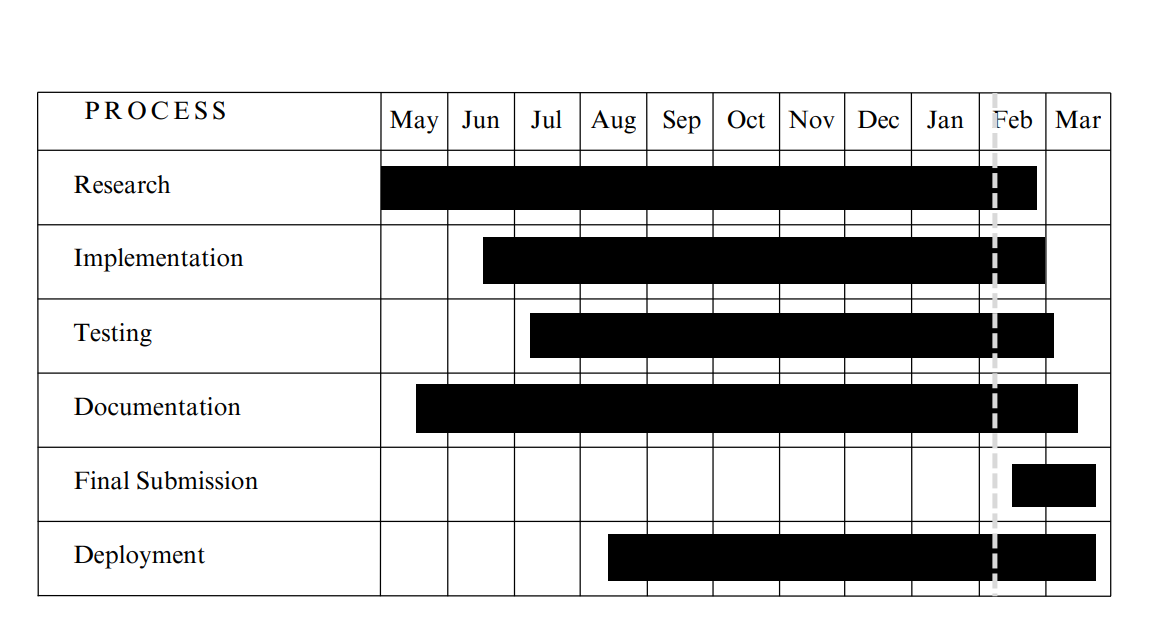
\includegraphics[width=\textwidth]{src/images/figures/gantt.png}
\end{table}


% \chapter{PLAGARISM SUMMARY}
% Keep all the pages of the plagarism summary document provided by the university here. It can run for multiple pages.

% \input{src/backmatter/studentGuide.tex}


% =====================
% REFERENCES
% =====================
\renewcommand{\bibname}{REFERENCES}
\bibliographystyle{IEEEtran}
\bibliography{references}

\end{document}
